\documentclass[12pt,a4paper,oneside]{report}

% Page layout
\usepackage[a4paper,top=1.7cm,bottom=7.4cm,left=2.5cm,right=6.0cm,footskip=6.3cm]{geometry}
\usepackage{setspace}
\usepackage{titlesec}
\usepackage{titling}
\usepackage{times}
\usepackage{fontspec}
\usepackage{algorithm}
\usepackage[noend]{algpseudocode}
\usepackage{pdflscape}  % For landscape pages
\usepackage{afterpage}  % For better page control

\setmainfont{Arial}
\usepackage{fancyhdr}
\pagestyle{fancy}
\fancyhf{}
\fancyfoot[C]{\thepage}
\renewcommand{\headrulewidth}{0pt}
\renewcommand{\footrulewidth}{0pt}

% Include PDF
\usepackage{pdfpages}
% Bibliography - numbered citations with square brackets using natbib
\usepackage[numbers,square,sort&compress]{natbib}

% Define MDPI-style commands
\newcommand{\authorcontributions}[1]{\section*{Author Contributions}#1}
\newcommand{\funding}[1]{\section*{Funding}#1}
\newcommand{\conflictsofinterest}[1]{\section*{Conflicts of Interest}#1}
\newcommand{\acknowledgments}[1]{\section*{Acknowledgments}#1}

\usepackage{url}
\usepackage{hyperref}
% math
\usepackage{amsmath}
% microtype for letter spacing and typography improvements
\usepackage{microtype}

% for Plant Count section
\usepackage{tabularx}         % For tabularx environment
\usepackage{float}            % For H float option
\usepackage{subfig}           % For subfloat command
\usepackage{changepage}       % For adjustwidth environment
\usepackage{booktabs}         % For toprule, midrule, bottomrule commands
\usepackage{cleveref}         % For \cref command


% Paragraph formatting
\setlength{\parskip}{6pt}
\setlength{\parindent}{0pt}
\setstretch{1.5}

% Define extralength parameter
\newlength{\extralength}
\setlength{\extralength}{0cm}

% Set section numbering to start from 2.1
\renewcommand\thesection{2.1.\arabic{section}}

\begin{document}

\abstract{Effective object detection in precision agriculture requires understanding 
minimum dataset requirements, yet this remains undetermined for arable crops seedling detection. 
This study investigates the minimum dataset size and quality needed to achieve benchmark 
performance (R² = 0.85) across different object detection paradigms. We systematically 
evaluated many-shot models (YOLOv5, YOLOv8, YOLO11, RT-DETR), few-shot (CD-ViTO), 
and zero-shot (OWLv2) approaches using orthomosaic imagery of maize seedlings, while 
also implementing a handcrafted algorithm as baseline. Models were tested with varying 
dataset sizes, quality levels, and training sources (in-domain vs out-of-distribution). 
Results demonstrate that no out-of-distribution trained model achieved benchmark 
performance, while in-domain trained models reached the benchmark with 60-130 annotated 
images, depending on architecture. Transformer-mixed models (RT-DETR) required fewer 
samples (60) than CNN-based models (110-130), but showed different sensitivities 
to annotation quality reduction. Models maintained benchmark performance with 65-90\% 
of original annotation quality. Neither few-shot nor zero-shot approaches met benchmark 
requirements despite their recent advances. These findings provide practical guidance 
for efficiently developing maize seedling detection systems, emphasizing that successful 
deployment requires in-domain training data, with minimum requirements dependent 
on model architecture.}

\clearpage
\setcounter{page}{65}
\thispagestyle{fancy}
\section{Introduction} 

\subsection{Arable Crop Plant Counting by Object Detection}

Plant counting is a critical operation in precision agriculture, plant breeding, 
and agronomical evaluation. 
Accurate plant detection and counting in agricultural applications serves multiple critical functions:

\begin{enumerate}
    \item Crop Establishment Assessment: Early-season seedling counts determine whether or not replanting is necessary, 
    directly affecting yield potential and economic returns~\cite{blandinoeffetto2016}.
    \item Precision Agriculture: Individual plant locations enable variable-rate application of inputs (fertilizers, 
    pesticides) and selective harvesting, reducing costs and environmental impact~\cite{10287390}.
    \item Plant Breeding Programs: Automated counting accelerates phenotyping workflows, enabling evaluation of 
    larger populations and more traits~\cite{Saatkamp2019AResearchAF}.
    \item Insurance and Compliance: Standardized counting methods support crop insurance assessments and regulatory 
    compliance for agricultural subsidies~\cite{rs13051030}.
    \item Research Applications: Consistent counting methods enable meta-analyses across studies and reproducible
    research in agronomy~\cite{PP13332024}.
\end{enumerate}

Traditionally performed manually, this labor-intensive
task is increasingly automated through computer vision~algorithms.

To validate any counting method, establishing a performance benchmark is essential.
Such benchmarks can derive from manual counting accuracy, international standards,
or comparison with established methods. According to the European Plant Protection
Organization, acceptable plant counting methods must achieve a coefficient of 
determination (R²) of 0.85 when compared to manual counting~\cite{PP13332024}, 
corresponding to a Root Mean Square Error (RMSE) of approximately 0.39. This same
benchmark (R² = 0.85) is widely recognized in the scientific literature~\cite{zouMaizeTasselsDetection2020}.

In agricultural applications specifically, object detection offers advantages over
regression-based counting methods. Studies show object detection not only achieves
superior accuracy~\cite{zouMaizeTasselsDetection2020} but also provides geographical
plant coordinates when applied to georeferenced orthomosaics, rather than just density
estimates. 
The validation of this ability relies on metrics such as Intersection over Union ({$IoU$}),
Average Precision ({$AP$}), and~Average Recall~\cite{linMicrosoftCOCOCommon2015} rather than on
the coefficient of~determination. 

Georeferenced orthomosaics—created through aerial photogrammetry from overlapping
images with Ground Control Points (GCPs) \cite{krausPhotogrammetryGeometryImages2011}—are 
particularly valuable for agricultural counting applications. Their fixed scale and
orientation to geographical coordinates simplify object detection by providing
consistent object sizes and eliminating perspective distortion.
However, georeferenced orthomosaics also present certain limitations. Georeferencing 
errors due to low-quality or insufficient GCPs, or~reliance on onboard GNSS/IMU 
systems, can significantly reduce spatial accuracy.
This is particularly the case in datasets derived from unmanned aerial vehicles~\cite{pugh_comparison_2021,dhonju_web_2023}. Moreover, 
distortions may persist in areas with high relief or vegetation canopy variability 
if digital elevation models are inadequately detailed~\cite{habib_automated_2016,de_petris_rpas-based_2020}. 
Finally, computational demand and processing time during photogrammetric reconstruction 
remain a constraint, particularly for high-resolution or large-area orthomosaics~\cite{zhang_georeferencing_2022}.

Like many computer vision tasks in specialized domains, agricultural plant counting
suffers from data scarcity~\cite{farjon_deep-learning-based_2023}. 
Public datasets are limited and often lack critical 
information like orthorectification parameters or precise scale information. To~focus
our investigation, we selected grain maize seedlings ({\em Zea mays} L.) at the V3--V5 
growth stage~\cite{meierBBCHSystemCoding2009} as our case study, as~this crop is well
represented in both the scientific literature~\cite{davidPlantDetectionCounting2021,
liuIntegrateNetDeepLearning2022} and public repositories~\cite{Maize_seedingDatasetOverview,
MaizeseedlingdetectionDatasetOverview}.

Maize, the world's highest-production crop~\cite{fao2024}, offers ideal characteristics
for object detection at this growth stage. Its regular planting pattern with defined
inter-row and intra-row spacing, minimal overlapping, and~distinctive appearance makes
it suitable for automated counting. These characteristics are shared by other row crops
like sunflower ({\em Helianthus annuus} L.) and sugarbeet ({\em Beta vulgaris} L.), potentially
making our findings applicable to a broader range of agricultural scenarios~\cite{torres-sanchez_early_2021}.

\subsection{Evolution of Object Detection Methods}

The broader field of object detection has evolved from non-machine learning methods,
here named Handcrafted (HC) methods, 
to sophisticated Deep Learning (DL) approaches. Handcrafted methods rely on 
explicitly programmed rules and traditional computer vision techniques such as 
color thresholding, edge detection, and~morphological operations to identify 
objects. These approaches require domain expertise to design feature extraction 
algorithms but offer interpretability and computational efficiency~\cite{zhang2020cut,davidPlantDetectionCounting2021}. 
While state-of-the-art 
detection now relies primarily on DL, HC methods still find application in 
agricultural contexts~\cite{davidPlantDetectionCounting2021,garcia-martinezDigitalCountCorn2020}.

Modern DL object detection architectures fall into two main categories: those based
on Convolutional Neural Networks (CNNs) \cite{lecunDeepLearning2015} like Faster R-CNN
~\cite{FasterRCNNRealTime} and YOLO~\cite{YouOnlyLook}, and~those employing Transformer
architectures~\cite{vaswaniAttentionAllYou2017} like DETR~\cite{carionEndtoEndObjectDetection2020}, or hybrid approaches combining both paradigms. The~fundamental difference lies in how
images are processed—CNNs use grid-based convolutions while Transformers process
image patches using attention mechanisms~\cite{dosovitskiyImageWorth16x162021}.

On standard computer vision benchmarks like COCO~\cite{linMicrosoftCOCOCommon2015} 
and ImageNet~\cite{14090575ImageNetLarge}, Transformer-based approaches generally
outperform CNN-based models in accuracy~\cite{zongDETRsCollaborativeHybrid2023}. 
However, in~agricultural applications specifically, CNN-based architectures like YOLO
variants remain widely used due to their efficiency with smaller images and lower
computational requirements~\cite{khanSurveyVisionTransformers2023, 
badgujarAgriculturalObjectDetection2024}. For~agricultural deployment with limited
training data, Transformer-based models may offer advantages in fine-tuning scenarios
~\cite{rekavandiTransformersSmallObject2023,liTransformerObjectDetection2023}.

For our comparative analysis of agricultural object detection approaches, we selected
representative architectures from both paradigms. From~the CNN family, we chose YOLOv5
and YOLOv8 due to their widespread agricultural adoption~\cite{badgujarAgriculturalObjectDetection2024}.
From Transformer-mixed architectures, we selected RT-DETR~\cite{zhaoDETRsBeatYOLOs2024}
and YOLO11~\cite{khanamYOLOv11OverviewKey2024}, which demonstrate state-of-the-art
performance on standard~benchmarks.

\subsection{Data-Efficient Detection~Methods}

A critical challenge in agricultural object detection is the high cost of data 
annotation. Recently, emerging paradigms like zero-shot and few-shot object detection
offer potential solutions by reducing or eliminating annotation requirements. These
approaches differ fundamentally from traditional ``many-shot'' detectors in their data
needs.

In few-shot detection, models learn to identify objects from minimal examples—often
just 1--30 annotated instances (or ``shots''). These methods typically leverage feature
transfer or meta-learning~\cite{liMetaSGDLearningLearn2017} to generalize from 
limited data. The~agricultural potential of such approaches is significant, as~they
could drastically reduce annotation burden for new crop varieties or growth~stages.

Zero-shot detection represents the extreme case where models detect novel objects
without any labeled examples by exploiting semantic relationships or contextual
information learned from other classes~\cite{bansalZeroShotObjectDetection2018}.
State-of-the-art zero-shot detectors include YOLO-World~\cite{kangFewshotObjectDetection2019},
OWLv2~\cite{mindererScalingOpenVocabularyObject2023}, and~Grounding DINO
~\cite{liuGroundingDINOMarrying2025}.

While these data-efficient approaches show promise in general computer vision tasks,
their effectiveness for agricultural applications remains largely unexplored. For~maize seedling detection specifically, only two studies have investigated few-shot
methods~\cite{karamiAutomaticPlantCounting2020,wangAdvancingImageRecognition2024},
with neither achieving benchmark performance or clearly specifying shot counts. No
studies have yet evaluated zero-shot detection for maize seedling~counting.

\subsection{Dataset Requirements for Agricultural Object~Detection}

While general object detection benchmarks provide standardized evaluation, they poorly
represent agricultural conditions. Numerous studies have addressed plant detection in
field settings~\cite{barretoAutomaticUAVbasedCounting2021,liuIntegrateNetDeepLearning2022,
kitanoCornPlantCounting2019}, but~few have systematically investigated minimum dataset
requirements for robust performance~\cite{davidPlantDetectionCounting2021,
andvaagCountingCanolaGeneralizable2024}.

This knowledge gap creates significant challenges for practitioners who must determine
how much data to collect and annotate for effective deployment. The~agricultural
domain's unique characteristics—variable environment, specific plant phenotypes, and~orthomosaic imagery—may substantially alter data requirements compared to general
computer vision~tasks.

General deep learning principles suggest model performance correlates strongly with
training data quantity~\cite{sunRevisitingUnreasonableEffectiveness2017} and quality
~\cite{alhazmiEffectsAnnotationQuality2021}. These relationships can be modeled using
empirical approaches~\cite{hestnessDeepLearningScaling2017,mahmoodHowMuchMore2022}.
Other factors affecting minimum dataset requirements include model architecture
~\cite{nguyenEvaluationDeepLearning2020}, backbone selection~\cite{duSpineNetLearningScalePermuted2020},
and data augmentation strategies~\cite{shortenSurveyImageData2019}.

The most critical factor, however, appears to be dataset source. Studies consistently
show that using in-domain data (from the same distribution as the inference target)
dramatically improves accuracy while reducing required dataset size compared to
out-of-distribution training~\cite{davidPlantDetectionCounting2021,
andvaagCountingCanolaGeneralizable2024}. This finding has profound implications for
agricultural deployment~scenarios.

\subsection{Study~Aim}

This study aims to establish the minimum dataset requirements for accurate maize
seedling detection in georeferenced orthomosaics across different object detection
paradigms. Here, the~dataset size and quality are respectively defined as the amount of
annotated images in the training set and~the accuracy of the annotations.
In particular, the~annotation quality is defined as the percentage of correct
annotations relative to the total ground truth annotations present in each image, 
with 100\% representing perfect annotations where every plant is correctly identified 
and bounded. For~example, if~an image contains 10 plants and the annotator correctly 
identifies and bounds 8 of them, the~annotation quality for that image would be 80\%. 
To simulate varying annotation quality levels, we systematically removed a percentage 
of existing annotations from our complete ground truth dataset, effectively simulating 
scenarios where human annotators miss a certain proportion of plants due to factors 
such as time constraints, fatigue, or~challenging visual conditions. This approach 
allows us to evaluate how robust different models are to incomplete annotations, 
which is a common real-world scenario in agricultural applications where exhaustive 
annotation can be prohibitively expensive or time-consuming.
Specifically, we investigate the following:

\begin{enumerate}
    \item How training data source (in-domain vs. out-of-distribution) affects required dataset~size
    \item Minimum dataset size needed to achieve benchmark performance (R² = 0.85) for different model architectures
    \item Minimum annotation quality required to maintain benchmark performance
    \item Whether or not newer few-shot and zero-shot approaches can meet agricultural performance standards with reduced annotation requirements
    \item The potential role of handcrafted methods in modern deep learning pipelines
\end{enumerate}

By systematically varying training dataset size (10--150 images), annotation quality
(10--100\%), and~evaluating diverse architectures (CNN-based, Transformer-based,
few-shot, and~zero-shot), we provide comprehensive guidance for implementing efficient
maize seedling detection systems. Our findings establish empirical relationships
between dataset characteristics and model performance, offering practical insights
for optimizing the annotation effort versus detection performance trade-off in
agricultural object~detection.

%%%%%%%%%%%%%%%%%%%%%%%%%%%%%%%%%%%%%%%%%%
\section{Materials and~Methods}
\unskip

\subsection{Datasets}
The datasets used in this study to train the object detection models for maize seedling
counting are nadiral or supposedly nadiral images of maize seedlings at the V3--V5 growth stage,
or estimated so.
The V3--V5 growth stage is defined by the BBCH scale as the stage where the third to fifth
leaf is unfolded and the plant is 15--30 cm tall~\cite{meierBBCHSystemCoding2009}.

\textls[-15]{This study uses two dataset sources as training sets: the Out-of-Distribution  (OOD) dataset
and the In-Domain (ID) dataset. The ID datasets are from the same source as the
testing dataset, while the OOD datasets are not.
The OOD datasets are composed of images from scientific literature~\cite{liuEstimatingMaizeSeedling2022,davidPlantDetectionCounting2021}
and from internet repositories~\cite{Maize_seedingDatasetOverview,MaizeseedlingdetectionDatasetOverview}.
The ID datasets were collected during this study. This ID dataset creation consisted of
capturing nadiral images of three study areas with a Phantom 4 Pro v2.0 (DJI, Shenzhen, China)
drone equipped with its default series RGB camera at about 10 m above ground for 
a Ground Sampling Distance (GSD) of 2.7 mm/pixel.
The number of images captured depends on the study area size, which was about 2 hectares
for the ID\_1 location and about 1 ha for the other two.
For each location, an~orthomosaic was created using photogrammetric software.
Bundle adjustment error was estimated as 38 mm using the GCPs
surveyed by GNSS operating in VRS-NRTK mode. The~orthomosaics were generated with an 
average GSD of 5 mm/pixel in the WGS84/UTM 32 N reference system. We chose this 
GSD because it is the minimum GSD that allows the detection of maize seedlings at the V3--V5 growth stage
with a nadiral camera~\cite{velumaniEstimatesMaizePlant2021}.}

The OOD scientific datasets consist of tiles of georeferenced orthomosaics of maize seedlings from the scientific literature.
The OOD internet datasets consist of RGB images of maize seedlings from internet repositories.
The ID datasets were collected during this study and consist of tiles of georeferenced orthomosaics of maize seedlings of known scale.
The OOD scientific datasets and the ID datasets are composed of tiles of georeferenced orthomosaics 
of known scale, while the OOD internet datasets are simple RGB images of unknown scale.
All the OOD datasets came with annotations, while the ID datasets were manually annotated.
The OOD dataset annotations are rectangular bounding boxes centering on an individual plant stem.
ID dataset annotation was done during this study by an agronomist by observing the 
entire orthomosaic in a Geographical Information System (GIS) environment, 
with the tile grid
overlapping the orthomosaic to focus on target tiles without losing the surrounding
context, so without losing bordering plants. Annotations were created as squared 
bounding boxes of a size length equal to the minimum distance between two plants in the row, 
with each box centered on an individual seedling~stem. 

Table~\ref{tab:datasets} summarizes the datasets used in this study.

\begin{table}[H]
\caption{Summary of datasets used in the study.}
\label{tab:datasets}
\begin{tabularx}{\textwidth}{llXX}
\toprule
\textbf{Dataset} & \textbf{Phenological Stage} & \textbf{Train Size} & \textbf{Test Size} \\
\midrule
\multicolumn{4}{l}{OOD Scientific} \\
\hspace{0.5em}DavidEtAl.2021~\cite{davidPlantDetectionCounting2021} & V3 & 182 tiles & N/A* \\
\hspace{0.5em}LiuEtAl.2022~\cite{liuEstimatingMaizeSeedling2022} & V3 & 596 tiles & N/A* \\
\midrule
\multicolumn{4}{l}{OOD Internet} \\
\hspace{0.5em}OOD\_int\_1~\cite{Maize_seedingDatasetOverview} & V3 & 216 tiles & N/A* \\
\hspace{0.5em}OOD\_int\_2~\cite{MaizeseedlingdetectionDatasetOverview} & V5 & 174 tiles & N/A* \\
\midrule
\multicolumn{4}{l}{ID~\cite{bumbaca202515235602}} \\
\hspace{0.5em}ID\_1 & V3 & 150 tiles & 20 tiles \\
\hspace{0.5em}ID\_2 & V3 & 150 tiles & 20 tiles \\
\hspace{0.5em}ID\_3 & V5 & 150 tiles & 20 tiles \\
\bottomrule
\end{tabularx}
\noindent\footnotesize{* N/A indicates that these datasets were used only for training purposes and do not have separate test sets in this study.}
\end{table}
\vspace{-6pt}


To make the two types of datasets comparable, we chose to rescale the images to a scale of 0.005 m/pixel
where the scale was known (scientific OOD and ID datasets), obtaining orthomosaics of different sizes.
All the orthomosaics were then cropped to \mbox{224 $\times$ 224 pixel} tiles.
This tile size was selected because at 5 mm/pixel resolution it covers 1.12 × 1.12 m of field area.
Given that typical grain maize inter-row distance is 0.75 m, this size enables capturing 
approximately two rows per tile, which is optimal for row pattern identification in the HC algorithm 
and provides sufficient context for object detection models~\cite{davidPlantDetectionCounting2021,liuEstimatingMaizeSeedling2022}.
This particular image size was also chosen as a standard from AlexNet~\cite{krizhevskyImageNetClassificationDeep2012}
as it should be compatible with most of the object detection architectures.
The annotations were rescaled and cropped where needed.
Figure~\ref{fig:datasets} shows a sample for each dataset.
Each ID dataset has 20 tiles to be used as the testing dataset, while the other 
150 tiles are used as the training~dataset.

\begin{landscape}
\begin{figure}
  \centering
  \begin{adjustwidth}{-\extralength}{0cm}
  \subfloat[\centering]{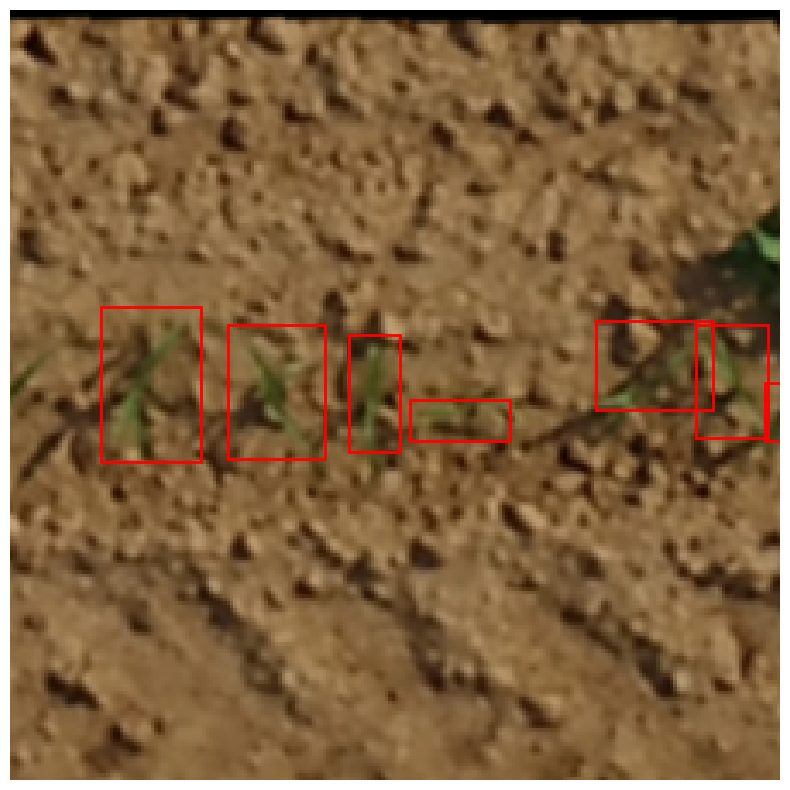
\includegraphics[width=4.5cm]{Plots/DavidEtAl.png}}
  \subfloat[\centering]{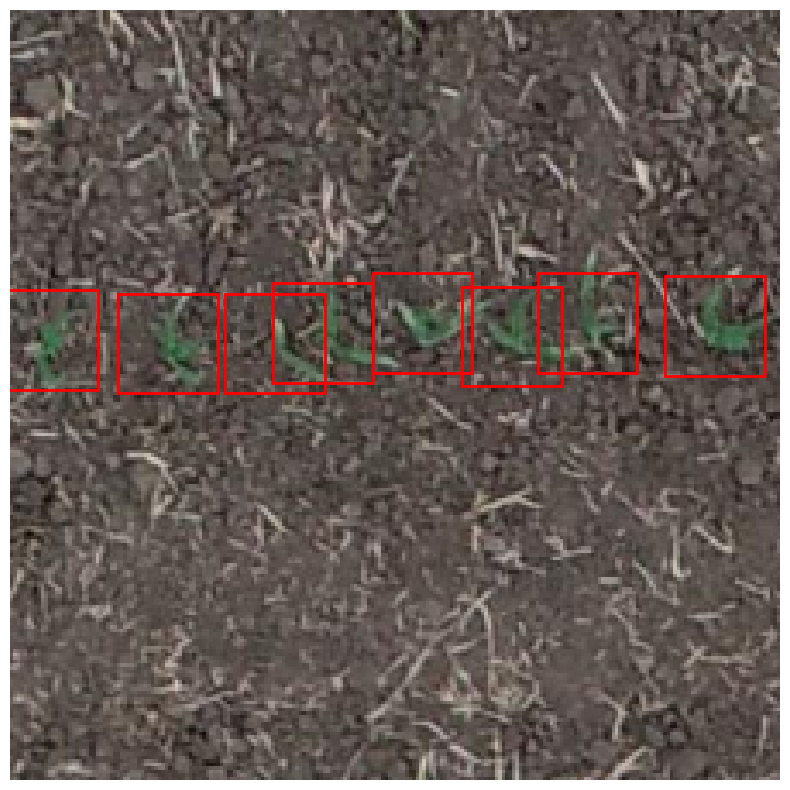
\includegraphics[width=4.5cm]{Plots/LiuEtAl.png}}
  \subfloat[\centering]{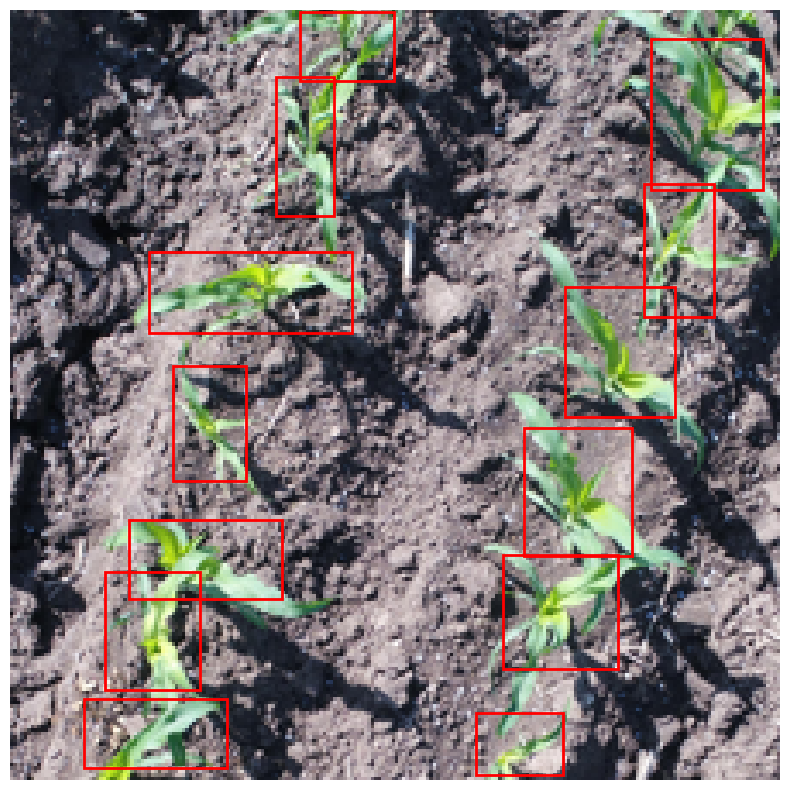
\includegraphics[width=4.5cm]{Plots/maize_seedling.png}}
  \subfloat[\centering]{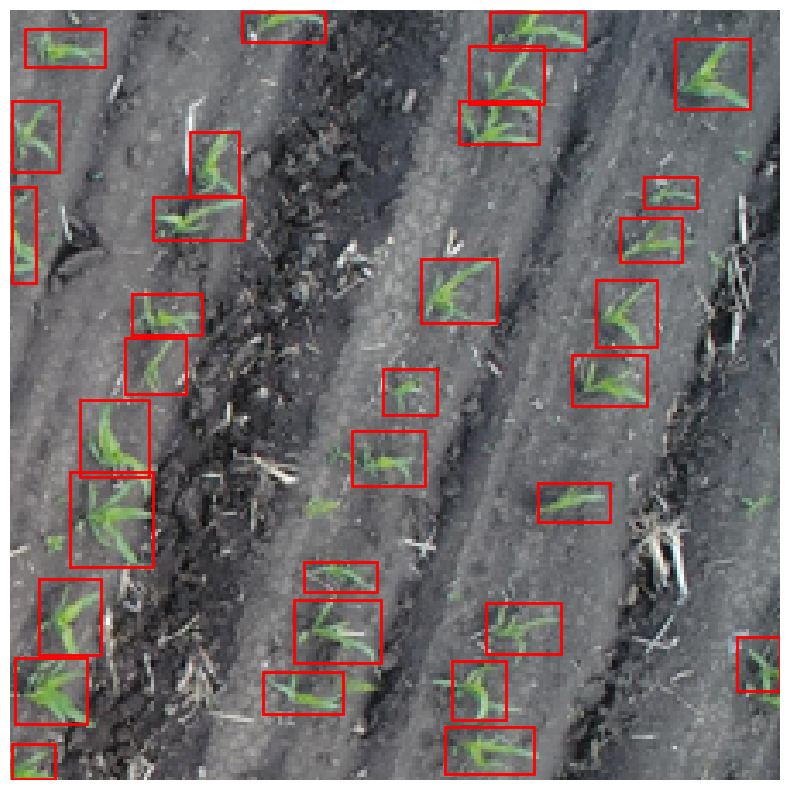
\includegraphics[width=4.5cm]{Plots/maize_seedling_detection.png}}\\
  \subfloat[\centering]{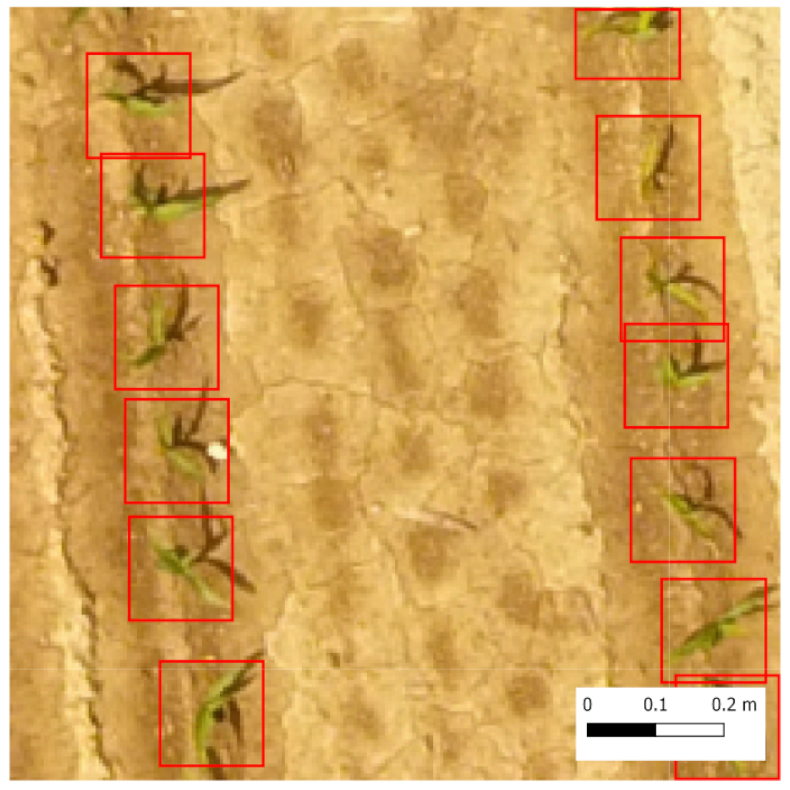
\includegraphics[width=6cm]{Plots/ID_1.png}}
  \subfloat[\centering]{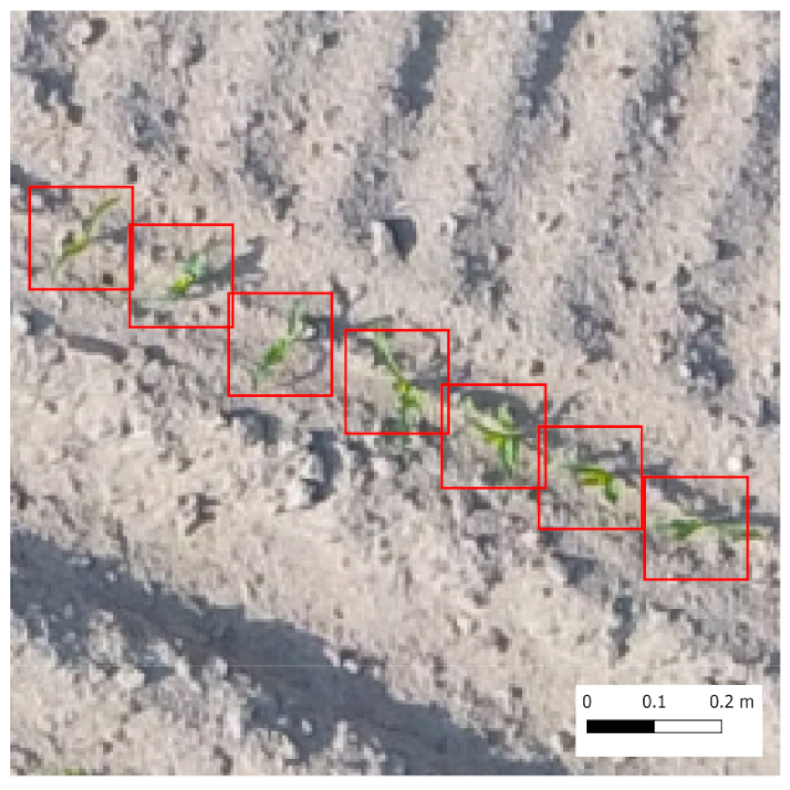
\includegraphics[width=6cm]{Plots/ID_2.png}}
  \subfloat[\centering]{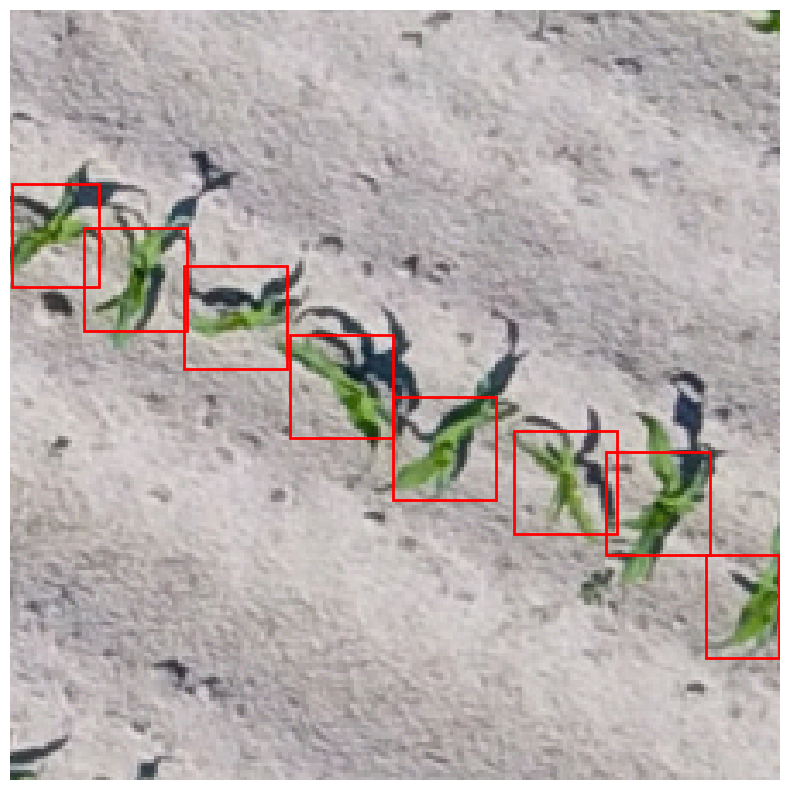
\includegraphics[width=6cm]{Plots/ID_3.png}}

\end{adjustwidth}
  \caption{Image examples taken from each dataset, ground truth bounding boxes are shown  in red. %MDPI: please confirm whether red frame in this figure need explanation. %Authors: Red frame shows bounding box annotations, explanation added
  (\textbf{a})~DavidEtAl.2021, 
 (\textbf{b}) LiuEtAl.2022, 
  (\textbf{c}) Internet Maize stage V3,
  (\textbf{d}) Internet Maize stage V5,
  (\textbf{e})~ID\_1,
  (\textbf{f})~ID\_2,
  (\textbf{g})~ID\_3.}
  \label{fig:datasets}  
\end{figure}
\end{landscape}

\subsection{Handcrafted Object~Detector}

Like other works~\cite{davidPlantDetectionCounting2021,garcia-martinezDigitalCountCorn2020,liuEstimatingMaizeSeedling2022},
we wrote an HC algorithm to obtain annotated tiles from the orthomosaics, 
basing it on agronomical knowledge and color thresholding.
Hue, Saturation, and Value (HSV) color space was used here to threshold the image,
to obtain green pixels, but~other color spaces can be used.
For the execution of this algorithm, the~following graphical and agronomical 
parameters must be set: color minimum and maximum thresholds (color threshold), the~minimum and maximum 
leaf area for the plant (leaf area range), the~minimum distance between plants on rows (intra-row distance),
and the distance between rows (inter-rows distance). 
The algorithm is expected to work on the orthomosaics of maize seedlings at the V3--V5 growth stage,
with low weed infestation, with~rows having roughly the same angle with meridian and distance between them.
The algorithm was implemented in Python 3.13.1 using the following packages: 
numpy (v 1.24.3), torch (\mbox{v 2.0.1}), PyYAML (v 6.0), rasterio (v 1.3.8), shapely (\mbox{v 2.0.1}), 
fiona (\mbox{v 1.9.4}), scikit-image (\mbox{v 0.21.0}), scikit-learn (v 1.3.0), matplotlib (v 3.7.1). 
The complete implementation is accessible from %MDPI: Please provide the date you accessed the URL in the following format: “URL (accessed on Day Month Year)”.
\url{https://gist.github.com/SamueleBumbaca/4a227bbe7b78d6be3424899c16c60bb4} (accessed on 20 June 2025).

The algorithm is divided in two sequential parts that form a detection--verification pipeline. The~first part,
named HC1 \cref{alg:H1}, performs initial plant detection by thresholding pixels within the specified color range, 
identifying connected regions, and~filtering them based on expected leaf area. HC1 outputs region polygons
representing potential plants, but~typically includes many false positives due to its simple color-based approach.
To address this limitation, we implemented a second process named HC2 \mbox{\cref{alg:H2}} that applies agronomical 
knowledge of field structure. HC2 filters the HC1 output by verifying that detected plants form proper row 
patterns with expected intra-row and inter-row spacing. It uses RANSAC~\cite{fischlerRandomSampleConsensus1987} to identify the linear alignments of plants 
and validates that these alignments match expected field geometry (consistent row slope and spacing).
Only tiles where HC2 confirms the expected number and arrangement of plants are retained for the final dataset.
This two-stage approach enables the automated extraction of high-confidence annotations from the orthomosaics.
Complete algorithm pseudocodes are provided in the~Appendix A.

\subsection{Deep Learning Object~Detectors}

\textbf{Many-shot model selection criteria}: %MDPI: Please confirm if the bold formatting is necessary; if not, please remove it. The following highlights are the same. %Authors: Bold formatting maintained
From the extensive landscape of available object detection architectures, we 
applied the following selection criteria: (1) widespread adoption in agricultural 
computer vision applications \cite{badgujarAgriculturalObjectDetection2024}, 
(2) availability of multiple model sizes to investigate parameter count effects 
on dataset requirements, (3) representation of different architectural paradigms 
(CNN-based vs. Transformer-based), (4) consistent implementation framework for 
fair comparison, and~(5) proven performance on small object detection tasks 
relevant to seedling identification.
The many-shot object detectors used in this study include YOLOv5, YOLOv8, RT-DETR, 
and YOLO11. Each represents distinct architectural approaches to object detection:

\begin{itemize}
  \item \textbf{YOLOv5} %Authors: Bold formatting kept for consistency 
  with model descriptions uses a CSP (Cross Stage Partial) backbone with a PANet neck 
  for feature aggregation, achieving efficient detection through grid-based prediction 
  with multiple anchors per cell. It was selected as the baseline CNN architecture due to its 
  dominance in agricultural applications~\cite{badgujarAgriculturalObjectDetection2024} 
  and extensive use in crop monitoring studies~\cite{kitanoCornPlantCounting2019,
  barretoAutomaticUAVbasedCounting2021}. Its CSP backbone with PANet neck provides 
  a well-established reference point for minimum dataset requirements in 
  agricultural~contexts.
  
  \item \textbf{YOLOv8} %Authors: Bold formatting kept for consistency 
  with model descriptions improves upon YOLOv5 by adopting a more efficient C2f block 
  in its backbone, implementing an anchor-free detection head and~using a task-specific 
  decoupled head design for better accuracy--speed trade-offs. It represents the next-generation YOLO evolution with 
  anchor-free detection and improved C2f blocks. We included it to evaluate 
  whether or not architectural improvements could reduce dataset requirements compared 
  to YOLOv5, given its reported superior accuracy--efficiency trade-offs~\cite{tervenComprehensiveReviewYOLO2023}.
  
  \item \textbf{YOLO11} %Authors: Bold formatting kept for consistency 
  with model descriptions further refines the architecture with multi-scale deformable 
  attention, improving small object detection—a crucial feature for seedling 
  identification in varied field conditions. It was chosen as the most recent YOLO 
  variant including an attention mechanisms (transformer). This selection allows us to 
  assess whether or not state-of-the-art Transformer-mixed improvements affect minimum dataset 
  requirements for small object~detection.
  
  \item \textbf{RT-DETR} %Authors: Bold formatting kept for consistency 
  with model descriptions represents a hybrid approach combining CNN backbones with 
  Transformer decoders, utilizing deformable attention for adaptive feature sampling 
  and parallel prediction heads for real-time performance. Unlike pure CNN-based YOLO 
  variants, RT-DETR's Transformer components enable the modeling of global relationships 
  between objects. We selected 
  it over pure Transformer models (like DETR) due to its real-time capabilities 
  and proven performance on agricultural datasets~\cite{zhaoDETRsBeatYOLOs2024}. 
  Its inclusion allows direct comparison between CNN-only and hybrid approaches 
  for minimum dataset~requirements.
\end{itemize}

\textbf{Excluded alternatives and rationale:} %Authors: Bold formatting kept for consistency 
with model descriptions
We deliberately excluded several model families: Faster R-CNN and other two-stage 
detectors due to their computational overhead and limited agricultural adoption; 
pure Transformer models like DETR due to prohibitive training requirements for 
small datasets~\cite{carionEndtoEndObjectDetection2020} 

We used the Ultralytics implementation 
for all models as it is open-source~\cite{jocherGitHubUltralyticsYOLO2023} and 
enables consistent parameter tuning across~architectures.

All model training and inference were performed on a workstation equipped with an 
Intel(R) Xeon(R) CPU E5-2670 v3 @ 2.30 GHz, 64.0 GB RAM, and~an NVIDIA RTX A5000 
GPU with 24 GB VRAM. The~computational constraints influenced certain experimental 
design choices, such as batch size and precision~settings.

For all many-shot models we used the same hyperparameters and augmentations as the
library default, with~the following exceptions:

\begin{itemize}
  \item batch size: 16 (increased from default 8 to maximize GPU utilization while 
  maintaining stable gradients)
  \item maximum training epochs: 200 (extended from default 100 to ensure 
  convergence with small datasets)
  \item maximum training epochs without improvement: 15 (increased from default 10 
  for early stopping to allow longer plateau exploration)
  \item precision: mixed (to balance training speed and numerical accuracy)
\end{itemize}

The default augmentations from the Ultralytics library include random scaling 
($\pm$10\%), random translation ($\pm$10\%), random horizontal flip (probability 0.5), 
HSV color space augmentation (hue $\pm$0.015, saturation $\pm$0.7, value $\pm$0.4), 
and mosaic augmentation. These augmentations were selected to reflect potential 
variations in field conditions without introducing unrealistic~distortions.

For few-shot detection, we employed CD-ViTO, which differs fundamentally from 
many-shot approaches:

\begin{itemize}
  \item \textbf{CD-ViTO} %Authors: Bold formatting kept for consistency 
  with model descriptions uses cross-domain prototype matching, where a small set 
  of annotated examples (shots) serves as class prototypes. It leverages Vision 
  Transformer (ViT) backbones to extract feature representations and computes 
  similarity between query images and prototypes for object localization. This 
  architecture is specifically designed for scenarios with limited training data.
\end{itemize}

The size of this model is determined by the backbone used: ViT-S, ViT-B, or~ViT-L~\cite{oquabDINOv2LearningRobust2024}. We used the implementation provided by the 
authors~\cite{fuCrossDomainFewShotObject2024}. In~our study, a~'shot' corresponds 
to an image with a single annotated plant. We tested 1, 5, 10, 30, and~50 shots, 
randomly selected from the ID manually labeled~dataset.

For zero-shot detection, we selected OWLv2:

\begin{itemize}
  \item \textbf{OWLv2} %Authors: Bold formatting kept for consistency 
  with model descriptions represents a fundamentally different paradigm that requires 
  no labeled examples of the target class. It leverages large-scale pre-training on 
  image--text pairs to establish connections between visual features and natural 
  language descriptions. During~inference, it detects objects based solely on 
  text prompts, eliminating the need for class-specific training data entirely.
\end{itemize}

We chose OWLv2 as our zero-shot exemplar because it represents state-of-the-art 
performance in open-vocabulary detection~\cite{mindererScalingOpenVocabularyObject2023,
liuGroundingDINOMarrying2025}. For~testing, we used the implementation from the 
Transformers library~\cite{wolfTransformersStateoftheArtNatural2020} with 
the published parameters. We evaluated two encoder sizes (ViT-B/16, ViT-L/14) 
with three pre-training strategies:

\begin{itemize}
    \item \textbf{Base models}: %Authors: Bold formatting kept for consistency 
Trained using self-supervised learning with the 
    OWL-ST method, generating pseudo-box annotations from web-scale image--text 
    datasets.
    \item \textbf{Fine-tuned models}: %Authors: Bold formatting kept for consistency 
Further trained on human-annotated object 
    detection datasets.
    \item \textbf{Ensemble models}: %Authors: Bold formatting kept for consistency 
Combining multiple weight-trained versions to 
    balance open-vocabulary generalization and task-specific performance.
\end{itemize}

For all OWLv2 variants, we tested multiple text prompts to describe maize seedlings, 
ranging from simple terms (``maize'', ``seedling'') to more descriptive phrases 
(``aerial view of maize seedlings'', ``corn seedlings in rows''). The~complete list 
of eleven prompts is provided in the~Appendix A.

The choice of text prompt significantly influences OWLv2 performance, as~the model 
relies on semantic alignment between visual features and language descriptions 
learned during pre-training~\cite{zhu_harnessing_2024}. Simple generic terms like ``maize'' or ``plant'' may 
activate broader visual concepts that include mature plants or other crop types, 
potentially reducing detection specificity. Conversely, descriptive phrases like 
``aerial view of maize seedlings'' provide more contextual information that should 
theoretically improve alignment with our orthomosaic imagery~\cite{s24186109}. However, if~such 
specific descriptions were underrepresented in the pre-training data, they may 
perform worse than simpler terms~\cite{chen_taskclip_2024}. To~account for this variability, we evaluated 
all prompts systematically and report the results using the best-performing prompt 
for each model variant; Figure%MDPI:  The first citation of each figure should appears in numerical order, we detected that Figure 9 is before Figure 2, please check and revise!!!! %Authors: Figure order checked and revised
~9 shows 
the full distribution of performance across all tested~prompts.

\textls[-15]{\cref{tab:architectures} shows the architectures used in the study 
with their parameter size specifications.}

\begin{table}[H]
  \caption{Summary of tested architectures and model sizes.}
  \label{tab:architectures}
%  \centering
  \begin{tabularx}{\textwidth}{lXXXXXX}
  \toprule
  \textbf{Architecture} &\textbf{Shots} & \textbf{n * or S} & \textbf{s * or S} & \textbf{m * or B} & \textbf{l * or L} & \textbf{x *} \\
  \midrule
  YOLOv5 & many & 1.9 & 7.2 & 21.2 & 46.5 & 86.7 \\
  YOLOv8 & many & 3.2 & 11.2 & 25.9 & 43.7 & 68.2 \\
  YOLO11 & many & 4.0 & 12.5 & 28.0 & 50.0 & 75.0 \\
  RT-DETR & many & - & - & - & 60.0 & 80.0 \\
  CD-VITO & few & - & 22.0 † & 86.0 ‡ & 307.0 § & - \\
  OWLv2 & zero & - & - & 86.0 ‡ & 307.0 § & - \\
  \bottomrule
  \end{tabularx}
\noindent{\footnotesize{ %MDPI: there is no * in this table, please confirm whether this explanation should be removed!!!! %Authors: Asterisk removed
 Values %MDPI: We merged the table footer into one paragraph. Please confirm. %Authors: Confirmed
 represent millions of~parameters. * Model size variants stand for nano (n), small (s), medium (m), large~(l), and~extra-large (x). † ViT-S (Small) backbone. ‡ ViT-B (Base) backbone. § ViT-L (Large) backbone.}}
\end{table}
\unskip

\subsection{Minimum Dataset Size and Quality~Modelling}
In order to investigate the minimum size and quality of the dataset required to train 
a robust object detection model for maize seedling counting, we conducted a series of experiments
where the above mentioned DL models were recursivelly fitted with increasing dataset size and quality.
To evaluate the HC object detector on the ID dataset,
we measured three key aspects: (1) the number of tiles that the HC algorithm 
successfully annotated from the orthomosaics (tiles%MDPI: Please confirm if the italics are necessary; if not, please remove them. The following highlights are the same. %Authors: Italics formatting checked and unified
), (2) this number as a percentage 
of the total available dataset (dataset\%), and~(3) the detection accuracy compared to 
manual annotations using standard metrics ($R^2$, $RMSE$, $MAPE$%MDPI: The format of equation variables (italics, bold, superscript, uppercase, lowercase, etc.) should be consistent throughout the paper (main text, tables, figures, equations). Please double check all the cases in the paper and unify them carefully. The following highlights are the same. %Authors: Variable formatting checked and unified throughout
, and~$mAP$).
For many-shot models we consider a training 
dataset split of 10\% validation and 90\% training, while for few-shot the number of shots
determined the amount of training samples. Zero-shot learning relies only on descriptions of the objects to be detected in natural language. Thus, the~effects of the prompts were evaluated.
As previously mentioned, this involved testing multiple text prompts.
For what concerns only the dataset size evaluation, for~many-shot models we considered
sizes from 10 to 150 images in 15 steps of 10 images, while for few-shot models we considered
1, 5, 10, 30, and~50 shots.
As concerns the dataset quality, we evaluated the annotation quality by reducing
the number of annotations per image from 100\% to 10\% in 10 steps of 10\% while
keeping the dataset size constant.
To evaluate the influence of dataset source (OOD or ID) on the model performance, we trained
the models using both OOD and ID datasets with the same experimental protocol.
Only the most relevant results are~reported.

For all the models, we evaluated the relationship between dataset size or quality and model performance
using $R^2$ and $mAP$, respectively, for plant counting and plant detection. Whether or not
$R^2$ provided values below $-$1~\cite{chicco_coefficient_2021}, we also considered 
$RMSE$ as the metric for counting~\cite{draper1998applied}.
$MAPE$ was considered for few-shot and zero-shot models only to evaluate the 
quality of the annotations produced by the prediction of these models.
We list here the metrics formulas for clarity:
\begin{align}
R^2 &= 1 - \frac{\sum_{i=1}^{n} (y_i - \hat{y}_i)^2}{\sum_{i=1}^{n} (y_i - \bar{y})^2}
\end{align}
where $y_i$ is the ground truth count for the $i$-th image, $\hat{y}_i$ is the 
predicted count, and~$\bar{y}$ is the mean of all ground truth counts. $R^2$ ranges 
from $-\infty$ to 1, with~1 indicating perfect prediction, 0 indicating that the 
model predictions are no better than simply predicting the mean, and~negative 
values indicating that the model performs worse than predicting the mean~\cite{chicco_coefficient_2021,draper1998applied}.
\begin{align}
\text{$RMSE$} &= \sqrt{\frac{1}{n}\sum_{i=1}^{n} (y_i - \hat{y}_i)^2}
\end{align}
where $RMSE$ measures the average magnitude of prediction errors in the original 
units (number of plants) for each image~\cite{draper1998applied}.
\begin{align}
\text{$MAPE$} &= \frac{100\%}{n}\sum_{i=1}^{n} \left| \frac{y_i - \hat{y}_i}{y_i} \right|
\end{align}
where $MAPE$ measures the percentage error relative to the actual values, providing a scale-independent 
measure of accuracy. It is expressed as a percentage, with~lower values indicating a lower
percentage of false positives or false negatives.
Thus, it was reported as an index of the quality of the annotations.
Note that $MAPE$ is only calculated for cases where $y_i \neq 0$ to avoid division by zero.
It is particular useful for counting as testing tiles never have zero plants~\cite{ARMSTRONG199269}.

For object detection performance, we used the standard COCO evaluation \mbox{metric~\cite{linMicrosoftCOCOCommon2015,everingham_pascal_2010}}:
\begin{align}
\text{$mAP$} &= \frac{1}{|IoU|}\sum_{t \in IoU}\text{AP}_t
\end{align}
where $mAP$ (mean Average Precision) is calculated at a single IoU %MDPI: The format of equation variables (italics, bold, superscript, uppercase, lowercase, etc.) should be consistent throughout the paper (main text, tables, figures, equations). Please double check all the cases in the paper and unify them carefully. The following highlights are the same. %Authors: Variable formatting checked and unified throughout
 (Intersection over Union) 
threshold of 0.5.
AP at the IoU threshold is the area under the precision--recall curve for detections 
that meet that IoU threshold~criterion.

To test the predictability minimum dataset size and quality required to train a robust
(achieving benchmark) object detector for maize seedling counting through empirical 
models, we test the logarithmic, arctan, and algebraic root functions to fit the 
dataset size or quality versus performance relationships, as suggested by previous
studies~\cite{mahmoodHowMuchMore2022}. 

These functions were selected because they represent different theoretical behaviors 
commonly observed in machine learning scaling studies:

\textbf{Logarithmic function:} %Authors: Bold formatting kept for consistency 
Models the diminishing returns pattern where initial 
data additions provide substantial performance gains, but~additional data yield progressively smaller improvements. This behavior is theoretically grounded in 
learning theory, where models approach their optimal performance asymptotically~\cite{hestnessDeepLearningScaling2017}.

\textbf{Arctangent function:} %Authors: Bold formatting kept for consistency 
Represents a saturating behavior where performance 
increases rapidly at first, then approaches a plateau. This function is particularly 
suitable for modeling performance metrics bounded by theoretical limits (e.g., R² 
approaching 1.0) and captures scenarios where models reach their maximum capacity 
given architectural constraints~\cite{vianna_analysis_2024}.

\textbf{Algebraic root function:} %Authors: Bold formatting kept for consistency 
Models power-law relationships between dataset 
size and performance, allowing for various growth rates depending on the exponent. 
This function can capture both sub-linear and super-linear scaling behaviors, 
providing flexibility for different model architectures and learning dynamics
~\cite{hestnessDeepLearningScaling2017}.

For clarity, we list here the functions tested:
\begin{align}
\text{Logarithmic: } f(x) &= a \ln(x) + b
\end{align}

\vspace{-24pt}

\begin{align}
\text{Arctan: } f(x) &= a \arctan(bx) + c
\end{align}

\vspace{-24pt}
\begin{align}
\text{Algebraic Root: } f(x) &= a x^{1/b} + c
\end{align}
where $x$ represents dataset size (number of images) or quality (percentage of 
correct annotations) and~$a$, $b$, and~$c$ are fitted parameters that determine 
the shape and scale of each~function.

For each model architecture and metric combination, we fitted all three functions 
to the observed dataset size versus performance data points using least squares 
regression. The~function yielding the highest goodness-of-fit was selected as the 
best predictor for that specific model--metric combination. This approach allows us 
to identify which scaling pattern best describes each model's behavior and enables 
prediction of the minimum dataset size required to achieve benchmark~performance.

The selected empirical model can then be used to interpolate or extrapolate 
performance estimates for untested dataset sizes, providing practical guidance 
for annotation planning. For~instance, if~a logarithmic function best fits the 
data, practitioners can expect diminishing returns from additional annotations 
beyond a certain point. Conversely, if~an algebraic root function provides the 
best fit, the~scaling behavior may indicate more linear or super-linear returns, 
suggesting different annotation~strategies.

For the model fits to dataset size versus performance relationships, we evaluated 
multiple fitting functions and selected the one with the highest goodness-of-fit:
\begin{align}
\text{$GoF$} &= R^2_{\text{fit}} = 1 - \frac{\sum_{i=1}^{n} (y_i - f(x_i))^2}{\sum_{i=1}^{n} (y_i - \bar{y})^2}
\end{align}
where $y_i$ is the observed metric (either $R^2$ or $mAP$), $f(x_i)$ is the 
fitted value at dataset size $x_i$, and~$\bar{y}$ is the mean of the observed 
metrics.

All the trained models were tested on the testing dataset tiles with the SAHI method~\cite{akyonSlicingAidedHyper2022}.
SAHI (Slicing Aided Hyper Inference) is a technique designed to improve object detection 
performance on high-resolution images by addressing the scale mismatch between training 
and inference conditions. The~method slices the testing image into smaller overlapping 
segments (patches) of the same size as the training tiles (224 × 224 pixels in our case) 
and then applies the model to each patch independently. The~model outputs from each 
patch are then merged using non-maximum suppression to eliminate duplicate detections, 
and the final results are cropped to the original tile~boundaries.

The use of SAHI is justified in our context because while models are trained on 
\mbox{224 × 224 pixel} tiles, the~real-world application involves inference on larger 
orthomosaics where objects may be partially occluded by tile boundaries or appear 
at different scales. SAHI overcomes this limitation by ensuring that all potential 
objects are evaluated by the model as complete entities rather than fragmented 
across tile boundaries. This approach is expected to provide better performance 
compared to using single tiles as input, as~it reduces boundary effects and 
maintains consistent object scale during~inference.

The predictions were then thresholded by a list of confidence score thresholds to obtain the plant count.
All the metrics were computed for different score thresholds for all the models
to evaluate the model performance at different confidence levels.
The values to thresholds bounding boxes score were 0, 0.05, 0.1, 0.15, 0.2, 0.25, 0.29, 0.4, 0.5, 0.6, 0.7, 0.8, 0.9, 0.95, 0.99.
The highest $R^2$ value within the thresholds was considered as the model 
performance for that experiment.
%%%%%%%%%%%%%%%%%%%%%%%%%%%%%%%%%%%%%%%%%%
\section{Results}
\unskip

\subsection{Handcrafted Object~Detector}

Table~\ref{tab:HC_results} shows the performance of the HC object detector on the ID datasets 
by enumerating metrics and successfully annotated tiles. The~metrics were computed
on the testing dataset~tiles.

\begin{table}[H]
  \caption{HC object detector~performance.}
  \label{tab:HC_results}
  \centering
  \begin{tabularx}{\textwidth}{lXXXXXX}
  \toprule
  \textbf{Dataset} & \boldmath{$R^2$} & \boldmath{$RMSE$} & \boldmath{$MAPE$} & \boldmath{$mAP$} & \textbf{Tiles} & \textbf{Dataset \%} \\
  \midrule
  ID\_1 & 0.95 & 0.12 & 9\% & 0.87 & 1184 & 7.8\% \\
  ID\_2 & 0.93 & 0.11 & 12\% & 0.81 & 279 &  4.2\% \\
  ID\_3 & 0.87 & 0.18 & 16\% & 0.73 & 158 & 1.8\% \\
  \bottomrule
  \end{tabularx}
  \end{table}

The HC algorithm was able to extract a discrete amount of annotated tiles from the orthomosaics,
with a percentage of the dataset ranging from 1.8\% to 7.8\%.
Overall, the HC object detector performed well on this set, with $R^2$ values
above 0.85 for all the datasets. The~$RMSE$ values were below 0.2, while the $mAP$ values
were above 0.7. The~MAPE values were below 20\% for all the~datasets.

In nominal scale, the number of tiles successfully annotated by the HC algorithm was
not constant, but~always over 150~tiles.

\subsection{Many-Shot Object~Detectors}

\subsubsection{OOD~Training}

The OOD scientific datasets ``DavidEtAl.2021'' and ``LiuEtAl.2022'' were tested singularly 
and in combination in the experiment named ``scientific OOD''. The~OOD internet datasets ``internet OOD''
were tested singularly and in combination with the OOD scientific datasets in the experiment named ``All OOD''.
Each model and OOD dataset combination was tested on the testing dataset tiles of the three ID~datasets.


None of the dataset combinations reached the benchmark $R^2$ value of 0.85 with any model.
The coefficients of determination and the root mean square errors 
for all the OOD experiments are shown in Figure~\ref{fig:metrics_OOD_datasets}.
The Goodness-of-Fit ($GoF$) values for the $R^2$ values were always low (below 0.2) for all the metrics.
The lowest $MAPE$ value was slightly less than 20\%. For~these same models, the $mAP$ values
were the highest, with~the best model being YOLOv8n with the LiuEtAl.2022 dataset.
No particular model size seems to provide better results with respect to the others, and
neither does the increasing dataset size seem to drive a model size performance trend.
As no model achieved the benchmark, no study was done on the dataset quality requirements
to achieve such~a benchmark.

\begin{landscape}
\begin{figure}
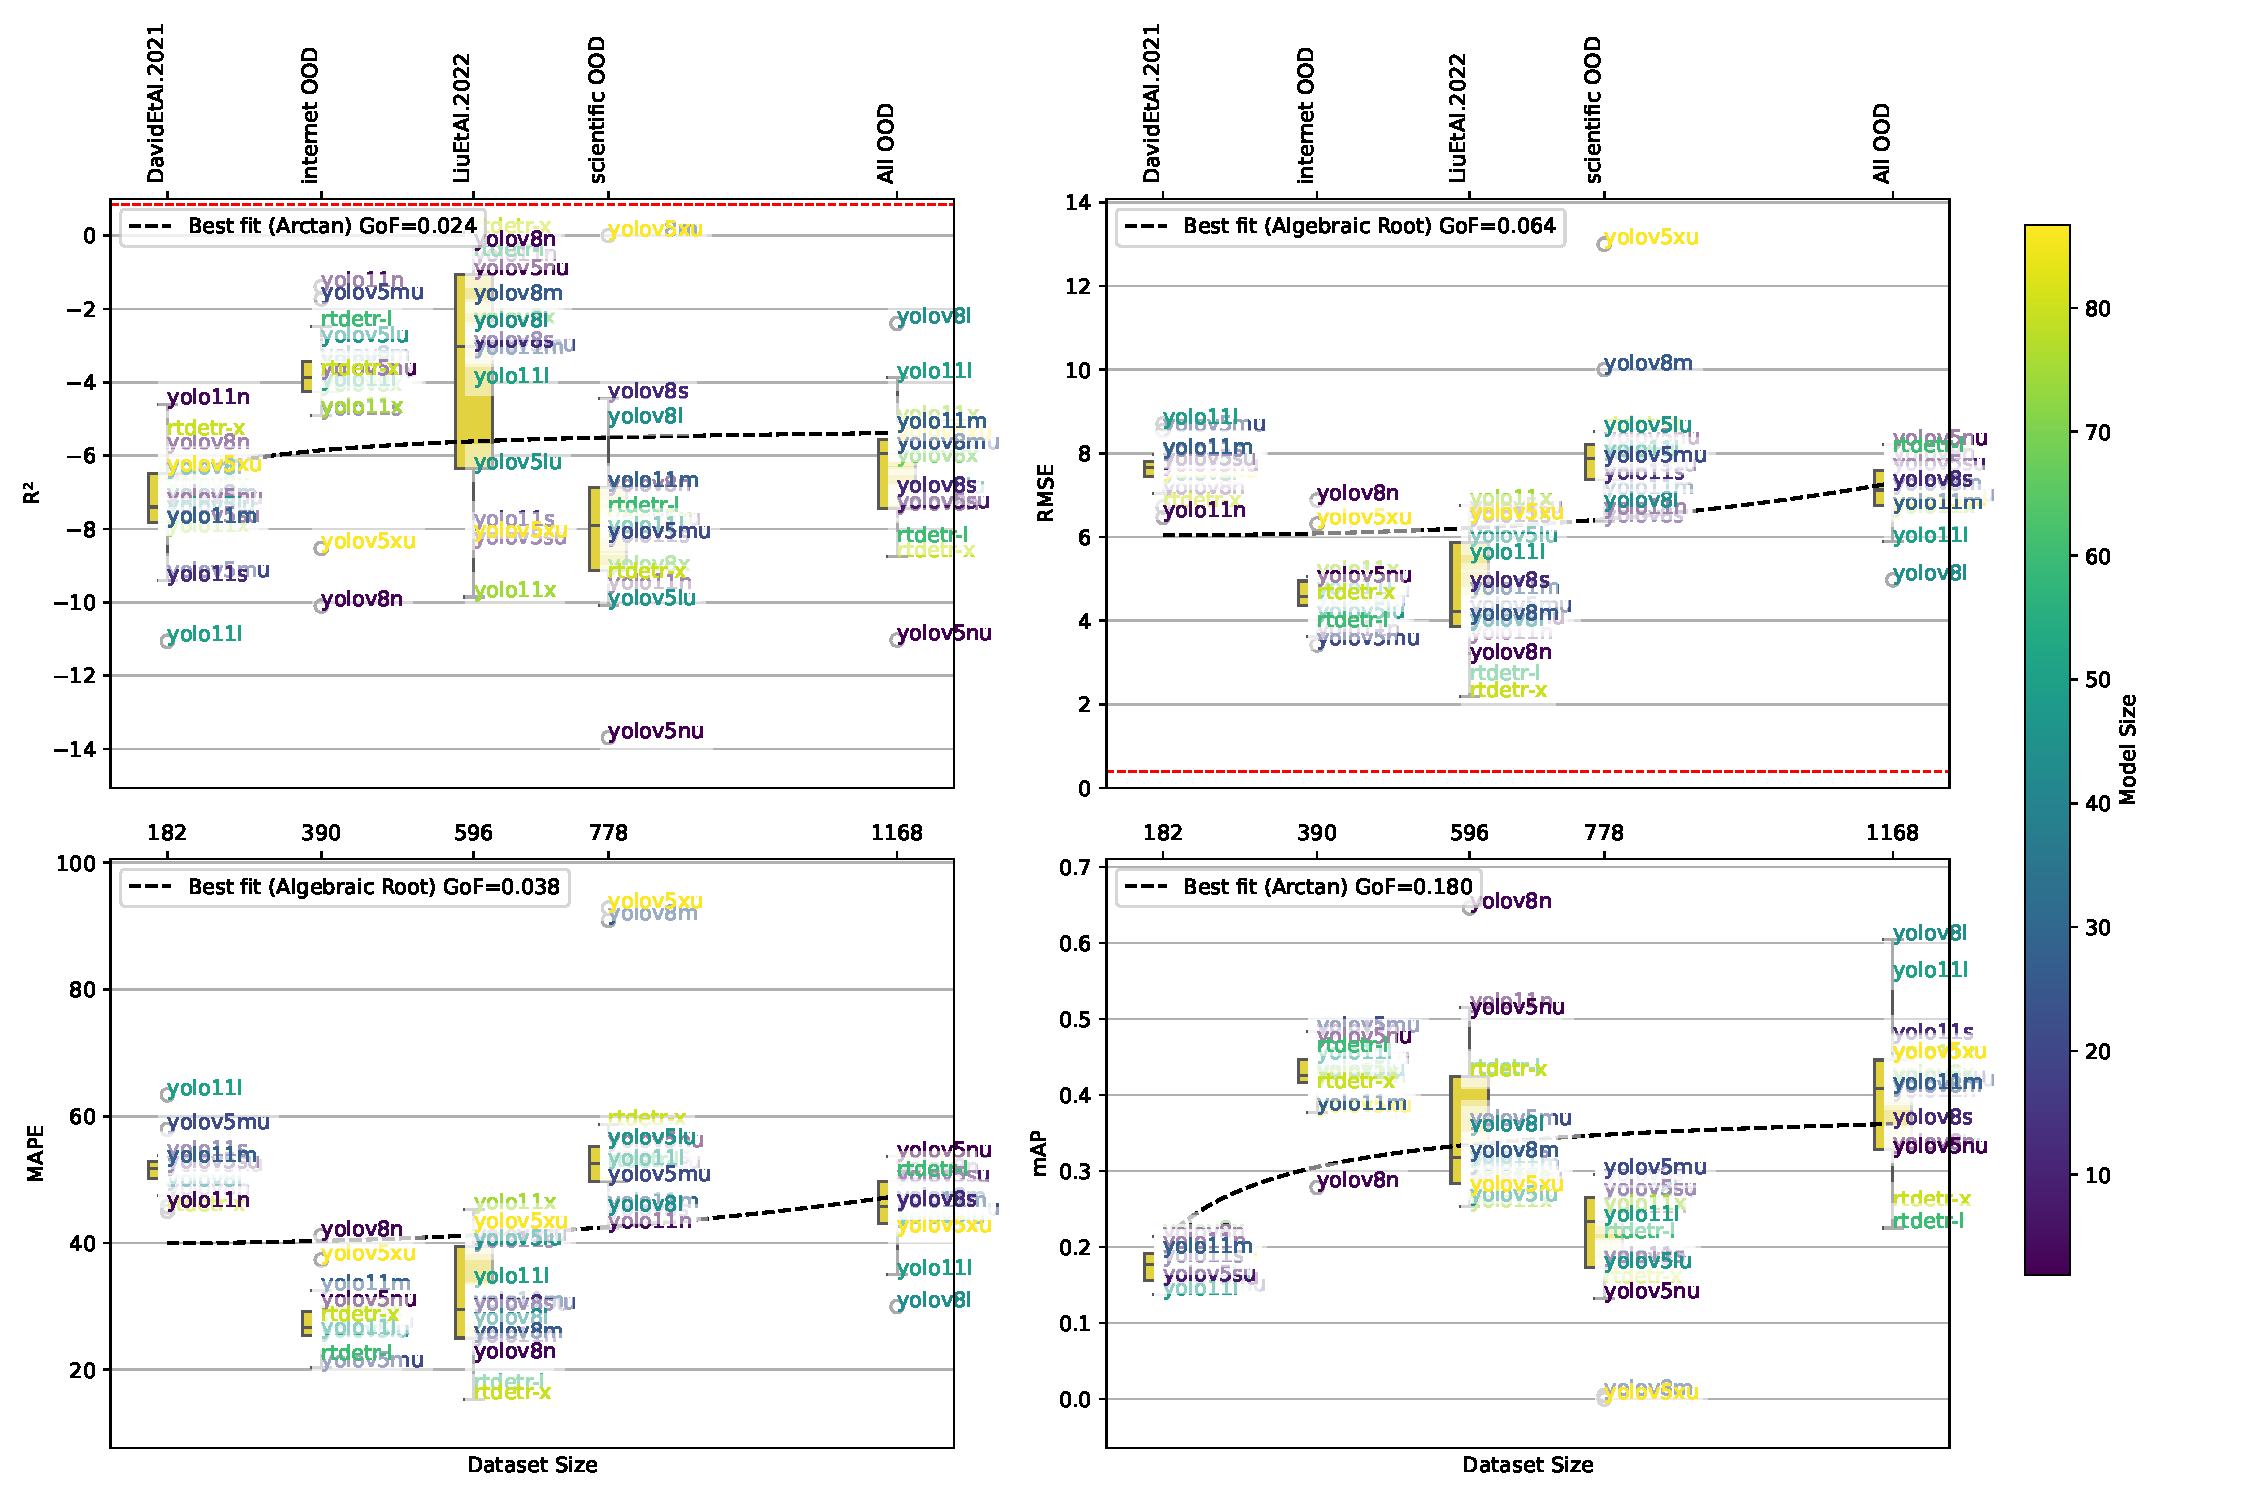
\includegraphics[width=\linewidth]{Plots/metrics_OOD_datasets.pdf}
\caption{The figure shows the performance of the many-shot object detection models 
trained on 
the different Out-of-Distribution (OOD) datasets. The~subplots represent four different metrics: 
R², $RMSE$, MAPE, and~$mAP$, respectively, at the right top, left top, left bottom, and~right bottom.
Each subplot contains the boxplots
positioned at the corresponding dataset size values and indicating the distribution of
all the model prediction metric values for each dataset.
Benchmark thresholds are indicated with red 
dashed horizontal lines for R² (0.85) and $RMSE$ (0.39). Best fit lines for each metric are 
plotted using different fitting functions, 
indicated with black dashed lines. $GoF$ values and best model are shown in the
legend.
A secondary x-axis at the top of each subplot 
shows the dataset names corresponding to the dataset sizes.}
\label{fig:metrics_OOD_datasets}
\end{figure}
\end{landscape}

\subsubsection{ID~Training}

The relationship between ID training dataset size and model performance was evaluated 
for all model architectures and sizes, as shown in Figures~\ref{fig:dataset_size_vs_performance_cnn} and~\ref{fig:dataset_size_vs_performance_transformer}. 
The dataset quality was tested later, taking the combination of model architecture, model size, and
training dataset size that achieved the benchmark and retraining that model while reducing the amount of
annotations for each tile. 
The $R^2$ values of the counting and the $mAP$ values for all models were regressed 
against the dataset size using a logarithmic, root, or arctan model. The~best fitting
within them was selected for each model and metric and the $GoF$ was calculated.
A high $GoF$ value indicates that model performance is highly predictable by dataset size. 
Conversely, a~poor $GoF$ could indicate that other variables play a more important 
role in determining model performance, or~that the chosen dataset size interval is 
too narrow to achieve a good~fit.

For the combinations of model-architecture/dataset-size that achieved the benchmark,
the minimum dataset quality required to achieve the benchmark was evaluated, as
shown in Figure~\ref{fig:dataset_quality}. The~minimum dataset quality was determined by identifying 
the quality percentage where both the empirical model prediction and the entire confidence interval 
of the performance metrics remained above the benchmark~threshold.

\begin{landscape}
\begin{figure}
 \begin{adjustwidth}{-\extralength}{0cm}
  \centering
  \subfloat[\centering]{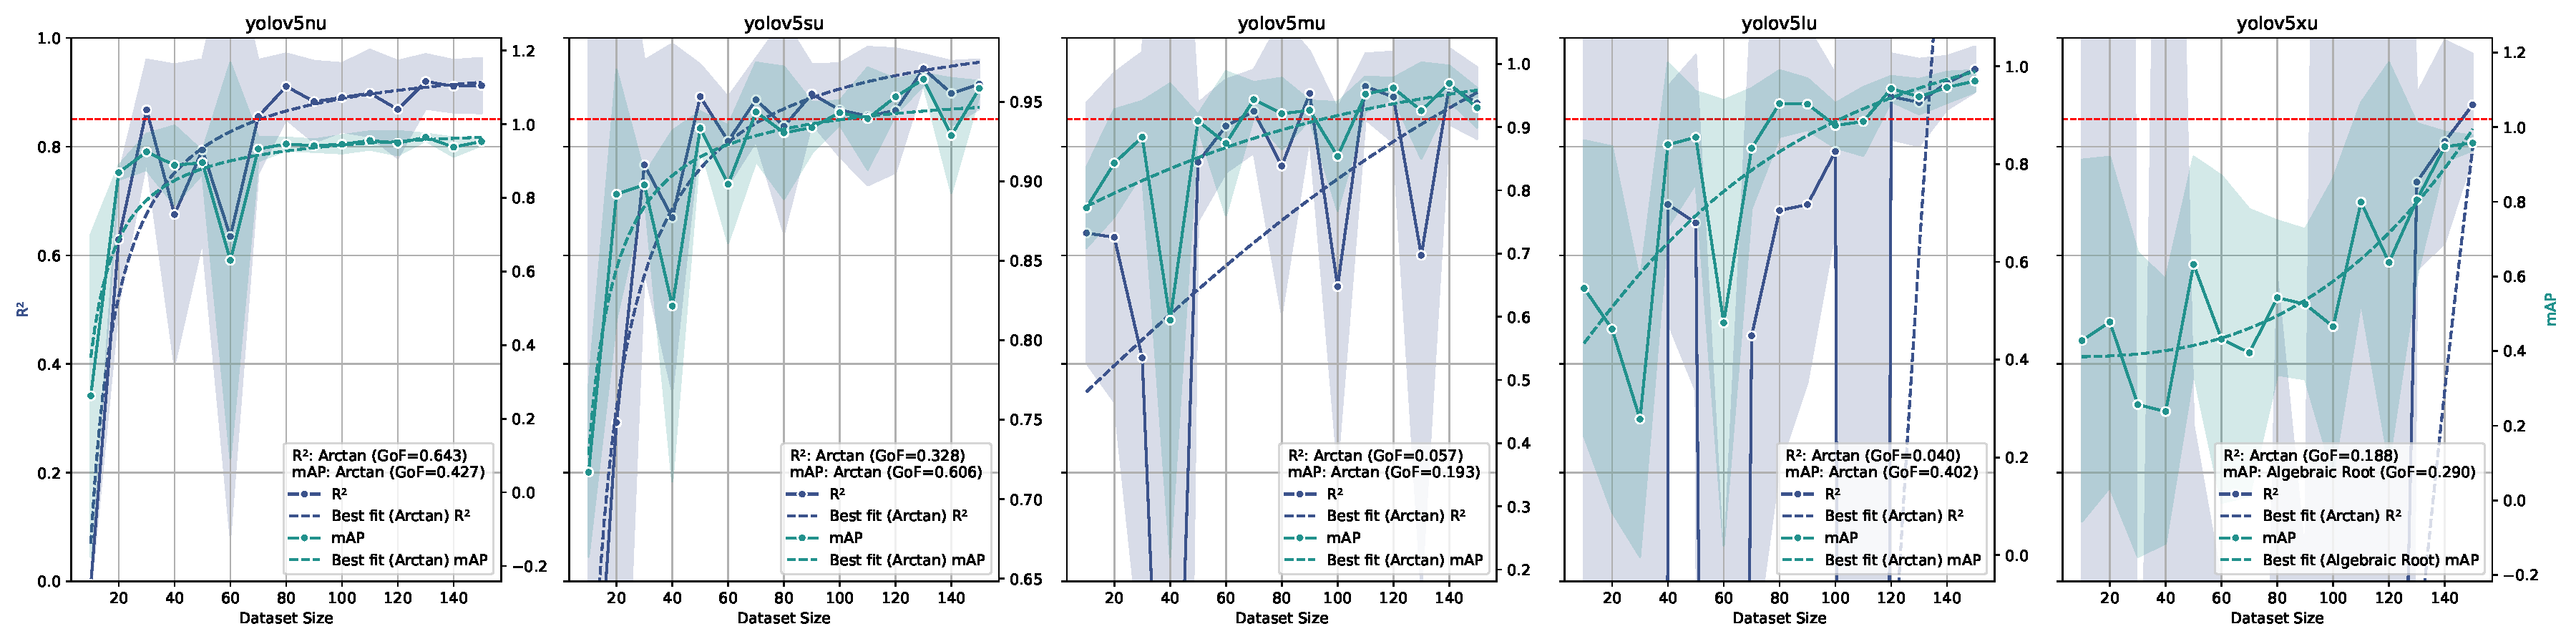
\includegraphics[width=22cm]{Plots/r2_ap_vs_dataset_size_yolov5.pdf}}\\
  \subfloat[\centering]{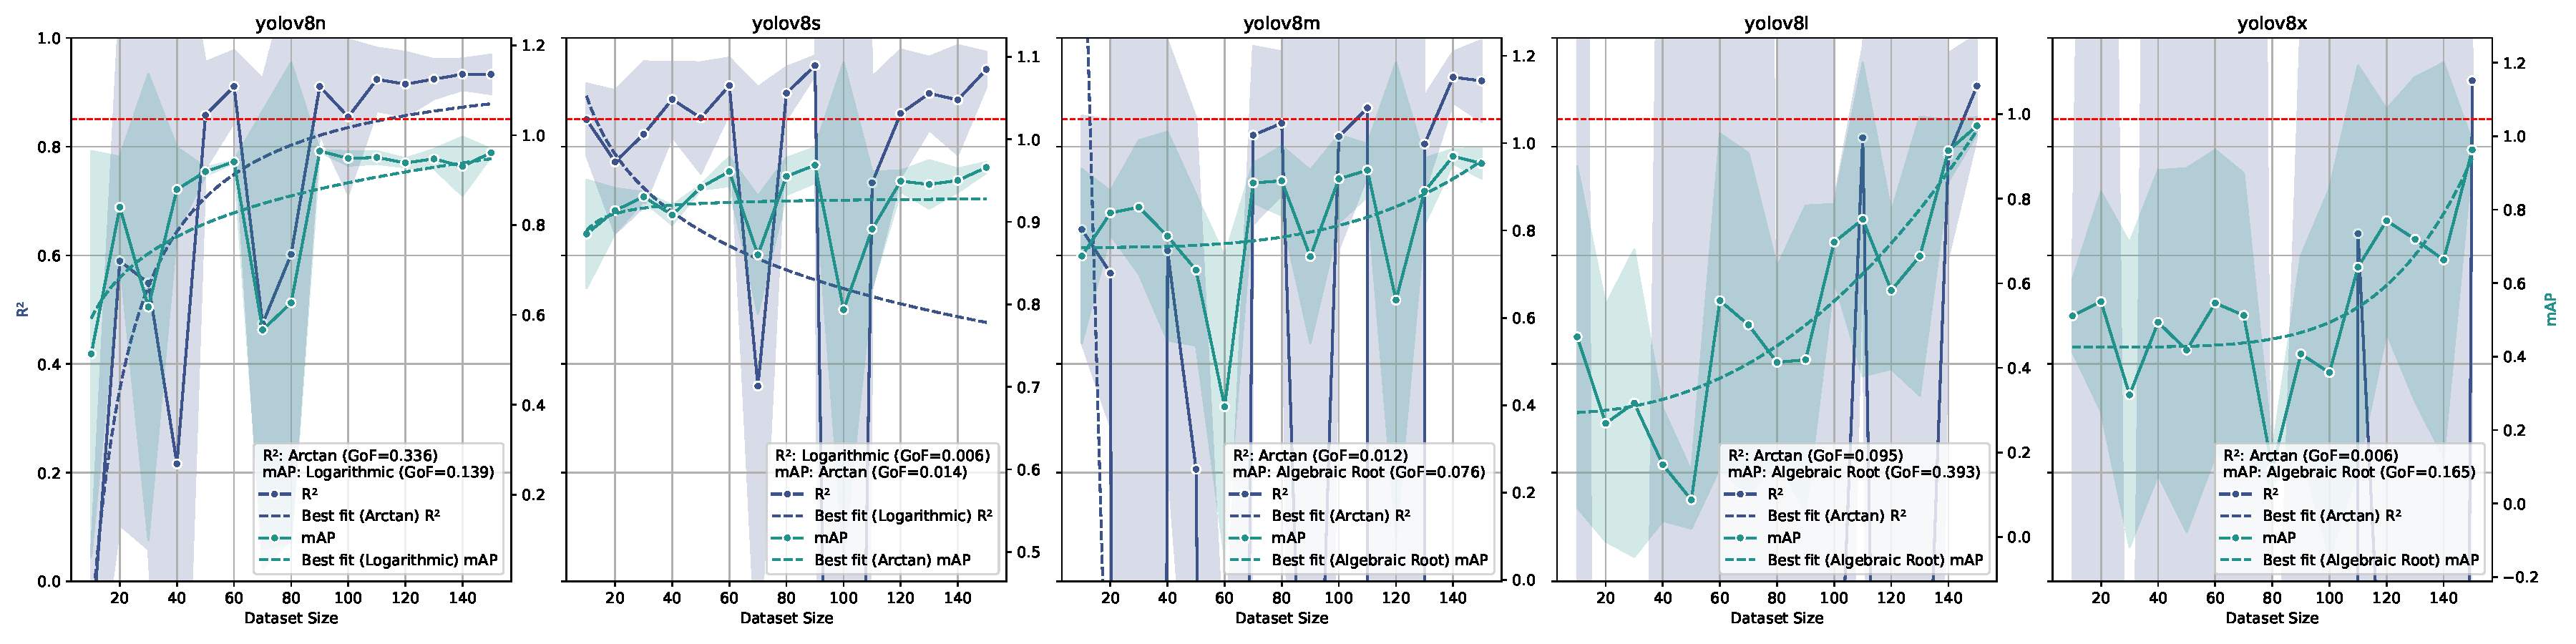
\includegraphics[width=22cm]{Plots/r2_ap_vs_dataset_size_yolov8.pdf}}\\
\end{adjustwidth}
 \caption{Relationship between dataset size and model performance 
  for CNN-based object detection models (YOLOv5 (\textbf{a}) and YOLOv8 (\textbf{b})) trained and tested on ID datasets. 
  On the same line, each subplot represents a different parameters size of the model,
  increasing from the left to the right. The~x-axis represents the dataset size, while
  the left and right y-axis represents the $R^2$ and $mAP$ values, respectively. 
  The solid lines represent the mean values, while the dashed lines indicate the logarithmic fit.
  The shaded area around the solid lines represents the confidence interval (standard
  deviation) of $R^2$ or $mAP$.
  The red dashed horizontal line represents the benchmark $R^2$ value of 0.85. The~combined
  legend in the lower right corner of each subplot shows the Goodness of Fit ($GoF$) for both $R^2$
  and $mAP$.}
  \label{fig:dataset_size_vs_performance_cnn}
\end{figure}
\end{landscape}

\begin{landscape}
\begin{figure}
 \begin{adjustwidth}{-\extralength}{0cm}
  \centering
  \subfloat[\centering]{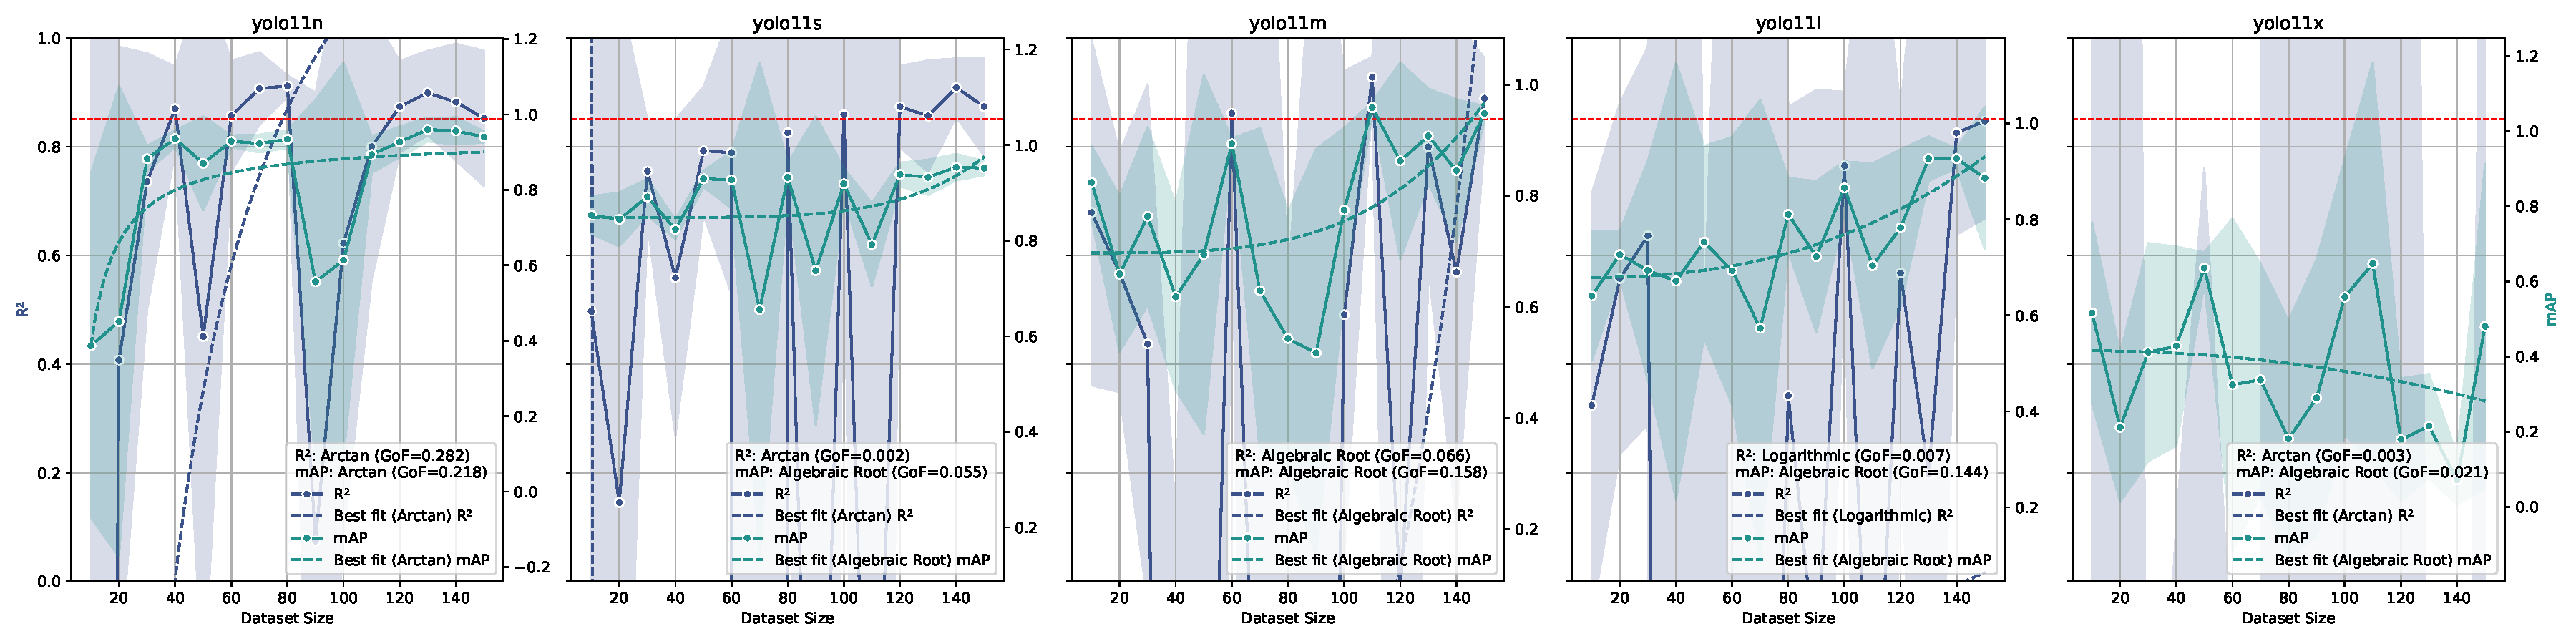
\includegraphics[width=22cm]{Plots/r2_ap_vs_dataset_size_yolo11.pdf}}\\
  \subfloat[\centering]{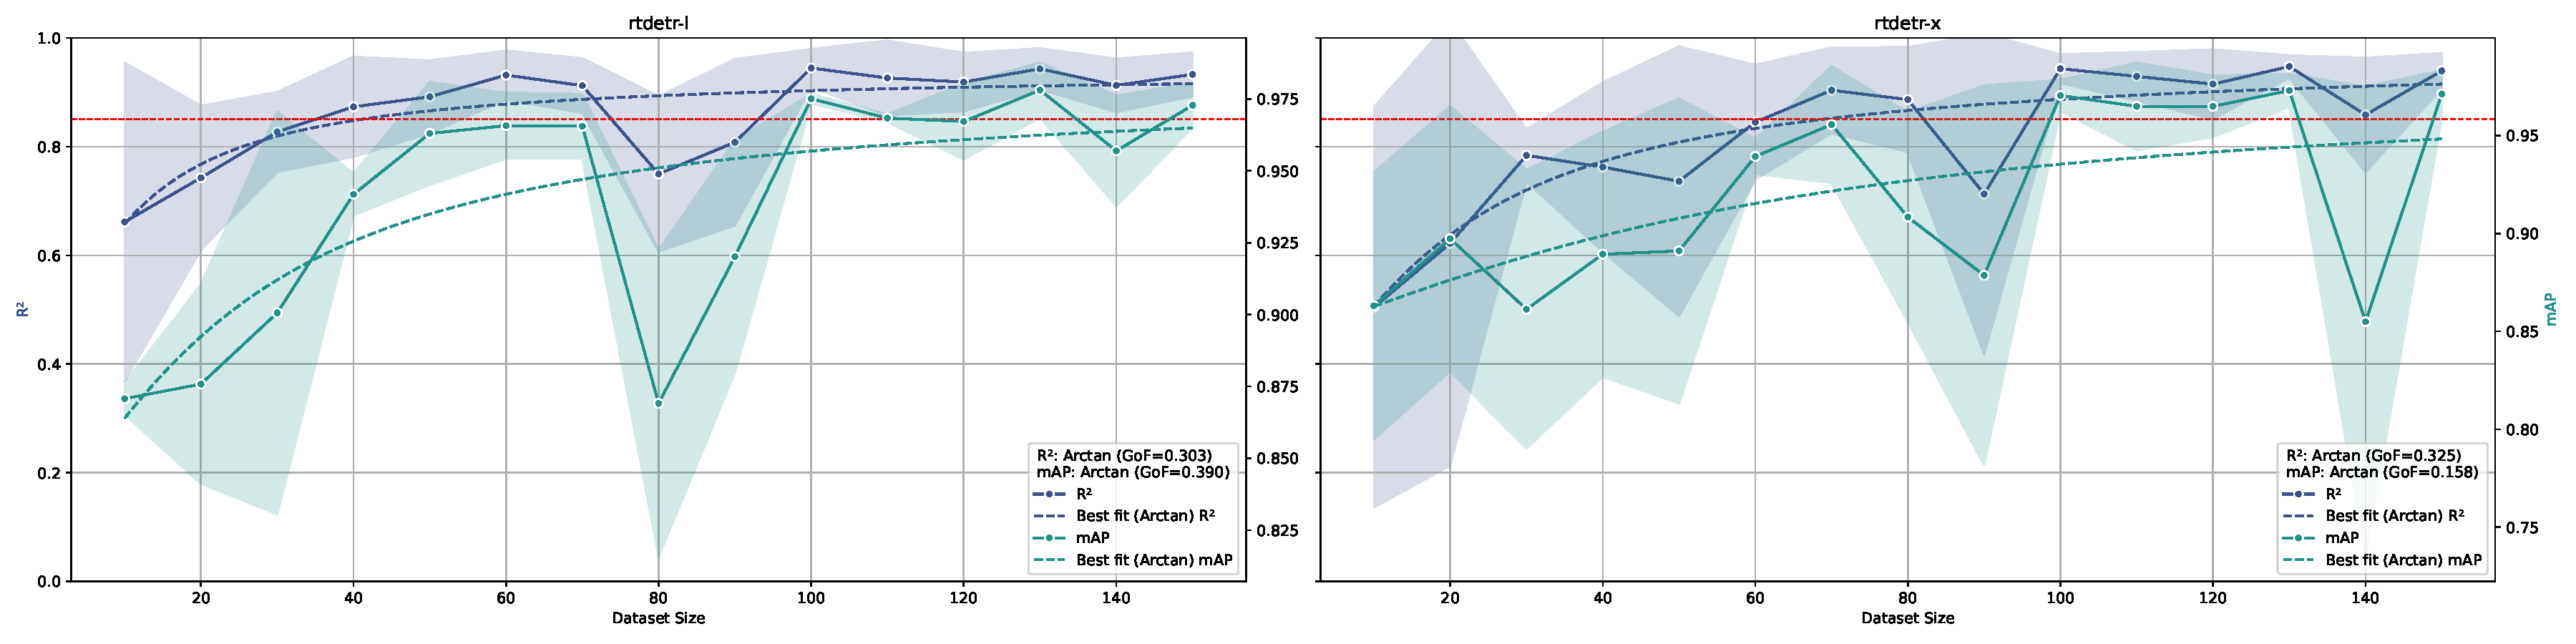
\includegraphics[width=22cm]{Plots/r2_ap_vs_dataset_size_rtdetr.pdf}}\\
\end{adjustwidth}
 \caption{Relationship between dataset size and model performance 
  for Transformer-mixed object detection models (YOLO11 (\textbf{a}) and RT-DETR (\textbf{b})) trained and tested on ID datasets. 
  On the same line, each subplot represents a different parameters size of the model,
  increasing from the left to the right. The~x-axis represents the dataset size, while
  the left and right y-axis represents the $R^2$ and $mAP$ values, respectively. 
  The solid lines represent the mean values, while the dashed lines indicate the logarithmic fit.
  The shaded area around the solid lines represents the confidence interval (standard
  deviation) of $R^2$ or $mAP$.
  The red dashed horizontal line represents the benchmark $R^2$ value of 0.85. The~combined
  legend in the lower right corner of each subplot shows the Goodness of Fit ($GoF$) for both $R^2$
  and $mAP$.}
  \label{fig:dataset_size_vs_performance_transformer}
\end{figure}
\end{landscape}

Within YOLO models, YOLOv5n, YOLOv5s, and YOLOv8n achieve the benchmark $R^2$ 
value of 0.85 with 130, 130, and 110 samples, respectively, considering the dataset
sizes where all three model performances were above 0.85 $R^2$ and the logarithmic
model predicted over-benchmark values for that dataset size.
RT-DETR L and RT-DETR X achieve the benchmark $R^2$ value of 0.85 with 60 and 100 samples,
respectively, with~the same assumptions as for the YOLO models.
For these models, the $GoF$ was above 0.3, while for the models that did
not reach the benchmark $R^2$ value the $GoF$ was always below this value.
The $mAP$ seems to follow the same trend as the $R^2$ values.
All the models show a clear trend of increasing $R^2$ and $mAP$
values as the dataset size increases, as~expected.
It is also clear that increasing the number of parameters and model complexity for
mostly CNN-like models (YOLOs) leads to increasing need for dataset size.
For the mostly transformer-like models (RT-DETRs), it is not that clear, also because of
the low amount of model parameter sizes tested.
The confidence interval reduction as a function of the dataset size indicates that 
variability in performance decreases significantly as dataset size increases for 
all models.
Taking into account the dataset quality in the same way as done for the dataset size,
both quality tests and quality models achieved the benchmark, with 85\%, 90\%, 85\%, and
65\% of the original dataset quality for YOLOv5n, YOLOv5s, YOLOv8n, and RT-DETR X, respectively.
RT-DETR L did not achieve the benchmark for any dataset quality reduction tested.
Overall, RT-DETR performed best in terms of both dataset size and quality. 
The best performance in terms of dataset size was achieved with RT-DETR trained 
on 60 images (see prediction examples in Figure~\ref{fig:annotations_many-shots_size}), while the best performance in 
terms of dataset quality 
was achieved with RT-DETR trained on 100 images with a 35\% reduction in quality
(see Figure~\ref{fig:annotations_many-shots_quality} for prediction examples).

\begin{landscape}
\begin{figure}
  \begin{adjustwidth}{-\extralength}{0cm}
  \centering
  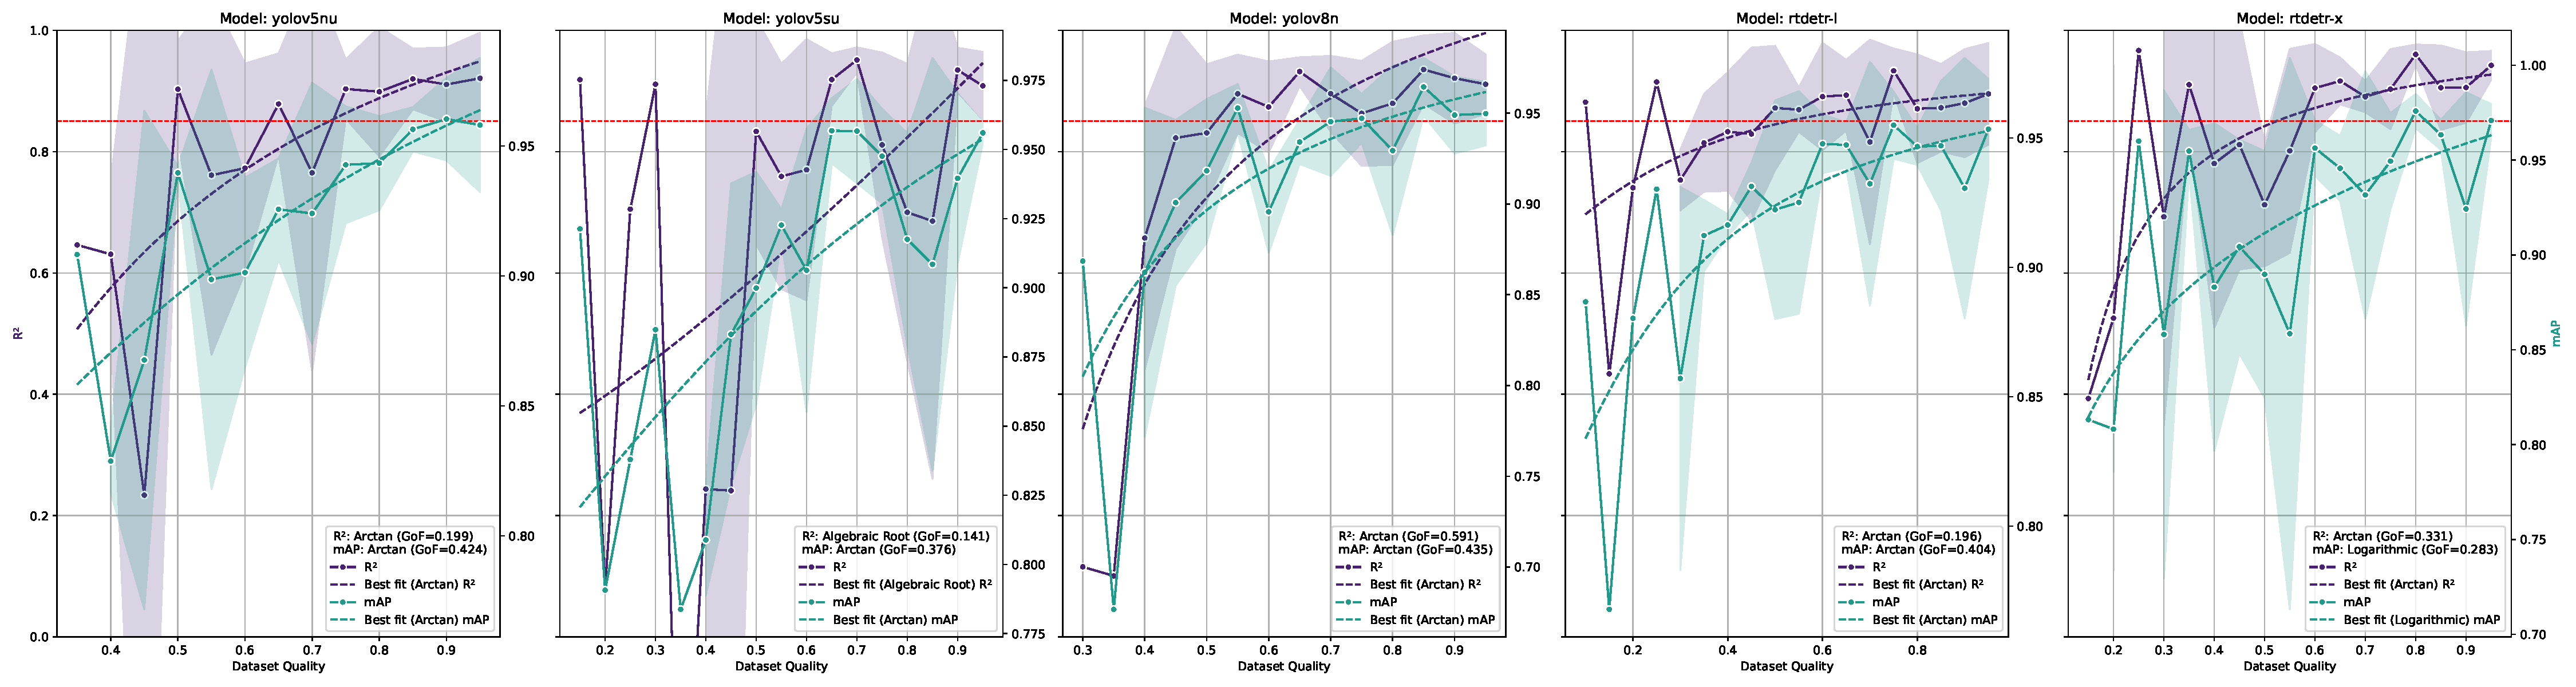
\includegraphics[width=22cm]{Plots/r2_ap_vs_dataset_quality.pdf}
  \end{adjustwidth}   
   \caption{Relationship between dataset quality and model performance for all object detection models
  that achieved the benchmark. The~x-axis represents the dataset quality, while 
  the left y-axis represents the $R^2$ values.
  The red dashed horizontal line represents the benchmark $R^2$ value of 0.85. The~  legend in the lower right corner of the subplot shows the Goodness of Fit ($GoF$) for $R^2$.}
  \label{fig:dataset_quality}
\end{figure}
\end{landscape}

\begin{landscape}
\begin{figure}
  \begin{adjustwidth}{-\extralength}{0cm}
  \centering
  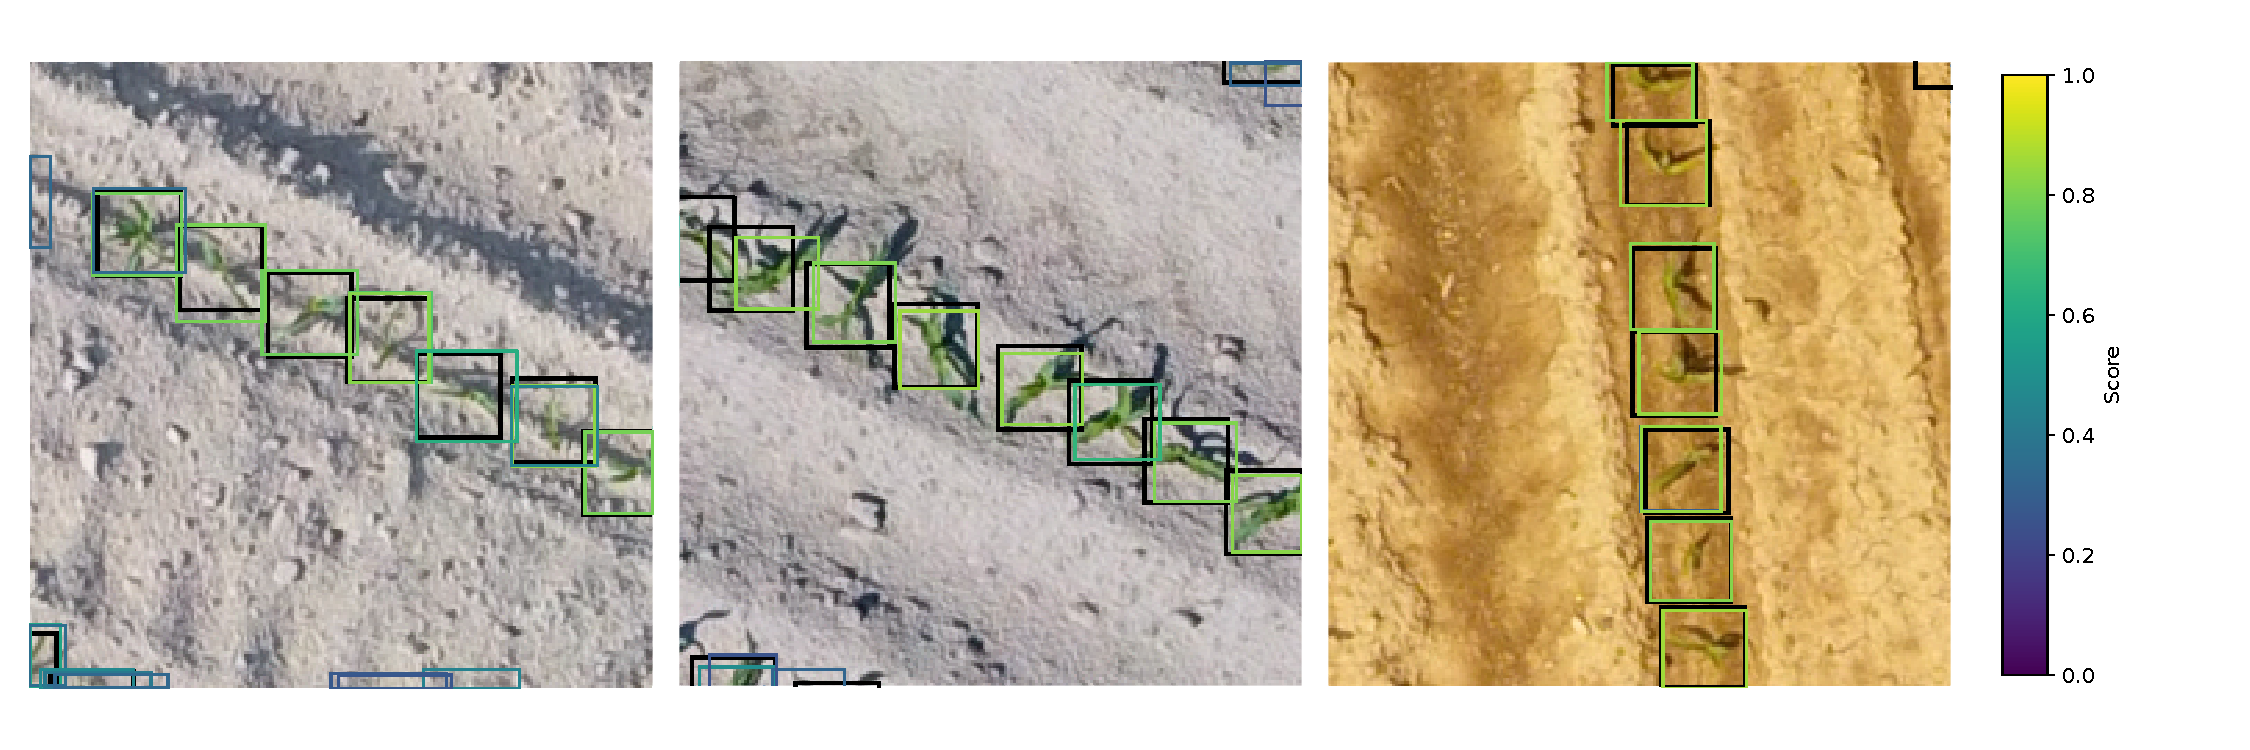
\includegraphics[width=22cm]{Plots/many_shot_size_annotations.pdf}
  \end{adjustwidth}
  \vspace{-12pt}\caption{Predictions from the RT-DETR L trained on 60 images.
  From the left hand side to the right hand side, the~images show the
  1, 2, and 3 ID test dataset tile examples.
  The predicted bounding boxes in the images are the ones before 
  non-maximum suppression and threshold.
   Black bounding boxes are the ground truth annotations, while the bounding boxes 
   in the viridis color scale are the model~predictions.}
  \label{fig:annotations_many-shots_size}
\end{figure}
\end{landscape}

\begin{landscape}
\begin{figure}
  \begin{adjustwidth}{-\extralength}{0cm}
  \centering
  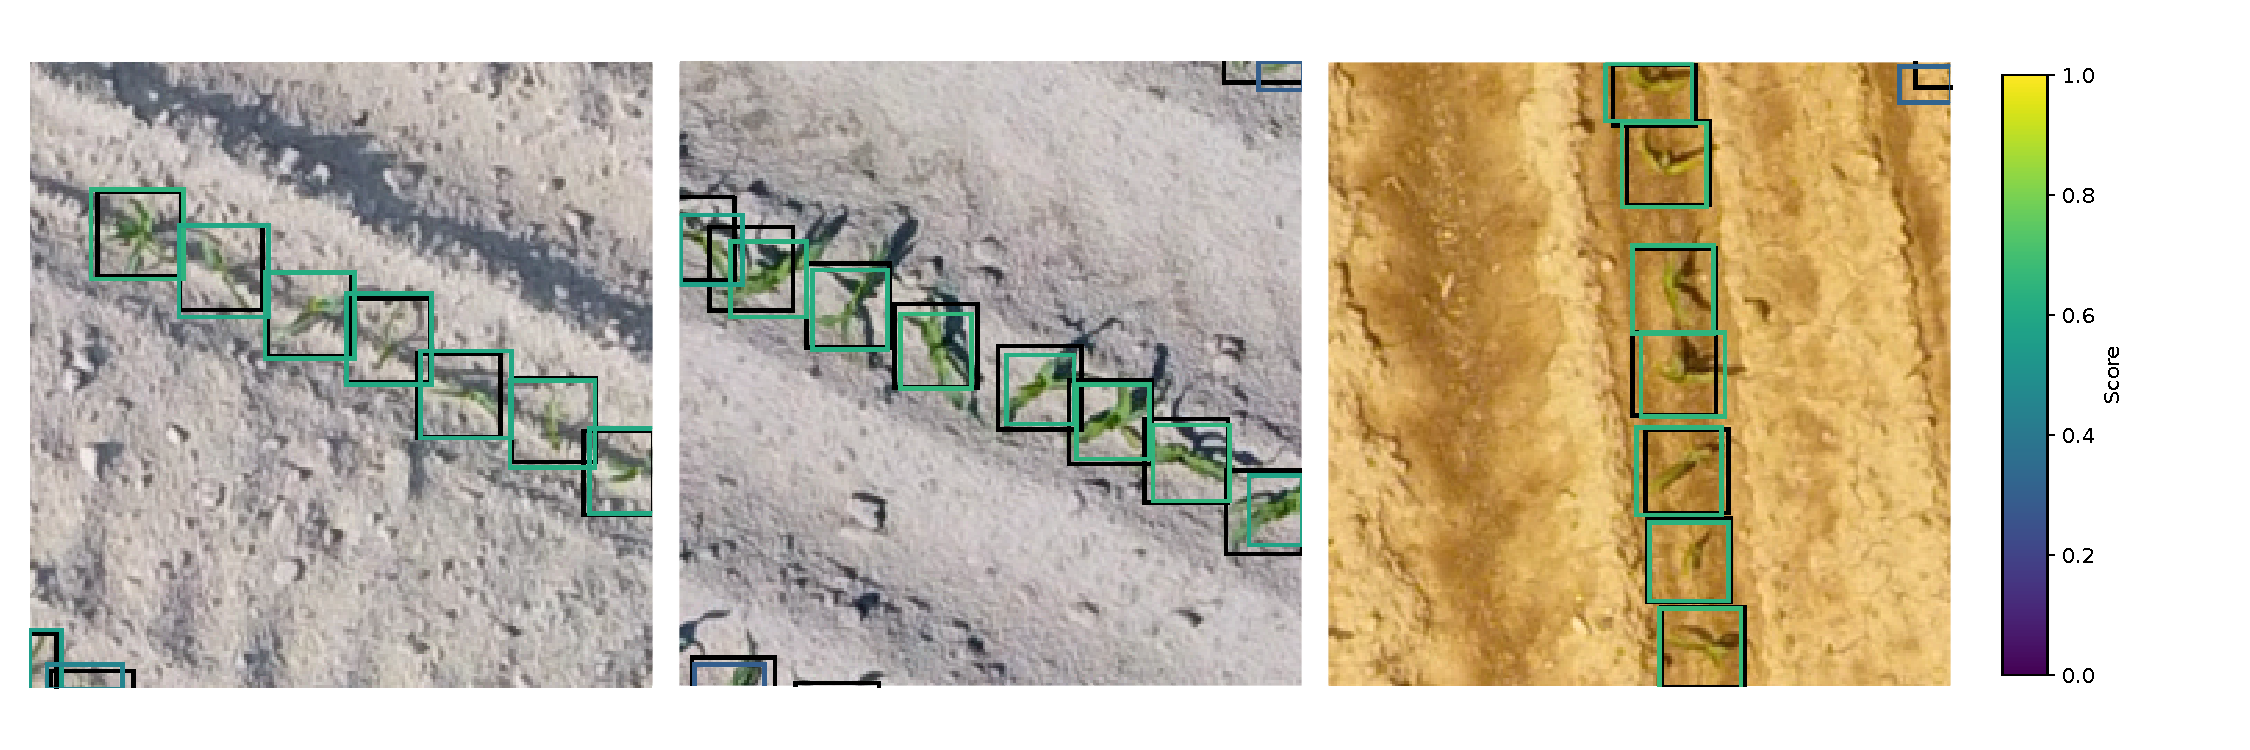
\includegraphics[width=22cm]{Plots/many_shot_quality_annotations.pdf}
  \end{adjustwidth}
  \vspace{-12pt}\caption{Predictions from the RT-DETR X trained on 100 images with a reduction 
  in quality of 35\%.
  From the left hand side to the right hand side, the~images show the
  1, 2, and 3 ID test dataset tile examples.
  The predicted bounding boxes in the images are the ones before 
  non-maximum suppression and threshold.
   Black bounding boxes are the ground truth annotations, while the bounding boxes 
   in the viridis color scale are the model~predictions.}
  \label{fig:annotations_many-shots_quality}
\end{figure}
\end{landscape}

\subsection{Few-Shot Object~Detectors}

The few-shot models were evaluated against the established benchmarks ($R^2$ of 0.85 and $RMSE$ of 0.39) 
using the metrics $R^2$ and $RMSE$; however, none of the models reached these~benchmarks.

The best result achieved by the CD-ViTO model was an $RMSE$ of 3.9 with ViT-B backbone and 
50 shots to build the prototypes, which is substantially worse than the benchmark value of 0.39 (10 times higher). 
This corresponds to a $MAPE$ on counting of about 25\% 
and a $mAP$ of about 0.5, as shown in Figure~\ref{fig:shots_vs_performance}.
It corresponds roughly to a miscounted plant over four as it is visible, looking to
some predictions of this model in Figure~\ref{fig:annotations_few-shot}.
The models fitted on metrics show a reliable $GoF$ for all
the metrics, indicating that the model performance is highly predictable by the number of shots.
These also show that any CD-ViTO size model would not achieve the
benchmark with any shot amount, even if the number of shots were increased beyond those~tested.

\subsection{Zero-Shot Object~Detectors}

Figure~\ref{fig:zeroshots_vs_performance} shows the relationship between the zero-shot 
model settings and model performance tested on ID testing datasets. Not all the 
model settings were able to predict the whole testing dataset. For~example, the~
owlv2-base-patch16-finetuned model was not able to generate any prediction with 
any prompt for any image of the ID testing. A~dataset size relationship with metrics 
could not be established because zero-shot models do not require fine-tuning training 
data.
None of the zero-shot model settings reached the benchmark. This is particularly true for the 
$R^2$ values, which were always below 0, indicating poor predictive performance. The~
$RMSE$ values ranged from approximately 5 to 25, significantly higher than those 
observed in the many-shot and few-shot models. Additionally, $MAPE$ values were 
also considerably elevated, ranging from around 40 to 140. Furthermore, the~
$mAP$ values were lower than those of the many and few-shot models for all model 
settings, except~for the owlv2-large-patch14-finetuned model, for~which very few 
images were successfully predicted with an 
$mAP$ comparable to that of the best few-shot model (50-shots ViT-B backbone).
Some rare cases of good predictions were even more accurate than the few-shot best performance, 
as shown in Figure~\ref{fig:annotations_zero-shot}.

\begin{landscape}
\begin{figure}
  \begin{adjustwidth}{-\extralength}{0cm}
   \centering
  \subfloat[\centering]{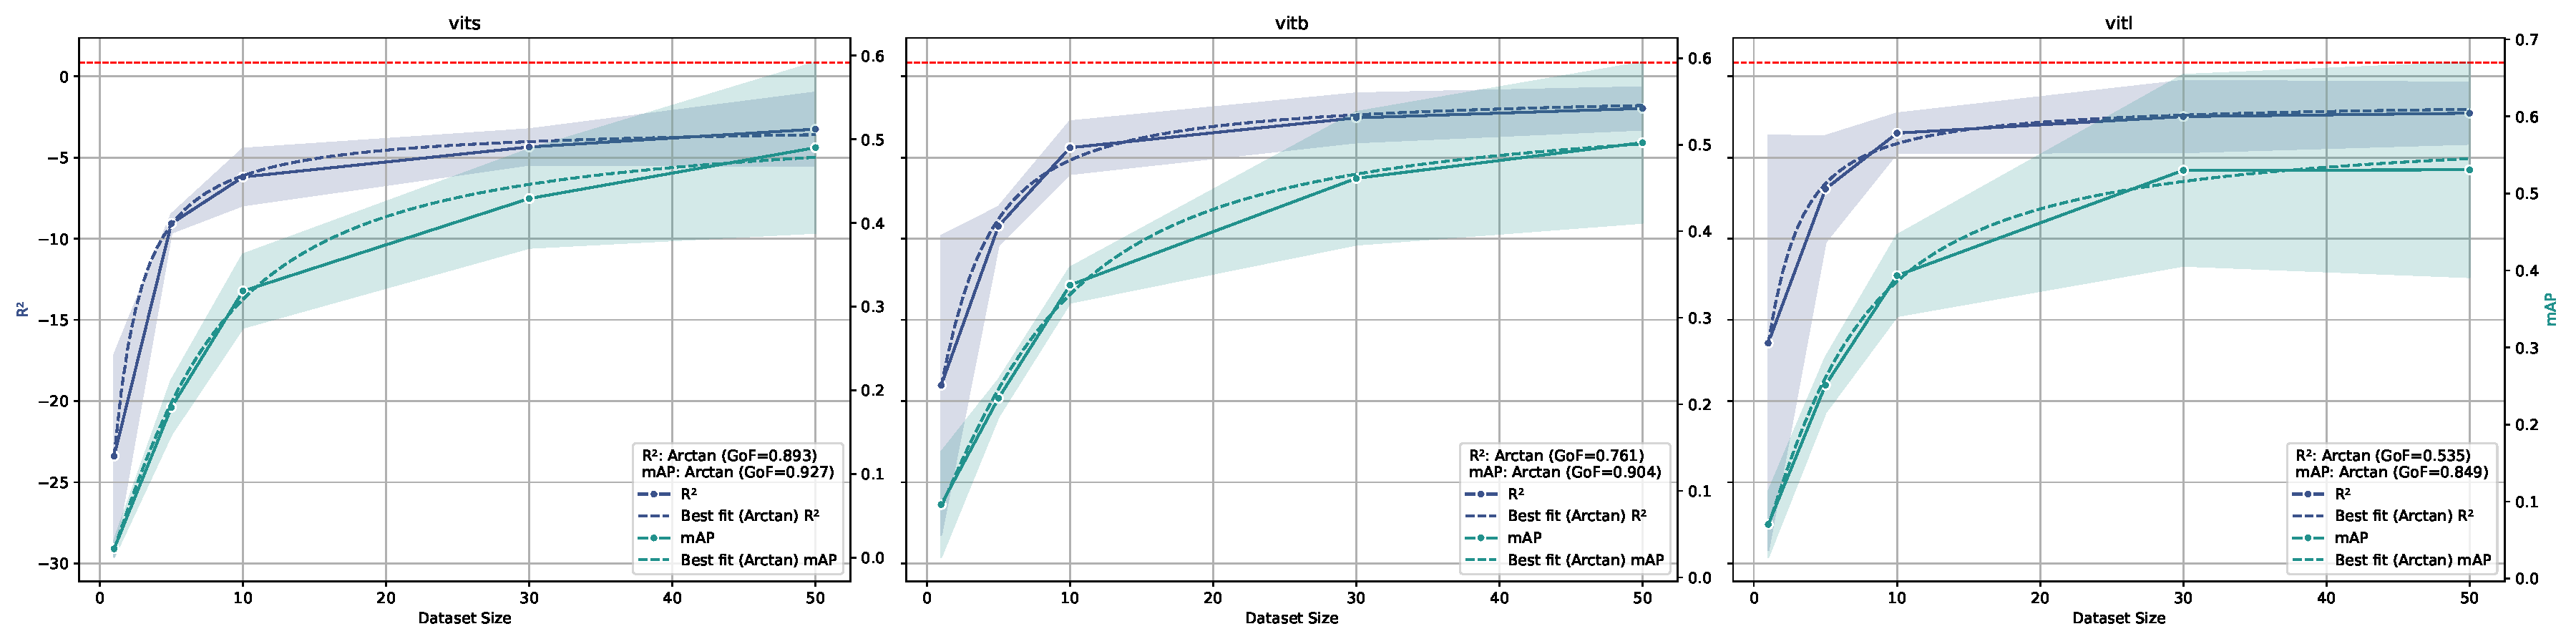
\includegraphics[width=22cm]{Plots/r2_ap_vs_shots_cdvito.pdf}}\\
  \subfloat[\centering]{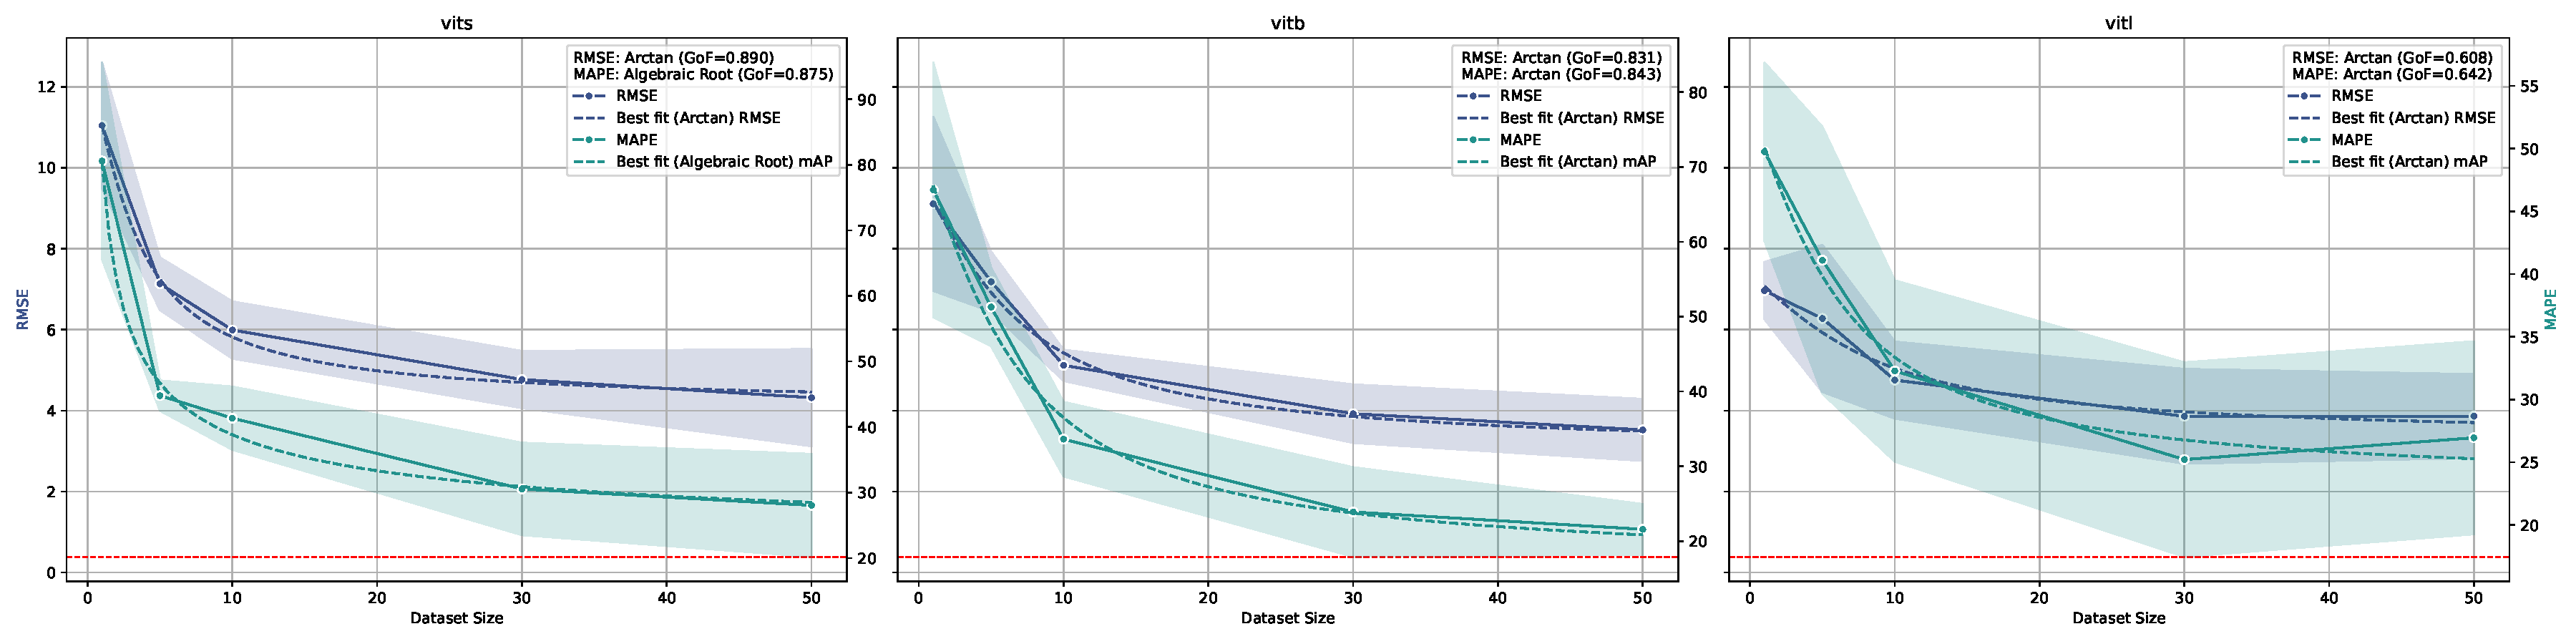
\includegraphics[width=22cm]{Plots/rmse_ap_vs_shots_cdvito.pdf}}\\
  \end{adjustwidth}
  \caption{The figure shows the relationship between shots and model performance
  for the CD-ViTO model trained and tested on ID datasets.
  The x-axis represents the number of shots.  The solid lines represent the mean values, while the dashed lines indicate the shot amount/metric 
  prediction model. The shaded area around the solid lines represents the confidence interval (standard deviation) of the metric.
  (\textbf{a}) The left and right y-axis represents the $R^2$ and $mAP$ values, respectively.
  The red dashed horizontal line represents the benchmark $R^2$ value of 0.85. The~combined
  legend in the lower right corner of each subplot shows the Goodness of Fit ($GoF$) for both $R^2$
  and $mAP$.
  (\textbf{b}) The left and right y-axis represents the $RMSE$ and $MAPE$ values respectively.
  The red dashed horizontal line represents the benchmark $RMSE$ value of 0.39. The~combined
  legend in the upper right corner of each subplot shows the Goodness of Fit ($GoF$) for both $RMSE$
  and MAPE.}
  \label{fig:shots_vs_performance}
\end{figure}
\end{landscape}

\begin{landscape}
\begin{figure}
  \begin{adjustwidth}{-\extralength}{0cm}
   \centering
  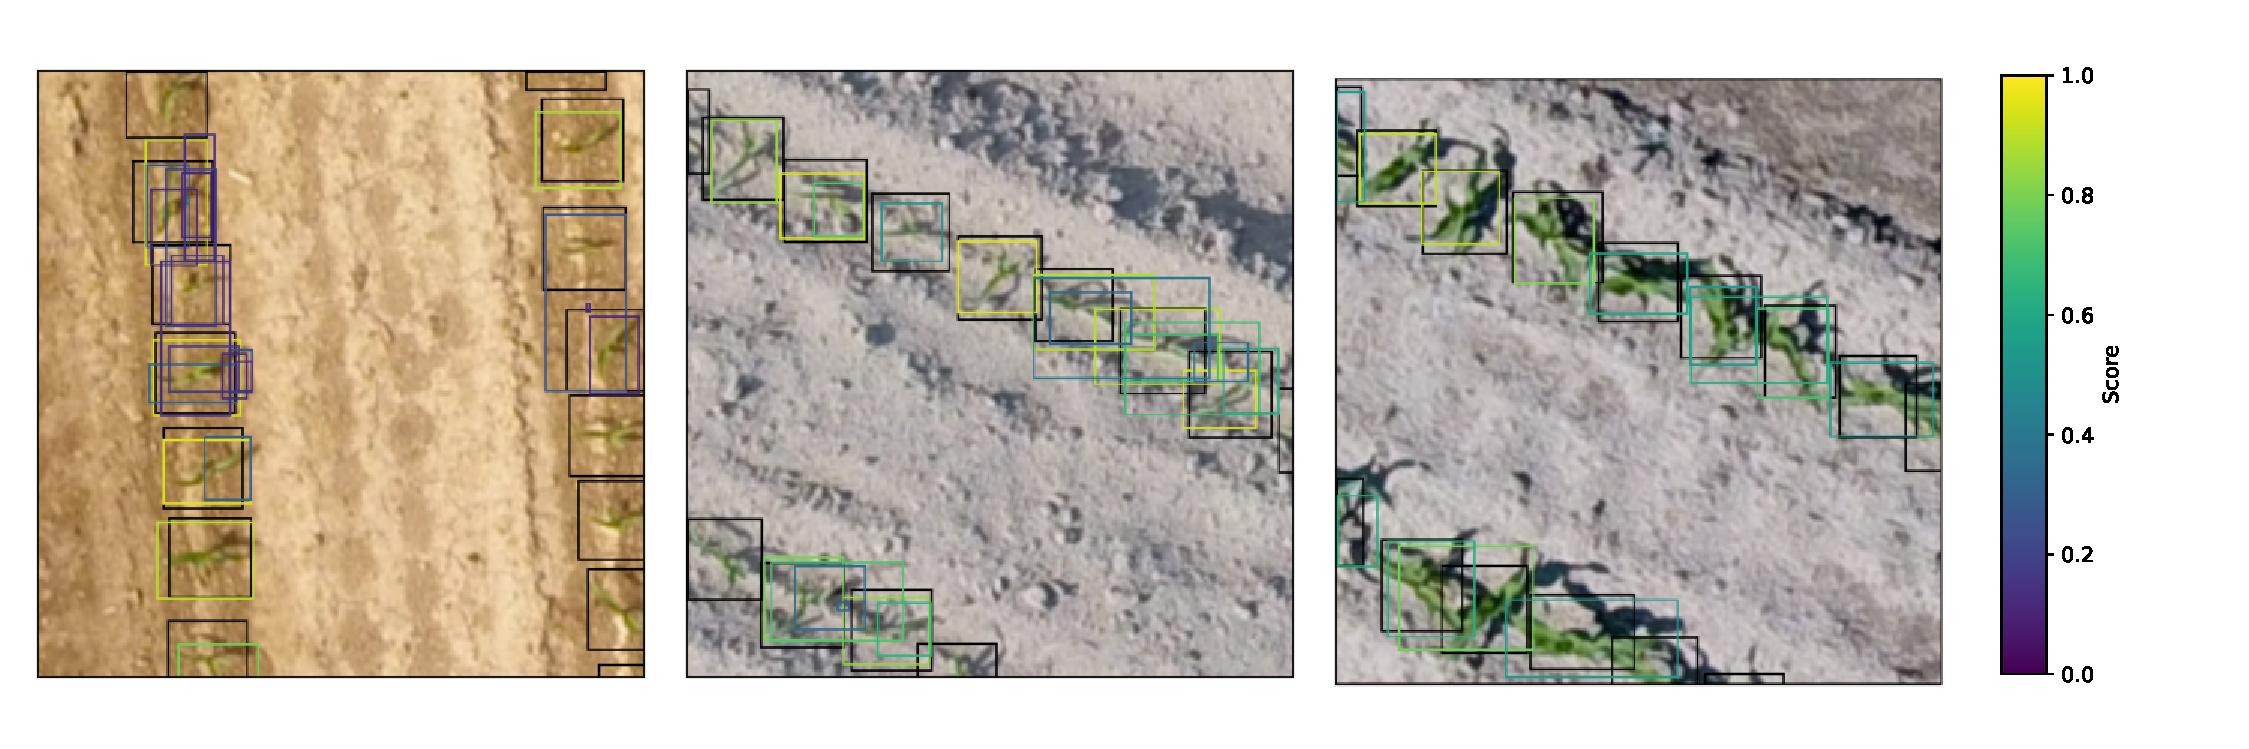
\includegraphics[width=22cm]{Plots/few_shot_annotations.pdf}
  \end{adjustwidth}
  \caption{The 50 shot CD-ViTO with ViT-B backbone predictions on the 
  1, 2, and 3 ID test dataset tile examples, respectively, from the left hand side to the right.
  The predicted bounding boxes in the images are the ones before 
  non-maximum suppression and threshold.
   Black bounding boxes are the ground truth annotations, while the bounding boxes 
   in the viridis color scale are the \mbox{model predictions.}}
  \label{fig:annotations_few-shot}
\end{figure}
\end{landscape}


\begin{landscape}
\begin{figure}
 % \centering
  \begin{adjustwidth}{-\extralength}{0cm}
  \centering
  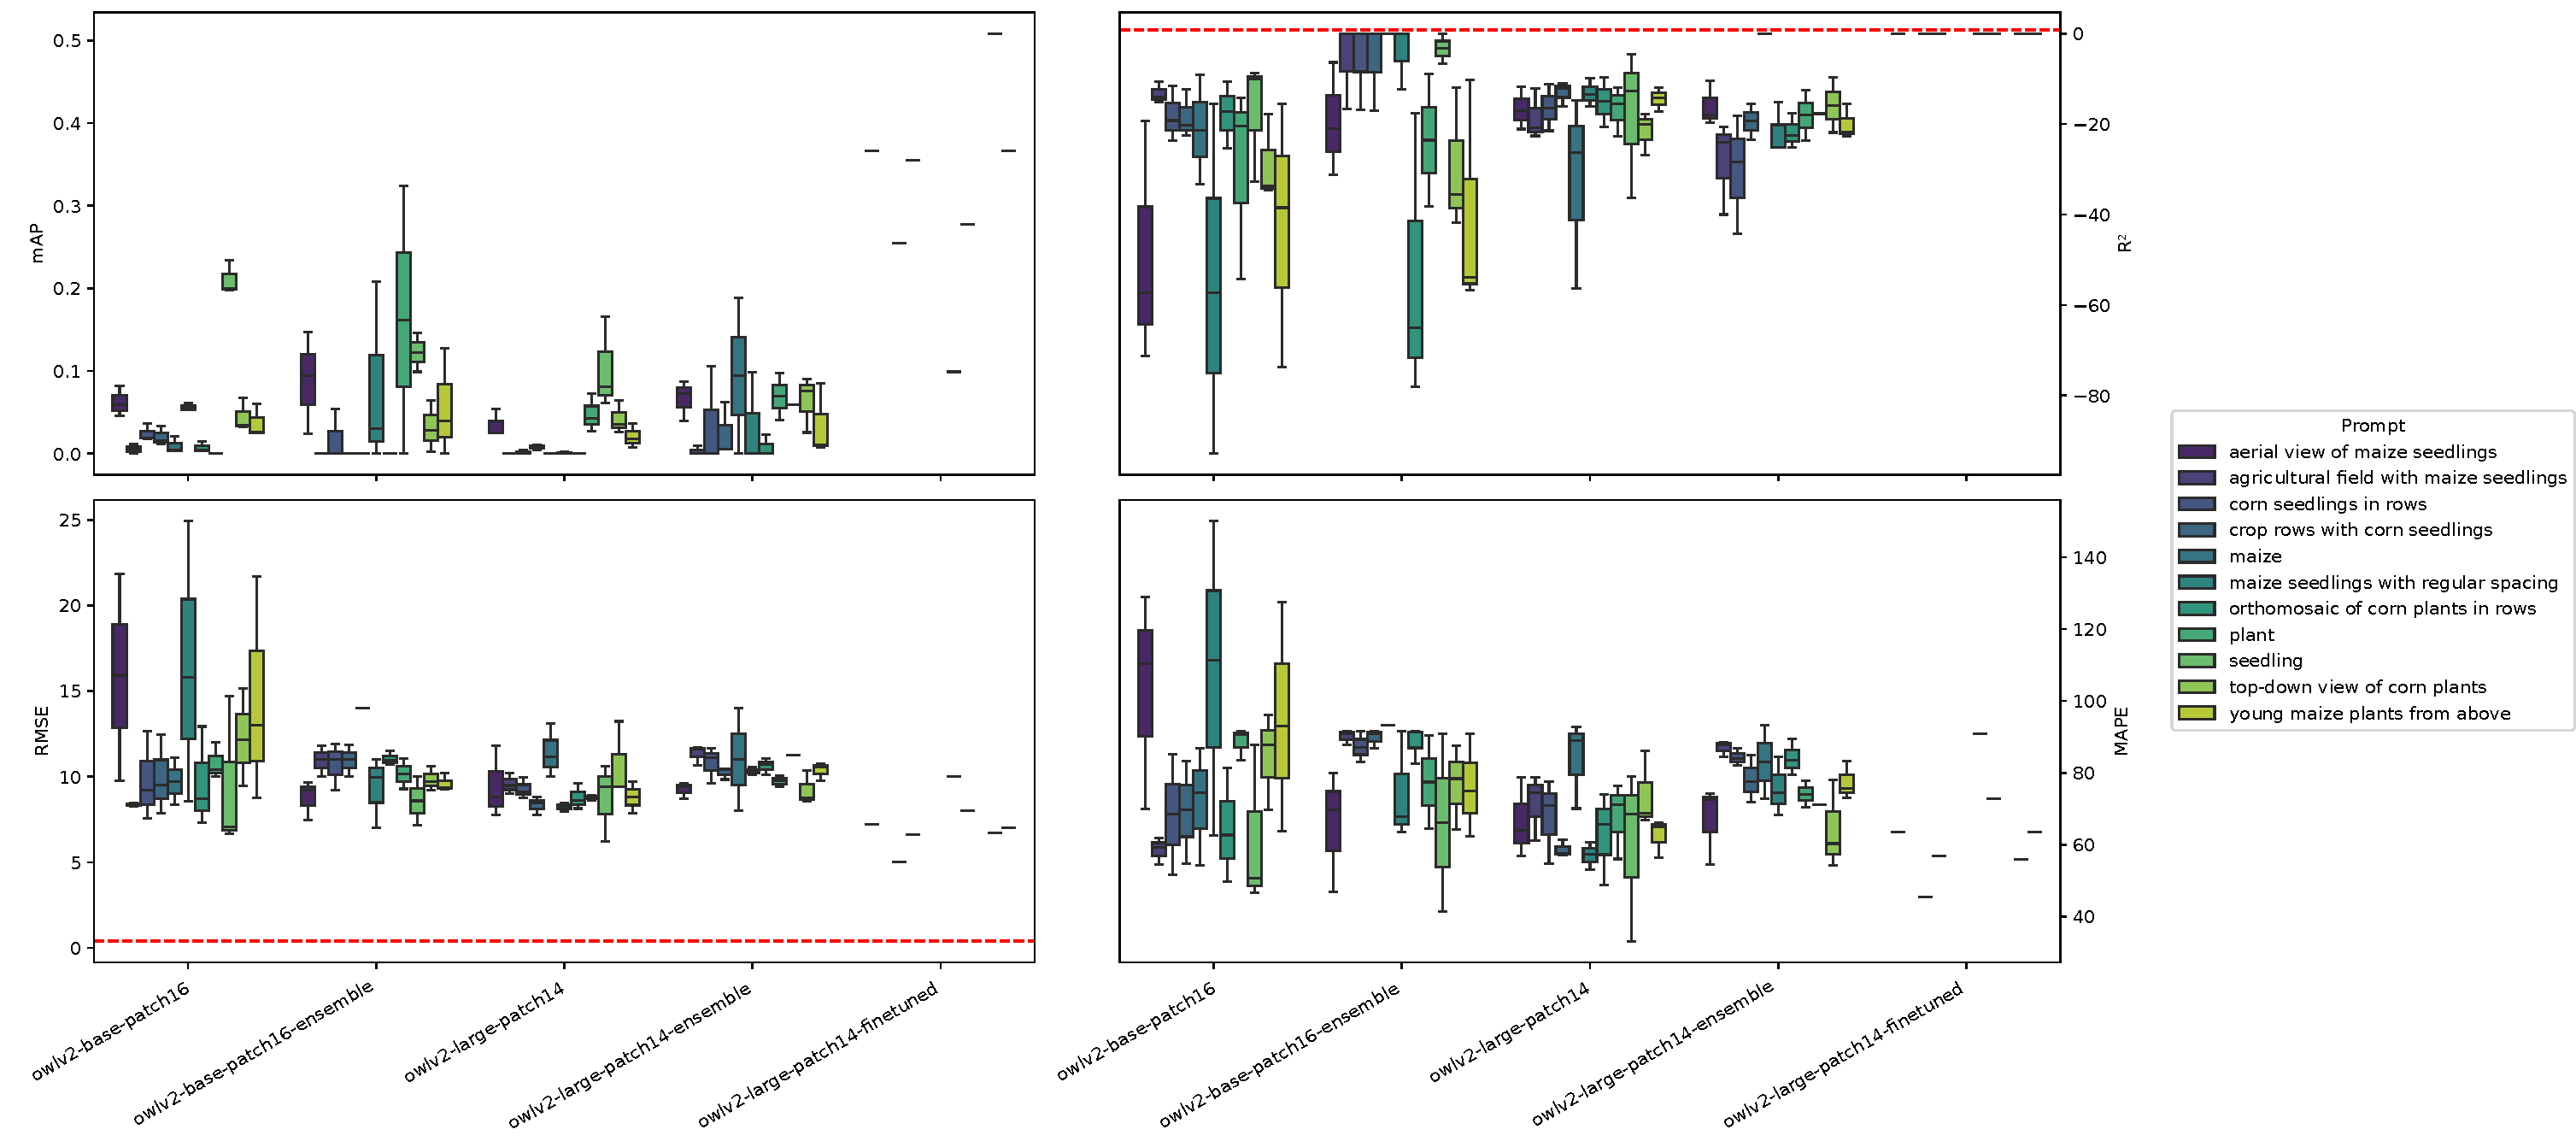
\includegraphics[width=22cm]{Plots/zeroshot.pdf}
  \end{adjustwidth}
  \caption{The figure shows the relationship between the OWLv2 model size, used prompt,
  and model performance.
  The x-axis represents the model settings and the model size.
  Colors represent the different prompts used.
  The four subplots show the $mAP$ (upper left corner), $R^2$ (upper right corner),
  $RMSE$ (lower left corner), and~MAPE (lower right corner) values.
  The red dashed horizontal line in the $R^2$ and the $RMSE$ subplots represents, 
  respectively, the benchmarks of 0.85 and 0.39. 
  }
  \label{fig:zeroshots_vs_performance}
\end{figure}
\end{landscape}

\begin{landscape}
\begin{figure}
  \begin{adjustwidth}{-\extralength}{0cm}
   \centering
  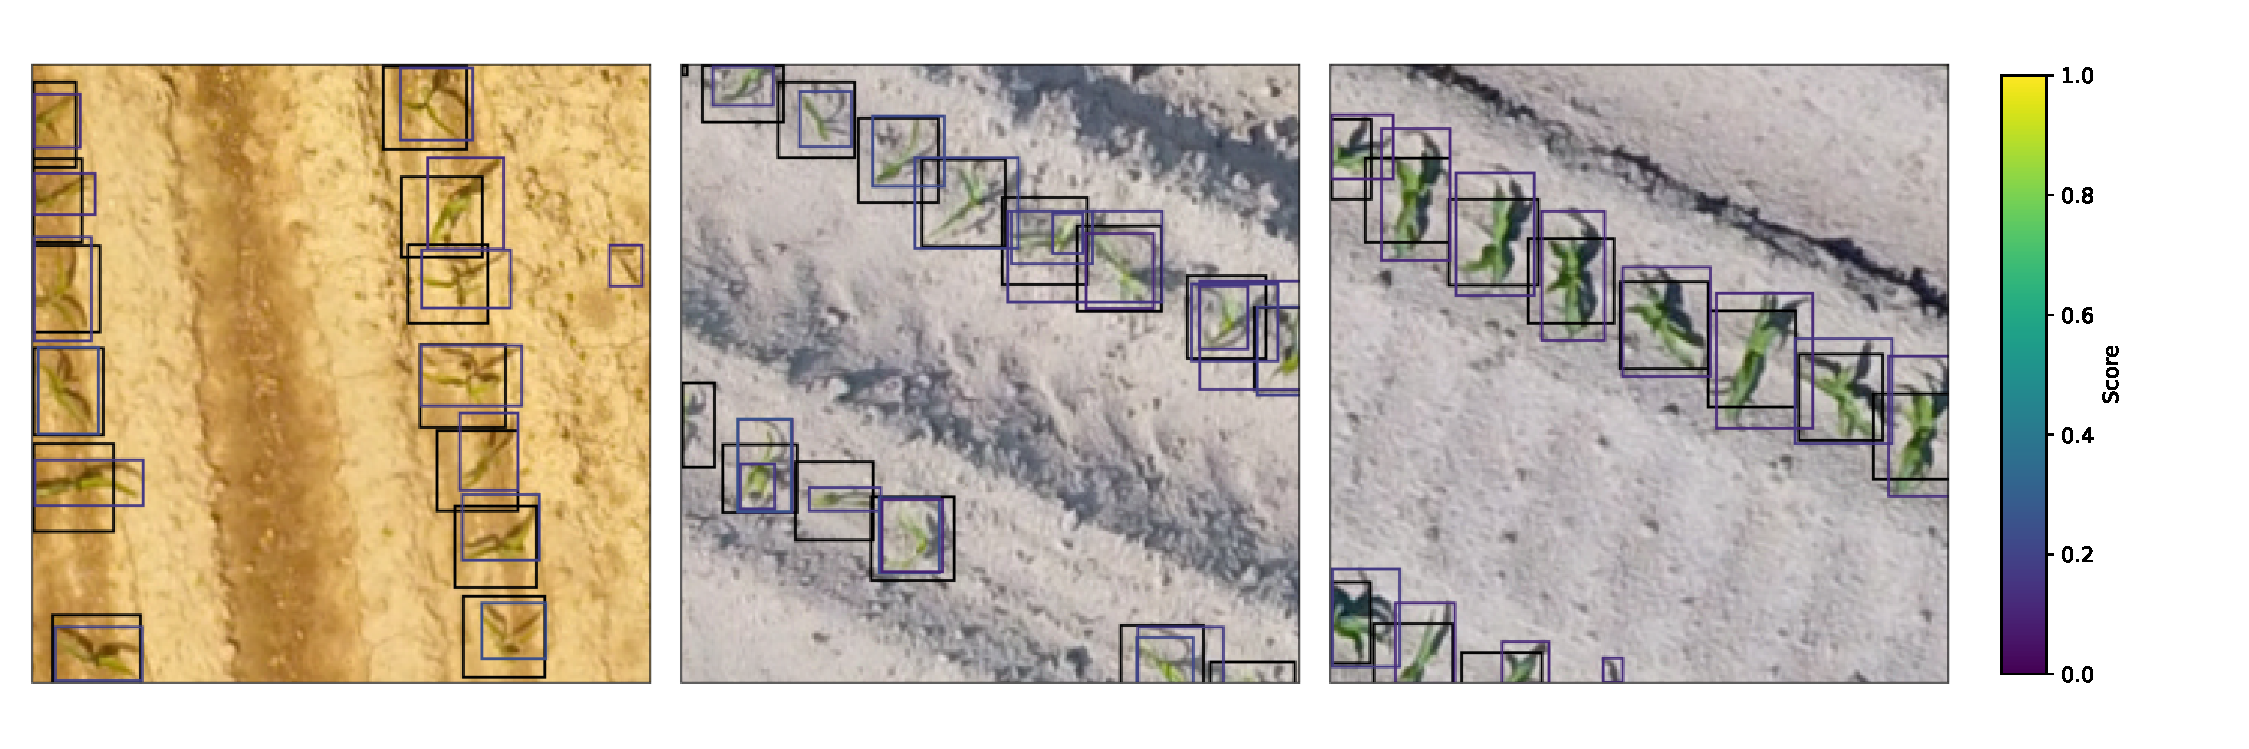
\includegraphics[width=22cm]{Plots/zeroshot_images.pdf}
  \end{adjustwidth}
  \caption{The best predictions with the OWLv2 model.  
  The ID\_1, ID\_2, and ID\_3 datasets, respectively, from the left hand side to the right.
  Prediction with owlv2-base-patch16-ensemble model of the ID\_1 dataset,
  and with owlv2-base-patch16 model on the other two datasets.
  All the predictions are made with the prompt ``seedling''.
  The predicted bounding boxes in the images are the ones before 
  non-maximum suppression and threshold.
  Black bounding boxes are the ground truth annotations, while the bounding boxes 
  in the viridis color scale are the model predictions.}
  \label{fig:annotations_zero-shot}
\end{figure}
\end{landscape}

%%%%%%%%%%%%%%%%%%%%%%%%%%%%%%%%%%%%%%%%%%
\section{Discussion}
\unskip

\subsection{Dataset Source Impact on Object Detection~Performance}
Our experiments clearly demonstrate the critical importance of dataset source 
for successful arable crop seedling detection. None of the tested models, regardless 
of architecture or parameter amount, achieved the benchmark $R^2$ value of 0.85 
when trained on Out-of-Distribution (OOD) datasets. 
Several inherent biases in our datasets likely influenced model performance.
This aligns with previous findings 
by David~et~al.~\cite{davidPlantDetectionCounting2021}  and Andvaag~et~al.~\cite{andvaagCountingCanolaGeneralizable2024}, 
who similarly reported significantly 
lower performance when using training samples from sources different from the inference~dataset.

The domain gap challenge is particularly pronounced in agricultural applications, 
where environmental conditions, lighting, camera parameters, and~plant growth stages 
vary substantially across datasets. The~failure of OOD training highlights that visual 
features learned from one orthomosaic do not generalize well to others without 
significant adaptation. 
As the Goodness-of-Fit ($GoF$) of the models explicating the relationship between dataset size and performance
was always below 0.2, one can argue that the interval of dataset size tested was too narrow
to achieve a good fit or that other variables play an important role in determining model performance.
Both cases are likely to be true, but~also the maximum OOD dataset size that
was tested (1168) was really small in respect to other studies that use training 
datasets of tens of thousand of images to achieve such benchmarks~\cite{badgujarAgriculturalObjectDetection2024}.
This further highlights the importance of collecting in-domain training data, 
as the minimum OOD dataset size and quality to train an object detector to
count arable crops seedling that generalizes to all the real-world cases
is difficult to establish with a limited~dataset. 

Despite the poor performance of OOD dataset-trained models, some of them showed a low $MAPE$ value of less than 20\%,
not enough to consider the models for direct inferencing but rather as an annotation
tool for the ID~dataset.

\subsection{Many-Shot Object Detection: Architecture and Dataset~Requirements}
Our results reveal important relationships between model architecture, count metrics, 
and minimum dataset requirements, consistent with findings from other agricultural computer vision studies. 
Within YOLO-family models, we observed that the lightweight YOLOv5n, YOLOv5s, and~YOLOv8n achieved 
the benchmark with 130, 130, and 110~samples, respectively, well below the  
reported minimum by supposed few-shot studies with the same aim~\cite{karamiAutomaticPlantCounting2020}. 
As already well-known from general computer vision literature~\cite{nguyenEvaluationDeepLearning2020,sunRevisitingUnreasonableEffectiveness2017}, increasing model 
complexity in CNN-based architectures corresponded to increased dataset size~requirements.

Conversely, for~transformer-mixed models like RT-DETR, we observed better performances 
with lower training dataset sizes, with~RT-DETR L achieving 
the benchmark with only 60 samples while the larger RT-DETR X required 100 samples. This superior 
performance of transformer-based models corroborates recent findings~\cite{rekavandiTransformersSmallObject2023,liTransformerObjectDetection2023}, 
who demonstrated that attention mechanisms can achieve better 
performance with limited training data in agricultural contexts. The~empirical models of dataset size 
versus performance showed comparable $GoF$ between RT-DETR and YOLO-family models, except~for YOLOv5n,
which showed a particularly high $GoF$. This suggests that transformer-based models have the same 
predictability to reach the benchmark with the reported dataset size as the CNN-based models, except~for YOLOv5n, which has a higher predictability to reach the benchmark given the same dataset~size.

Overall, transformer-based models may require fewer samples to achieve the same performance as CNN-based models,
potentially due to their ability to capture long-range dependencies and contextual information more effectively, 
as noted in a comprehensive review~\cite{khanSurveyVisionTransformers2023} and demonstrated in agricultural 
applications~\cite{badgujarAgriculturalObjectDetection2024}. A~visible side-effect of the adoption of 
transformer-mixed models is the higher computational cost of the training phase in terms of time and memory, 
which could be a limitation for some applications, consistent with computational trade-offs reported in~\cite{carionEndtoEndObjectDetection2020} but not studied~here.

This creates a practical tradeoff for practitioners: whether to use a simpler CNN-based model like YOLOv5n 
and invest in collecting more annotated images (approximately 130), or~to allocate more computational 
resources for a transformer-mixed model like RT-DETR L that can achieve comparable performance with 
roughly half the amount of labeled data (approximately 60 images). Similar trade-offs have been documented 
in agricultural deployment scenarios by~\cite{torres-sanchez_early_2021} for early-season crop monitoring 
and~\cite{badgujarAgriculturalObjectDetection2024} in their comprehensive review of agricultural object~detection.

The predictability of model performance based on dataset size (as evidenced by $GoF$ values exceeding 0.3 
for successful models) provides practical guidance for practitioners. Our findings on dataset size scaling 
relationships (logarithmic patterns with \mbox{GoF %MDPI: please confirm whether this format should be unified. %Authors: Format confirmed
 > 0.3}) align with broader machine learning scaling laws 
established by~\cite{sunRevisitingUnreasonableEffectiveness2017,hestnessDeepLearningScaling2017}, 
while the agricultural-specific implications mirror domain adaptation challenges documented in~\cite{davidPlantDetectionCounting2021,andvaagCountingCanolaGeneralizable2024}. The~relationship 
between dataset size and performance (modeled using logarithmic, arctangent, or~algebraic root 
functions, depending on best fit) suggests diminishing returns beyond certain thresholds, consistent 
with theoretical frameworks proposed by~\cite{mahmoodHowMuchMore2022}, which can help inform efficient 
resource allocation for annotation efforts in precision agriculture~applications.

\subsection{Dataset Quality~Trade-Offs}
Our investigation into minimum dataset quality requirements revealed that models can tolerate some reduction 
in annotation quality while still maintaining benchmark performance achieved with the
same training dataset size. YOLOv5n, YOLOv5s, and~YOLOv8n achieved 
the benchmark with 85\%, 90\%, and~85\% of the original dataset quality, while RT-DETR X required 
only 65\%. Notably, RT-DETR L failed to maintain benchmark performance with any reduction in annotation quality, 
suggesting different sensitivity to annotation errors, consistent with findings on annotation quality 
effects~\cite{alhazmiEffectsAnnotationQuality2021}.

This difference in quality tolerance between RT-DETR L and RT-DETR X can be explained by considering their 
respective minimum dataset sizes. RT-DETR L was tested with quality reductions on its minimum benchmark-achieving 
dataset size of just 60 samples, while RT-DETR X was tested with 100 samples. With~fewer training examples, 
RT-DETR L becomes more sensitive to the quality of each individual annotation, as~each annotation represents 
a larger proportion of the total learning signal. In~contrast, RT-DETR X, with~its larger training dataset, 
can better compensate for quality reductions by leveraging redundancy across more examples, aligning with 
general principles of dataset robustness~\cite{sunRevisitingUnreasonableEffectiveness2017}.

These findings provide valuable insights for practical applications, as~they suggest that, in some 
cases, it may be more efficient to collect a larger quantity of moderate-quality annotations 
rather than focusing on perfect annotations for a smaller dataset. This also indicates potential 
for semi-automated annotation workflows, where machine assistance in annotation (which may introduce 
some errors) could be acceptable for many applications, supporting approaches documented in 
agricultural computer vision literature~\cite{badgujarAgriculturalObjectDetection2024}.

\subsection{Few-Shot and Zero-Shot Approaches: Current~Limitations}
Despite recent advances in few-shot and zero-shot learning, our experiments reveal significant 
limitations in these approaches for precise maize seedling detection. The~best CD-ViTO few-shot 
model achieved an $RMSE$ of 3.9 with 50 shots (using ViT-B backbone), substantially below the benchmark 
requirement of 0.39. Similarly, zero-shot models like OWLv2 performed poorly, regardless of prompt 
engineering~efforts.

These results contrast with the promising performance reported for few-shot and zero-shot methods 
in general object detection benchmarks~\cite{xuDeViTDecomposingVision2023,mindererScalingOpenVocabularyObject2023}. 
Several factors may explain this gap: 
First, the~domain-specific nature of aerial maize seedling imagery, where subtle 
textural differences and high intra-class variability are prevalent, severely challenges 
models pre-trained on general object detection datasets. As~illustrated in the few-shot 
experiments (Figure \ref{fig:shots_vs_performance}), increasing 
the number of shots leads to nonlinear improvements in metrics such as R² and $mAP$ 
(following an arctan-like trend), yet the error metric ($RMSE$) remain significantly 
above the benchmark. This saturation effect suggests that, even with more than usual maximum tested
prototypes (50 instead of 30), the~models struggle to capture the fine-grained visual cues 
necessary for precise seedling detection. Moreover, the~zero-shot results (Figure 
\ref{fig:zeroshots_vs_performance}) reveal a pronounced sensitivity to prompt phrasing, with~all 
variants, including ensemble and fine-tuned versions of OWLv2, consistently failing 
to approach acceptable error rates. These observations imply that both the inherent 
complexity of the task and the limitations of current few-shot and zero-shot frameworks 
necessitate more domain-specific strategies, as~suggested by recent work on agricultural 
computer vision challenges~\cite{farjon_deep-learning-based_2023}. Addressing these challenges through 
domain-specific adaptations could help narrow the performance gap, potentially making 
few-shot and zero-shot methods more competitive for arable crop seedling detection.
Interestingly, the~few-shot and the zero-shot models were able to detect all the seedlings
without false positives in few cases. It would be interesting to investigate the
possible ways to retain these images and use them to populate the training dataset
for a many-shot~model.

\subsection{Handcrafted Methods in the Deep Learning~Era}
Despite the focus on deep learning approaches, our Handcrafted (HC) object detector 
demonstrated strong performance on the testing datasets ($R^2$ from 0.87 to 0.95). 
However, a~significant limitation was the small proportion of tiles (1.8\% to 7.8\%) 
for which it could provide reliable annotations. This illustrates the classic trade-off 
of rule-based systems: high precision in constrained scenarios but limited generalizability, 
consistent with findings from other agricultural applications using handcrafted methods~\cite{garcia-martinezDigitalCountCorn2020,zhang2020cut}.

These findings suggest that HC methods may still have value in a hybrid approach, where 
they provide high-quality annotations on a subset of data, which can then be used to 
bootstrap deep learning models. Such an approach could be particularly valuable for 
specialized agricultural applications where annotation resources are limited, aligning 
with hybrid approaches documented in crop monitoring studies~\cite{torres-sanchez_early_2021}.

This approach is highly adopted in industry, where the HC method is used to
annotate the training dataset and the deep learning model is used to predict the real-world
cases, but~it introduces a possible bias in the training dataset that could be a limitation
for the model generalization. The~main problem is that the HC1 method relies
on color thresholding that filters the 
objects based on the color of the objects. That could be not the best
way to annotate the training dataset for a deep learning model that could learn
more complex features of the objects, but~also the ones selected by the HC1~method.

\subsection{Implications for Practical~Applications}
Our study has several practical implications for developing arable crop seedling detection systems.
First, collecting in-domain training data is non-negotiable for achieving benchmark performance. 
Finding a way to automatically obtain the training dataset from the same distribution as the intended 
inference target is a key step in developing a robust object detector for arable crop seedling~detection.

The logarithmic relationship between dataset size and performance suggests that initial annotation 
efforts should focus on reaching the minimum viable dataset size (\mbox{60--130 images} depending on architecture), 
after which additional annotations yield diminishing returns. This finding helps organizations optimize 
resource allocation for annotation~efforts.

\textls[-25]{Our results also demonstrate that some reduction in annotation quality is acceptable, with~models maintaining benchmark performance with 65--90\% of the original quality. This suggests that semi-automated annotation workflows could be efficiently implemented for agricultural applications, potentially reducing the time and cost associated with manual annotation.}

Current few-shot and zero-shot methods, while promising, are not yet viable replacements for traditional 
object detection approaches in seedling detection or counting tasks. However, they might still serve 
auxiliary roles in the annotation~pipeline.

Hybrid approaches combining handcrafted methods with deep learning models could provide a practical solution 
for achieving benchmark performance. We observed that OOD many-shot, few-shot, and~zero-shot models are 
occasionally able to produce annotations with sufficient quality for training ID many-shot models. A~promising 
direction for future work would be to develop methods for automatically identifying and leveraging these 
high-quality annotations. Specifically, the~HC2 component of our handcrafted approach could potentially be used 
to filter and validate annotations produced by these models, overcoming the color-thresholding bias introduced 
by HC1 while maintaining the agronomic knowledge encoded in HC2's row-pattern~validation.

\subsection{Future~Work}
In this study, we focused on the minimum dataset requirements for fine-tuning pre-trained models for the 
downstream task of counting arable crop seedlings through object detection. We did not explore the potential 
benefits of using domain-specific backbones. Future work could investigate whether or not dataset size requirements 
could be further reduced by using backbones pre-trained on agricultural imagery, particularly aerial 
orthomosaics of crop fields. Such domain-specific pre-training might allow models to learn more relevant 
features for crop detection tasks, potentially reducing the amount of in-domain data needed for~fine-tuning.

%%%%%%%%%%%%%%%%%%%%%%%%%%%%%%%%%%%%%%%%%%
\section{Conclusions}

This study demonstrates that successful maize seedling detection requires in-domain 
training data, with~out-of-distribution training requiring unreasonable dataset size to 
achieve benchmark performance across all tested models. 
We established minimum dataset requirements for several 
architectures, finding that lightweight YOLO models achieve benchmark performance 
with 110--130 samples, while certain transformer-mixed models like RT-DETR require as 
few as 60 samples. Models showed varying tolerance for reduced annotation quality, 
with some maintaining performance with only 65--90\% of original annotation~quality.

Despite advances in machine learning, neither few-shot nor zero-shot approaches currently 
meet precision requirements for arable crop seedling detection. Our handcrafted 
algorithm achieved excellent performance within its constraints, suggesting potential 
value in hybrid approaches combining rule-based methods with deep learning. These 
findings provide practical guidance for developing maize seedling detection 
systems, and~possible ways to overcome the limitations of the current deep learning
models for this~application.
 
% This section is not mandatory, but can be added to the manuscript if the discussion 
% is unusually long or complex.

%%%%%%%%%%%%%%%%%%%%%%%%%%%%%%%%%%%%%%%%%%
% \section{Patents}

% This section is not mandatory, but may be added if there are patents resulting from 
% the work reported in this manuscript.

%%%%%%%%%%%%%%%%%%%%%%%%%%%%%%%%%%%%%%%%%%
\vspace{6pt} 

%%%%%%%%%%%%%%%%%%%%%%%%%%%%%%%%%%%%%%%%%%
%% optional
%\supplementary{The following supporting information can be downloaded at:  \linksupplementary{s1}, Figure S1: title; Table S1: title; Video S1: title.}

% Only for journal Methods and Protocols:
% If you wish to submit a video article, please do so with any other supplementary material.
% \supplementary{The following supporting information can be downloaded at: \linksupplementary{s1}, Figure S1: title; Table S1: title; Video S1: title. A supporting video article is available at doi: link.}

% Only used for preprtints:
% \supplementary{The following supporting information can be downloaded at the website of this paper posted on \href{https://www.preprints.org/}{Preprints.org}.}

% Only for journal Hardware:
% If you wish to submit a video article, please do so with any other supplementary material.
% \supplementary{The following supporting information can be downloaded at: \linksupplementary{s1}, Figure S1: title; Table S1: title; Video S1: title.\vspace{6pt}\\
%\begin{tabularx}{\textwidth}{lll}
%\toprule
%\textbf{Name} & \textbf{Type} & \textbf{Description} \\
%\midrule
%S1 & Python script (.py) & Script of python source code used in XX \\
%S2 & Text (.txt) & Script of modelling code used to make Figure X \\
%S3 & Text (.txt) & Raw data from experiment X \\
%S4 & Video (.mp4) & Video demonstrating the hardware in use \\
%... & ... & ... \\
%\bottomrule
%\end{tabularx}
%}

%%%%%%%%%%%%%%%%%%%%%%%%%%%%%%%%%%%%%%%%%%
\authorcontributions{Conceptualization, S.B. and E.B.-M.; methodology, S.B. and E.B.-M.; \mbox{software, S.B.}; validation, S.B.; formal analysis, S.B.; investigation, S.B.; resources, S.B. and \mbox{E.B.-M.}; data curation, S.B.; writing---original draft preparation, S.B.; writing---review and editing, E.B.-M.; visualization, S.B.; supervision, E.B.-M.; project administration, E.B.-M.; funding acquisition, S.B. and E.B.-M. All authors have read and agreed to the published version of the manuscript.}

\funding{This research was conducted as part of a PhD program supported by SAGEA centro di saggio~s.r.l.}

% \institutionalreview{In this section, you should add the Institutional Review Board 
% Statement and approval number, if relevant to your study. You might choose to exclude 
% this statement if the study did not require ethical approval. Please note that the 
% Editorial Office might ask you for further information. Please add “The study was 
% conducted in accordance with the Declaration of Helsinki, and approved by the Institutional 
% Review Board (or Ethics Committee) of NAME OF INSTITUTE (protocol code XXX and date of 
% approval).” for studies involving humans. OR “The animal study protocol was approved by 
% the Institutional Review Board (or Ethics Committee) of NAME OF INSTITUTE (protocol 
% code XXX and date of approval).” for studies involving animals. OR “Ethical review 
% and approval were waived for this study due to REASON (please provide a detailed 
% justification).” OR “Not applicable” for studies not involving humans or animals.}

% \informedconsent{Any research article describing a study involving humans should 
% contain this statement. Please add ``Informed consent was obtained from all subjects 
% involved in the study.'' OR ``Patient consent was waived due to REASON (please provide 
% a detailed justification).'' OR ``Not applicable'' for studies not involving humans. 
% You might also choose to exclude this statement if the study did not involve humans.

% Written informed consent for publication must be obtained from participating patients 
% who can be identified (including by the patients themselves). Please state ``Written 
% informed consent has been obtained from the patient(s) to publish this paper'' if 
% applicable.}

% \dataavailability{We encourage all authors of articles published in MDPI journals 
% to share their research data. In this section, please provide details regarding where 
% data supporting reported results can be found, including links to publicly archived 
% datasets analyzed or generated during the study. Where no new data were created, or 
% where data is unavailable due to privacy or ethical restrictions, a statement is 
% still required. Suggested Data Availability Statements are available in section 
% ``MDPI Research Data Policies'' at \url{https://www.mdpi.com/ethics}.}

\dataavailability{The code for the handcrafted methods used 
in this study is available at %MDPI: Please provide the date you accessed the URL in the following format: “URL (accessed on Day Month Year)”.
 \url{https://gist.github.com/SamueleBumbaca/4a227bbe7b78d6be3424899c16c60bb4} (accessed on 20 June 2025). %MDPI: we found that this url is not accessible. Please check and revise!! %Authors: We decided to use a Gist instead of a GitHub repository, as it is more suitable for sharing small code snippets. The link is now accessible.
% also we decided to not republish the code for the deep learning methods, as it is not the main focus of this study and it is already available in the original papers.
The datasets created during this study (ID datasets) are available at the Zenodo 
repository \url{ https://doi.org/10.5281/zenodo.15235602} (accessed on 20 June 2025)%MDPI: please provide the date you accessed the URL in the following format: “URL (accessed on Day Month Year).
. The~other datasets used are available from their 
cited sources.}

% Only for journal Drones
%\durcstatement{Current research is limited to the [please insert a specific academic field, e.g.,~XXX], which is beneficial [share benefits and/or primary use] and does not pose a threat to public health or national security. Authors acknowledge the dual-use potential of the research involving xxx and confirm that all necessary precautions have been taken to prevent potential misuse. As an ethical responsibility, authors strictly adhere to relevant national and international laws about DURC. Authors advocate for responsible deployment, ethical considerations, regulatory compliance, and transparent reporting to mitigate misuse risks and foster beneficial outcomes.}

% Only for journal Nursing Reports
%\publicinvolvement{Please describe how the public (patients, consumers, carers) were involved in the research. Consider reporting against the GRIPP2 (Guidance for Reporting Involvement of Patients and the Public) checklist. If the public were not involved in any aspect of the research add: ``No public involvement in any aspect of this research''.}
%
%% Only for journal Nursing Reports
%\guidelinesstandards{Please add a statement indicating which reporting guideline was used when drafting the report. For example, ``This manuscript was drafted against the XXX (the full name of reporting guidelines and citation) for XXX (type of research) research''. A complete list of reporting guidelines can be accessed via the equator network: \url{https://www.equator-network.org/}.}
%
%% Only for journal Nursing Reports
%\useofartificialintelligence{Please describe in detail any and all uses of artificial intelligence (AI) or AI-assisted tools used in the preparation of the manuscript. This may include, but is not limited to, language translation, language editing and grammar, or generating text. Alternatively, please state that “AI or AI-assisted tools were not used in drafting any aspect of this manuscript”.}

%\acknowledgments{}
% In this section you can acknowledge any support given which is 
% not covered by the author contribution or funding sections. This may include administrative 
% and technical support, or donations in kind (e.g., materials used for experiments).}

\conflictsofinterest{The authors declare 
no conflicts of interest. The funders had no role in the 
design of the study; in the collection, analyses, or~interpretation of data; in 
the writing of the manuscript; or in the decision to publish the~results.} 

%%%%%%%%%%%%%%%%%%%%%%%%%%%%%%%%%%%%%%%%%%
%% Optional

%% Only for journal Encyclopedia
%\entrylink{The Link to this entry published on the encyclopedia platform.}

%\pagebreak

\section*{Abbreviations}
The following abbreviations are used in this manuscript:

\noindent 
\begin{tabular}{@{}ll}
$R^2$ & Coefficient of determination\\
$RMSE$ & Root Mean Squared Error\\
$MAPE$ & Mean Absolute Percentage Error\\
$mAP$ & Mean Average Precision\\
HC & Handcrafted\\
ID & In-Distribution\\
OOD & Out-of-Distribution\\
CNN & Convolutional Neural Network\\
ViT & Vision Transformer\\
YOLO & You Only Look Once\\
RT-DETR & Real-Time Detection Transformer\\
GoF & Goodness of Fit\\
\end{tabular}

%%%%%%%%%%%%%%%%%%%%%%%%%%%%%%%%%%%%%%%%%%
%% Optional
\appendixtitles{no} % Leave argument "no" if all appendix headings stay EMPTY (then no dot is printed after "Appendix A"). If~the appendix sections contain a heading then change the argument to "yes".
% Appendix section
\section[\appendixname~\thesection]{}
\subsection[\appendixname~\thesubsection]{}
\vspace{-2pt}
\begin{algorithm}[H]
  \caption{H1}
  \label{alg:H1}
  \begin{algorithmic}[1]
  \Require $tiles$ \Comment{Orthomosaic tiles}
  \Require $col\_range$ \Comment{Color space thresholds}
  \Require $leaf\_area\_range$ \Comment{Leaf area range in pixels}
  \Ensure $plants$ \Comment{List of polygons}
  
  \Function{connected\_components}{$binary\_image$} \cite{wuOptimizingConnectedComponent2005} 
      \State \Return $regions$
  \EndFunction
  
  \For{$tile$ in $tiles$}
    \State $mask \gets \{p \in tile \mid color(p) \in col\_range\}$
    \State $regions \gets connected\_components(mask)$
    \State $plants \gets \{region \mid region \in regions \land region.area \in leaf\_area\_range\}$
  \EndFor
  \State \Return $plants$
\end{algorithmic}
\end{algorithm}

  
  \vspace{-6pt}

\begin{algorithm}[H]
\caption{H2}
\label{alg:H2}
\small
\begin{algorithmic}[1]
\Require $observations$ \Comment{(List of centroids, RanSaC models)}
\Require $intra-row\_dist$ \Comment{Minimum distance between plants}
\Require $inter-row\_dist$ \Comment{Minimum distance between rows}
\Require $mean\_slope$ \Comment{Mean slope of the rows in respect meridian}
\Ensure $objects$ \Comment{List of centroids or polygons}
\Function{region\_centroids}{$regions$} \Comment{Get the centroids of the regions}
  \State \Return $centroids$
\EndFunction
\Function{agglomerate\_regions}{$regions, min\_dist$} \Comment{Agglomerate regions}
  \State $centroids \gets \{region.centroid \mid region \in regions\}$
  \State \textls[-30]{$clusters \gets \text{HierarchicalClustering}(centroids, threshold=min\_dist, metric=\text{euclidean})$}
  \State $clust\_cen \gets \{\text{mean}(centroids_i) \mid \text{for each cluster } i \in clusters\}$
  \State \Return $clust\_cen$
\EndFunction
\Function{extract\_ransac\_line}{$points,  min\_dist$} \cite{fischlerRandomSampleConsensus1987}
  \State \Return $best\_inliers, best\_model$
\EndFunction
\Function{process\_tiles}{$intra-row\_dist$}

  \State $observations \gets \{\}$
  \State $plants \gets \Call{HC1}{tiles}$
  \For{$tile$ in $tiles$}
    \State $regions \gets plants[tile]$
    \State $centroids \gets \Call{region\_centroids}{regions}$
    \State $clust\_cen \gets \Call{agglomerate\_regions}{regions, intra-row\_dist}$
    \State $inlier\_points, model \gets \Call{extract\_ransac\_line}{clust\_cen, intra-row\_dist}$
    \State $line\_length \gets \Call{get\_line\_length}{model}$
    \State $expected\_number\_of\_plants \gets \frac{line\_length}{intra\_row\_dist}$
    \If {$inlier\_points \equiv expected\_number\_of\_plants}$
      \State $observations[tile] \gets (clust\_cen,inlier\_points,model)$
    \EndIf
  \EndFor
  \State \Return $observations$
\EndFunction
    
    \algstore{myalg}
\end{algorithmic}
\end{algorithm}
 
 
 
 
\begin{algorithm}[H]
\addtocounter{algorithm}{-1}
\caption{\textit{Cont.}}
\label{alg:H2}
\small
\begin{algorithmic}[1]
 
\algrestore{myalg}
\Function{Filter\_observations\_by\_slope}{$observations$}
  \State $filtered\_observations \gets \{\}$
  \For{$tile \in observations$}
    \State $slope \gets observations[tile][\text{'model'}]$
    \If{$model.slope \approx mean\_slope$}
      \State $filtered\_observations[tile] \gets observations[tile]$
    \EndIf
  \EndFor
  \State \Return $filtered\_observations$
\EndFunction
\Function{process\_observations}{$observations,inter-row\_dist,intra-row\_dist$}
  \State $objects \gets \{\}$
  \For{$tile \in observations$}
    \State $tile\_centers \gets observations[tile][\text{'clust\_cen'}]$
    \State $first\_row\_centers \gets observations[tile][\text{'inlier\_points'}]$
    \State $first\_row\_model \gets observations[tile][\text{'model'}]$
    \State $centers \gets \{p \mid p \in tile\_centers \land p \notin first\_row\_centers\}$
    \State $second\_row\_centers, second\_row\_model \gets \Call{extract\_ransac\_line}{centers, intra-row\_dist}$
    \State $line\_length \gets \Call{get\_line\_length}{second\_row\_model}$
    \State $expected\_number\_of\_plants \gets \frac{line\_length}{intra\_row\_dist}$
    \If {$second\_row\_model.slope \approx first\_row\_model.slope$}
      \If {$abs(second\_row\_model.intercept - first\_row\_model.intercept) \approx inter-row\_dist$}
        \If {$second\_row\_centers \equiv expected\_number\_of\_plants}$
          \State $objects[tile] \gets (first\_row\_centers, second\_row\_centers)$
        \EndIf
      \EndIf
    \EndIf
  \EndFor
  \State \Return $objects$
\EndFunction
\Function{main}{}
  \State $observations \gets \Call{process\_tiles}{intra-row\_dist}$
  \State $MEAN\_SLOPE \gets \Call{mean}{observations[\text{'model'}]}$
  \State $observations \gets \Call{Filter\_observations\_by\_slope}{observations,MEAN\_SLOPE}$
  \State $objects \gets \Call{process\_observations}{observations,inter-row\_dist}$
  \State \Return $objects$
\EndFunction
\end{algorithmic}
\end{algorithm}


\subsection[\appendixname~\thesubsection]{}
The following are the list of prompts used for the zero-shot~models:
\begin{itemize}
    \item ``maize''
    \item ``seedling''
    \item ``plant''
    \item ``aerial view of maize seedlings''
    \item ``corn seedlings in rows''
    \item ``young maize plants from above''
    \item ``crop rows with corn seedlings''
    \item ``maize seedlings with regular spacing''
    \item ``top-down view of corn plants''
    \item ``agricultural field with maize seedlings''
    \item ``orthomosaic of corn plants in rows''
\end{itemize}

\reftitle{References}

\begin{thebibliography}{999}

\bibitem[Blandino et~al.(2016)Blandino, Testa, Quaglini, and
Reyneri]{blandinoeffetto2016}
Blandino, M.; Testa, G.; Quaglini, L.; Reyneri, A.
\newblock {\em Effetto Della Densità Colturale e Dell'Applicazione di
Fungicidi Sulla Produzione e la Qualità del Mais da Granella e da
Trinciato}; ITA: Rome, Italy, 
2016.


\bibitem[Lu et~al.(2023)Lu, Ye, Wang, and Yu]{10287390}
Lu, D.; Ye, J.; Wang, Y.; Yu, Z.
\newblock Plant Detection and Counting: Enhancing Precision Agriculture in UAV
and General Scenes.
\newblock {\em IEEE Access} {\bf 2023}, {\em 11},~116196--116205. [\href{http://doi.org/10.1109/ACCESS.2023.3325747}{CrossRef}]

\bibitem[Saatkamp et~al.(2019)Saatkamp, Cochrane, Commander, Guja,
Jimenez-Alfaro, Larson, Nicotra, Poschlod, Silveira, Cross, Dalziell, Dickie,
Erickson, Fidelis, Fuchs, Golos, Hope, Lewandrowski, Merritt, Miller, Miller,
Offord, Ooi, Satyanti, Sommerville, Tangney, Tomlinson, Turner, and
Walck]{Saatkamp2019AResearchAF}
Saatkamp, A.; Cochrane, A.; Commander, L.; Guja, L.; Jimenez-Alfaro, B.;
Larson, J.; Nicotra, A.; Poschlod, P.; Silveira, F.A.O.; Cross, A.;  et~al.
\newblock A research agenda for seed-trait functional ecology.
\newblock {\em New Phytol.} {\bf 2019}, {\em 221},~1764--1775. [\href{http://dx.doi.org/10.1111/nph.15502}{CrossRef}] [\href{http://www.ncbi.nlm.nih.gov/pubmed/30269352}{PubMed}]

\bibitem[De~Petris et~al.(2021)De~Petris, Sarvia, Gullino, Tarantino, and
Borgogno-Mondino]{rs13051030}
De~Petris, S.; Sarvia, F.; Gullino, M.; Tarantino, E.; Borgogno-Mondino, E.
\newblock Sentinel-1 Polarimetry to Map Apple Orchard Damage after a Storm.
\newblock {\em Remote Sens.} {\bf 2021}, {\em 13}, 1030. [\href{http://dx.doi.org/10.3390/rs13051030}{CrossRef}]

\bibitem[PP1(2024)]{PP13332024}
{{{\textsc{PP}}}} 1/333 (1) {{Adoption}} of Digital Technology for Data
Generation for the Efficacy Evaluation of Plant Protection Products.
\newblock {\em EPPO Bull.} {\bf 2025}, {\em 55}, 14--19. [\href{http://dx.doi.org/10.1111/epp.13037}{CrossRef}]

\bibitem[Zou et~al.(2020)Zou, Lu, Li, Liu, and
Cao]{zouMaizeTasselsDetection2020}
Zou, H.; Lu, H.; Li, Y.; Liu, L.; Cao, Z.
\newblock Maize Tassels Detection: A Benchmark of the State of the Art.
\newblock {\em Plant Methods} {\bf 2020}, {\em 16},~108. [\href{http://dx.doi.org/10.1186/s13007-020-00651-z}{CrossRef}]

\bibitem[Lin et~al.(2015)Lin, Maire, Belongie, Bourdev, Girshick, Hays, Perona,
Ramanan, Zitnick, and Doll{\'a}r]{linMicrosoftCOCOCommon2015}
Lin, T.Y.; Maire, M.; Belongie, S.; Bourdev, L.; Girshick, R.; Hays, J.;
Perona, P.; Ramanan, D.; Zitnick, C.L.; Doll{\'a}r, P.
\newblock Microsoft {{COCO}}: {{Common Objects}} in {{Context}}. {\em arXiv} {\bf 2015}, arXiv:1405.0312.
\newblock [\href{https://doi.org/10.48550/arXiv.1405.0312}{CrossRef}]

\bibitem[Kraus(2011)]{krausPhotogrammetryGeometryImages2011}
Kraus, K.
\newblock {\em Photogrammetry: {{Geometry}} from {{Images}} and {{Laser
Scans}}}; De Gruyter: Berlin, Germany, 2011. [\href{http://dx.doi.org/10.1515/9783110892871}{CrossRef}]

\bibitem[Pugh et~al.(2021)Pugh, Thorp, Gonzalez, Elshikha, and
Pauli]{pugh_comparison_2021}
Pugh, N.A.; Thorp, K.R.; Gonzalez, E.M.; Elshikha, D.E.M.; Pauli, D.
\newblock Comparison of image georeferencing strategies for agricultural
applications of small unoccupied aircraft systems.
\newblock {\em  Plant Phenome J.} {\bf 2021}, {\em 4},~e20026. [\href{http://dx.doi.org/10.1002/ppj2.20026}{CrossRef}]

\bibitem[Dhonju et~al.(2023)Dhonju, Walsh, and Bhattarai]{dhonju_web_2023}
Dhonju, H.K.; Walsh, K.B.; Bhattarai, T.
\newblock Web {Mapping} for {Farm} {Management} {Information} {Systems}: {A}
{Review} and {Australian} {Orchard} {Case} {Study}.
\newblock {\em Agronomy} {\bf 2023}, {\em 13},~2563. [\href{http://dx.doi.org/10.3390/agronomy13102563}{CrossRef}]

\bibitem[Habib et~al.(2016)Habib, Han, Xiong, He, Zhang, and
Crawford]{habib_automated_2016}
Habib, A.; Han, Y.; Xiong, W.; He, F.; Zhang, Z.; Crawford, M.
\newblock Automated {Ortho}-{Rectification} of {UAV}-{Based} {Hyperspectral}
{Data} over an {Agricultural} {Field} {Using} {Frame} {RGB} {Imagery}.
\newblock {\em Remote Sens.} {\bf 2016}, {\em 8},~796. [\href{http://dx.doi.org/10.3390/rs8100796}{CrossRef}]

\bibitem[De~Petris et~al.(2020)De~Petris, Sarvia, and
Borgogno-Mondino]{de_petris_rpas-based_2020}
De~Petris, S.; Sarvia, F.; Borgogno-Mondino, E.
\newblock {RPAS}-based photogrammetry to support tree stability assessment:
{Longing} for precision arboriculture.
\newblock {\em Urban For. Urban Green.} {\bf 2020}, {\em 55},~126862. [\href{http://dx.doi.org/10.1016/j.ufug.2020.126862}{CrossRef}]

\bibitem[Zhang et~al.(2022)Zhang, Barrett, Baros, Neville, Talasila, and
Sinclair]{zhang_georeferencing_2022}
Zhang, S.; Barrett, H.A.; Baros, S.V.; Neville, P.R.H.; Talasila, S.; Sinclair,
L.L.
\newblock Georeferencing {Accuracy} {Assessment} of {Historical} {Aerial}
{Photos} {Using} a {Custom}-{Built} {Online} {Georeferencing} {Tool}.
\newblock {\em ISPRS Int. J. Geo-Inf.} {\bf 2022}, {\em
11},~582. [\href{http://dx.doi.org/10.3390/ijgi11120582}{CrossRef}]

\bibitem[Farjon et~al.(2023)Farjon, Huijun, and
Edan]{farjon_deep-learning-based_2023}
Farjon, G.; Huijun, L.; Edan, Y.
\newblock Deep-learning-based counting methods, datasets, and applications in
agriculture: A review.
\newblock {\em Precis. Agric.} {\bf 2023}, {\em 24},~1683--1711. [\href{http://dx.doi.org/10.1007/s11119-023-10034-8}{CrossRef}]

\bibitem[Meier et~al.(2009)Meier, Bleiholder, Buhr, Feller, Hack, He{\ss},
Lancashire, Schnock, Stau{\ss}, van~den Boom, Weber, and
Zwerger]{meierBBCHSystemCoding2009}
Meier, U.; Bleiholder, H.; Buhr, L.; Feller, C.; Hack, H.; He{\ss}, M.;
Lancashire, P.D.; Schnock, U.; Stau{\ss}, R.; van~den Boom, T.;  et~al.
\newblock The {{BBCH}} System to Coding the Phenological Growth Stages of
Plants-History and Publications.
\newblock {\em J. F{\"u}r Kult.} {\bf 2009}, {\em 61},~41--52. [\href{http://dx.doi.org/10.5073/JfK.2009.02.01}{CrossRef}]

\bibitem[David et~al.(2021)David, Daubige, Joudelat, Burger, Comar, {de Solan},
and Baret]{davidPlantDetectionCounting2021}
David, E.; Daubige, G.; Joudelat, F.; Burger, P.; Comar, A.; {de Solan}, B.;
Baret, F.
\newblock Plant Detection and Counting from High-Resolution {{RGB}} Images
Acquired from {{UAVs}}: Comparison between Deep-Learning and Handcrafted
Methods with Application to Maize, Sugar Beet, and Sunflower. {\em bioRxiv} {\bf2021}. [\href{http://dx.doi.org/10.1101/2021.04.27.441631}{CrossRef}]

\bibitem[Liu et~al.(2022)Liu, Zhou, Wang, Costa, Kaeppler, and
Zhang]{liuIntegrateNetDeepLearning2022}
Liu, W.; Zhou, J.; Wang, B.; Costa, M.; Kaeppler, S.M.; Zhang, Z.
\newblock {{IntegrateNet}}: {{A Deep Learning Network}} for {{Maize Stand
Counting From UAV Imagery}} by {{Integrating Density}} and {{Local Count
Maps}}.
\newblock {\em IEEE Geosci. Remote Sens. Lett.} {\bf 2022}, {\em
19}, 6512605. [\href{http://dx.doi.org/10.1109/LGRS.2022.3186544}{CrossRef}]

\bibitem[Mai({\natexlab{a}})]{Maize_seedingDatasetOverview}
Maize\_seeding {{Dataset}} {$>$} {{Overview}}.
\newblock Available online: \url{https://universe.roboflow.com/objectdetection-hytat/maize\_seeding} (accessed on 
20 June 2025).


\bibitem[Mai({\natexlab{b}})]{MaizeseedlingdetectionDatasetOverview}
Maize-Seedling-Detection {{Dataset}} {$>$} {{Overview}}.
\newblock
Available online: \url{https://universe.roboflow.com/fyxdds-icloud-com/maize-seedling-detection} (accessed on 20 June 2025).

\bibitem[{FAO}(2024)]{fao2024}
{FAO}.
\newblock {\em Agricultural Production Statistics 2010--2023}; Volume Analytical Briefs; FAOSTAT:
Rome, Italy, 2024.

\bibitem[Torres-Sánchez et~al.(2021)Torres-Sánchez, Mesas-Carrascosa,
Jiménez-Brenes, de~Castro, and López-Granados]{torres-sanchez_early_2021}
Torres-Sánchez, J.; Mesas-Carrascosa, F.J.; Jiménez-Brenes, F.M.; de~Castro,
A.I.; López-Granados, F.
\newblock Early {Detection} of {Broad}-{Leaved} and {Grass} {Weeds} in {Wide}
{Row} {Crops} {Using} {Artificial} {Neural} {Networks} and {UAV} {Imagery}.
\newblock {\em Agronomy} {\bf 2021}, {\em 11},~749. [\href{http://dx.doi.org/10.3390/agronomy11040749}{CrossRef}]

\bibitem[Zhang et~al.(2020)Zhang, Cao, Peng, Liu, Sun, Zhang, and
Li]{zhang2020cut}
Zhang, Z.; Cao, R.; Peng, C.; Liu, R.; Sun, Y.; Zhang, M.; Li, H.
\newblock Cut-edge detection method for rice harvesting based on machine
vision.
\newblock {\em Agronomy} {\bf 2020}, {\em 10},~590. [\href{http://dx.doi.org/10.3390/agronomy10040590}{CrossRef}]

\bibitem[{Garc{\'i}a-Mart{\'i}nez} et~al.(2020){Garc{\'i}a-Mart{\'i}nez},
{Flores-Magdaleno}, {Khalil-Gardezi}, {Ascencio-Hern{\'a}ndez},
{Tijerina-Ch{\'a}vez}, {V{\'a}zquez-Pe{\~n}a}, and
{Mancilla-Villa}]{garcia-martinezDigitalCountCorn2020}
{Garc{\'i}a-Mart{\'i}nez}, H.; {Flores-Magdaleno}, H.; {Khalil-Gardezi}, A.;
{Ascencio-Hern{\'a}ndez}, R.; {Tijerina-Ch{\'a}vez}, L.;
{V{\'a}zquez-Pe{\~n}a}, M.A.; {Mancilla-Villa}, O.R.
\newblock Digital {{Count}} of {{Corn Plants Using Images Taken}} by {{Unmanned
Aerial Vehicles}} and {{Cross Correlation}} of {{Templates}}.
\newblock {\em Agronomy} {\bf 2020}, {\em 10},~469. [\href{http://dx.doi.org/10.3390/agronomy10040469}{CrossRef}]

\bibitem[LeCun et~al.(2015)LeCun, Bengio, and Hinton]{lecunDeepLearning2015}
LeCun, Y.; Bengio, Y.; Hinton, G.
\newblock Deep Learning.
\newblock {\em Nature} {\bf 2015}, {\em 521},~436--444. [\href{http://dx.doi.org/10.1038/nature14539}{CrossRef}]

\bibitem[Fas()]{FasterRCNNRealTime}
Faster {{R-CNN}}: {{Towards Real-Time Object Detection}} with {{Region Proposal
Networks}}{\textbar}{{IEEE Journals}} \& {{Magazine}}{\textbar}{{IEEE
Xplore}}.
\newblock Available online: \url{https://ieeexplore-ieee-org.bibliopass.unito.it/document/7485869} (accessed on 20 June 2025).
\newpage
\bibitem[You()]{YouOnlyLook}
You {{Only Look Once}}: {{Unified}}, {{Real-Time Object Detection}}{\textbar}{{IEEE Conference Publication}}{\textbar}{{IEEE Xplore}}.
\newblock Available online: \url{https://ieeexplore-ieee-org.bibliopass.unito.it/document/7780460} (accessed on 20 June 2025).

\bibitem[Vaswani et~al.(2017)Vaswani, Shazeer, Parmar, Uszkoreit, Jones, Gomez,
Kaiser, and Polosukhin]{vaswaniAttentionAllYou2017}
Vaswani, A.; Shazeer, N.; Parmar, N.; Uszkoreit, J.; Jones, L.; Gomez, A.N.;
Kaiser, {\L}.; Polosukhin, I.
\newblock Attention Is All You Need.
\newblock In Proceedings of the 31st International Conference on Neural Information Processing Systems, Long Beach, CA, USA, 4--9 December 2017; {{NIPS}}'17, pp. 6000--6010.

\bibitem[Carion et~al.(2020)Carion, Massa, Synnaeve, Usunier, Kirillov, and
Zagoruyko]{carionEndtoEndObjectDetection2020}
Carion, N.; Massa, F.; Synnaeve, G.; Usunier, N.; Kirillov, A.; Zagoruyko, S.
\newblock End-to-{{End Object Detection}} with {{Transformers}}. {\em arXiv} {\bf 2020}, arXiv:2005.12872.
\newblock [\href{https://doi.org/10.48550/arXiv.2005.12872}{CrossRef}]

\bibitem[Dosovitskiy et~al.(2021)Dosovitskiy, Beyer, Kolesnikov, Weissenborn,
Zhai, Unterthiner, Dehghani, Minderer, Heigold, Gelly, Uszkoreit, and
Houlsby]{dosovitskiyImageWorth16x162021}
Dosovitskiy, A.; Beyer, L.; Kolesnikov, A.; Weissenborn, D.; Zhai, X.;
Unterthiner, T.; Dehghani, M.; Minderer, M.; Heigold, G.; Gelly, S.;  et~al.
\newblock An {{Image}} Is {{Worth}} 16x16 {{Words}}: {{Transformers}} for
{{Image Recognition}} at {{Scale}}. {\em arXiv} {\bf 2021}, arXiv:2010.11929.
\newblock [\href{https://doi.org/10.48550/arXiv.2010.11929}{CrossRef}]

\bibitem[140()]{14090575ImageNetLarge}
Russakovsky, O.; Deng, J.; Su, H.; Krause, J.; Satheesh, S.; Ma, S.; Fei-Fei, L. ImageNet Large Scale Visual Recognition Challenge. {\em Int. J. Comput. Vis.} {\bf 2014}, {\em 115}, 211–252.
 [\href{http://dx.doi.org/10.1007/s11263-015-0816-y}{CrossRef}]

\bibitem[Zong et~al.(2023)Zong, Song, and
Liu]{zongDETRsCollaborativeHybrid2023}
Zong, Z.; Song, G.; Liu, Y.
\newblock {{DETRs}} with {{Collaborative Hybrid Assignments Training}}.
\newblock In Proceedings of the 2023 {{IEEE}}/{{CVF International Conference}}
on {{Computer Vision}} ({{ICCV}}), Paris, France, 1--6 October 2023; pp. 6725--6735. [\href{http://dx.doi.org/10.1109/ICCV51070.2023.00621}{CrossRef}]

\bibitem[Khan et~al.(2023)Khan, Rauf, Sohail, Khan, Asif, Asif, and
Farooq]{khanSurveyVisionTransformers2023}
Khan, A.; Rauf, Z.; Sohail, A.; Khan, A.R.; Asif, H.; Asif, A.; Farooq, U.
\newblock A Survey of the Vision Transformers and Their {{CNN-transformer}}
Based Variants.
\newblock {\em Artif. Intell. Rev.} {\bf 2023}, {\em
56},~2917--2970. [\href{http://dx.doi.org/10.1007/s10462-023-10595-0}{CrossRef}]

\bibitem[Badgujar et~al.(2024)Badgujar, Poulose, and
Gan]{badgujarAgriculturalObjectDetection2024}
Badgujar, C.M.; Poulose, A.; Gan, H.
\newblock Agricultural Object Detection with {{You Only Look Once}} ({{YOLO}})
{{Algorithm}}: {{A}} Bibliometric and Systematic Literature Review.
\newblock {\em Comput. Electron. Agric.} {\bf 2024}, {\em
223},~109090. [\href{http://dx.doi.org/10.1016/j.compag.2024.109090}{CrossRef}]

\bibitem[Rekavandi et~al.(2023)Rekavandi, Rashidi, Boussaid, Hoefs, Akbas, and
{bennamoun}]{rekavandiTransformersSmallObject2023}
Rekavandi, A.M.; Rashidi, S.; Boussaid, F.; Hoefs, S.; Akbas, E.; {Bennamoun},
M.
\newblock Transformers in {{Small Object Detection}}: \mbox{{{A Benchmark}}} and
{{Survey}} of {{State-of-the-Art}}. {\em arXiv} {\bf 2023}, arXiv:2309.04902.
\newblock [\href{https://doi.org/10.48550/arXiv.2309.04902}{CrossRef}]

\bibitem[Li et~al.(2023)Li, Miao, Ma, Shuang, and
Huang]{liTransformerObjectDetection2023}
Li, Y.; Miao, N.; Ma, L.; Shuang, F.; Huang, X.
\newblock Transformer for Object Detection: {{Review}} and Benchmark.
\newblock {\em Eng. Appl. Artif. Intell.} {\bf 2023},
{\em 126},~107021. [\href{http://dx.doi.org/10.1016/j.engappai.2023.107021}{CrossRef}]

\bibitem[Zhao et~al.(2024)Zhao, Lv, Xu, Wei, Wang, Dang, Liu, and
Chen]{zhaoDETRsBeatYOLOs2024}
Zhao, Y.; Lv, W.; Xu, S.; Wei, J.; Wang, G.; Dang, Q.; Liu, Y.; Chen, J.
\newblock {{DETRs Beat YOLOs}} on {{Real-time Object Detection}}. {\em arXiv} {\bf2024}, arXiv:2304.08069.
\newblock [\href{https://doi.org/10.48550/arXiv.2304.08069}{CrossRef}]

\bibitem[Khanam and Hussain(2024)]{khanamYOLOv11OverviewKey2024}
Khanam, R.; Hussain, M.
\newblock {{YOLOv11}}: {{An Overview}} of the {{Key Architectural
Enhancements}}. {\em arXiv} {\bf2024}, arXiv:2410.17725. 
\newblock [\href{https://doi.org/10.48550/arXiv.2410.17725}{CrossRef}]

\bibitem[Li et~al.(2017)Li, Zhou, Chen, and Li]{liMetaSGDLearningLearn2017}
Li, Z.; Zhou, F.; Chen, F.; Li, H.
\newblock Meta-{{SGD}}: {{Learning}} to {{Learn Quickly}} for {{Few-Shot
Learning}}. {\em arXiv} {\bf2017}, arXiv:1707.09835. 
\newblock [\href{https://doi.org/10.48550/arXiv.1707.09835}{CrossRef}]

\bibitem[Bansal et~al.(2018)Bansal, Sikka, Sharma, Chellappa, and
Divakaran]{bansalZeroShotObjectDetection2018}
Bansal, A.; Sikka, K.; Sharma, G.; Chellappa, R.; Divakaran, A.
\newblock Zero-{{Shot Object Detection}}.
\newblock In Proceedings of the European Conference on Computer Vision (ECCV), Munich, Germany, 8--14 September 2018; pp. 384--400. 

\bibitem[Kang et~al.(2019)Kang, Liu, Wang, Yu, Feng, and
Darrell]{kangFewshotObjectDetection2019}
Kang, B.; Liu, Z.; Wang, X.; Yu, F.; Feng, J.; Darrell, T.
\newblock Few-Shot {{Object Detection}} via {{Feature Reweighting}}. {\em arXiv} {\bf2019}, arXiv:1812.01866. 
\newblock [\href{https://doi.org/10.48550/arXiv.1812.01866}{CrossRef}]

\bibitem[Minderer et~al.(2023)Minderer, Gritsenko, and
Houlsby]{mindererScalingOpenVocabularyObject2023}
Minderer, M.; Gritsenko, A.; Houlsby, N.
\newblock Scaling {{Open-Vocabulary Object Detection}}.
\newblock {\em Adv. Neural Inf. Process. Syst.} {\bf 2023},
{\em 36},~72983--73007.

\bibitem[Liu et~al.(2025)Liu, Zeng, Ren, Li, Zhang, Yang, Jiang, Li, Yang, Su,
Zhu, and Zhang]{liuGroundingDINOMarrying2025}
Liu, S.; Zeng, Z.; Ren, T.; Li, F.; Zhang, H.; Yang, J.; Jiang, Q.; Li, C.;
Yang, J.; Su, H.;  et~al.
\newblock Grounding {{DINO}}: {{Marrying DINO}} with~{{Grounded Pre-training}}
for~{{Open-Set Object Detection}}.
\newblock In Proceedings of the Computer {{Vision}}---{{ECCV}} 2024, Milan, Italy, 29 September--4 October 2024; Leonardis, A., Ricci, E., Roth, S., Russakovsky, O., Sattler, T., Varol, G., Eds.; Springer: Cham, Switzerland, 
2025; pp. 38--55. [\href{http://dx.doi.org/10.1007/978-3-031-72970-6_3}{CrossRef}]

\bibitem[Karami et~al.(2020)Karami, Crawford, and
Delp]{karamiAutomaticPlantCounting2020}
Karami, A.; Crawford, M.; Delp, E.J.
\newblock Automatic {{Plant Counting}} and {{Location Based}} on a {{Few-Shot
Learning Technique}}.
\newblock {\em IEEE J. Sel. Top. Appl. Earth Obs. Remote Sens.} {\bf 2020}, {\em 13},~5872--5886. [\href{http://dx.doi.org/10.1109/JSTARS.2020.3025790}{CrossRef}]

\bibitem[Wang et~al.(2024)Wang, Parthasarathy, and
Pan]{wangAdvancingImageRecognition2024}
Wang, D.; Parthasarathy, R.; Pan, X.
\newblock Advancing {{Image Recognition}}: {{Towards Lightweight Few-shot
Learning Model}} for {{Maize Seedling Detection}}.
\newblock In Proceedings of the 2024 {{International Conference}} on {{Smart City}} and {{Information System}}, Kuala Lumpur, Malaysia, 17--19 May 2024; pp. 635--639. [\href{http://dx.doi.org/10.1145/3685088.3685198}{CrossRef}]

\bibitem[Barreto et~al.(2021)Barreto, Lottes, Ispizua~Yamati, Baumgarten, Wolf,
Stachniss, Mahlein, and Paulus]{barretoAutomaticUAVbasedCounting2021}
Barreto, A.; Lottes, P.; Ispizua~Yamati, F.R.; Baumgarten, S.; Wolf, N.A.;
Stachniss, C.; Mahlein, A.K.; Paulus, S.
\newblock Automatic {{UAV-based}} Counting of Seedlings in Sugar-Beet Field and
Extension to Maize and Strawberry.
\newblock {\em Comput. Electron. Agric.} {\bf 2021}, {\em
191},~106493. [\href{http://dx.doi.org/10.1016/j.compag.2021.106493}{CrossRef}]

\bibitem[Kitano et~al.(2019)Kitano, Mendes, Geus, Oliveira, and
Souza]{kitanoCornPlantCounting2019}
Kitano, B.T.; Mendes, C.C.T.; Geus, A.R.; Oliveira, H.C.; Souza, J.R.
\newblock Corn {{Plant Counting Using Deep Learning}} and {{UAV Images}}.
\newblock {\em IEEE Geosci. Remote Sens. Lett.} {\bf 2019}, {\em 16}, 1--5. [\href{http://dx.doi.org/10.1109/LGRS.2019.2930549}{CrossRef}]

\bibitem[Andvaag et~al.(2024)Andvaag, Krys, Shirtliffe, and
Stavness]{andvaagCountingCanolaGeneralizable2024}
Andvaag, E.; Krys, K.; Shirtliffe, S.J.; Stavness, I.
\newblock Counting {{Canola}}: {{Toward Generalizable Aerial Plant Detection
Models}}.
\newblock {\em Plant Phenomics} {\bf 2024}, {\em 6},~0268. [\href{http://dx.doi.org/10.34133/plantphenomics.0268}{CrossRef}]

\bibitem[Sun et~al.(2017)Sun, Shrivastava, Singh, and
Gupta]{sunRevisitingUnreasonableEffectiveness2017}
Sun, C.; Shrivastava, A.; Singh, S.; Gupta, A.
\newblock Revisiting {{Unreasonable Effectiveness}} of {{Data}} in {{Deep
Learning Era}}. {\em arXiv} {\bf2017}, arXiv:1707.02968. 
\newblock [\href{https://doi.org/10.48550/arXiv.1707.02968}{CrossRef}]

\bibitem[Alhazmi et~al.(2021)Alhazmi, Alsumari, Seppo, Podkuiko, and
Simon]{alhazmiEffectsAnnotationQuality2021}
Alhazmi, K.; Alsumari, W.; Seppo, I.; Podkuiko, L.; Simon, M.
\newblock Effects of Annotation Quality on Model Performance.
\newblock In Proceedings of the 2021 {{International Conference}} on
{{Artificial Intelligence}} in {{Information}} and {{Communication}}
({{ICAIIC}}), Jeju Island, Republic of Korea, 13--16 April 2021; pp. 063--067. [\href{http://dx.doi.org/10.1109/ICAIIC51459.2021.9415271}{CrossRef}]

\bibitem[Hestness et~al.(2017)Hestness, Narang, Ardalani, Diamos, Jun,
Kianinejad, Patwary, Yang, and Zhou]{hestnessDeepLearningScaling2017}
Hestness, J.; Narang, S.; Ardalani, N.; Diamos, G.; Jun, H.; Kianinejad, H.;
Patwary, M.M.A.; Yang, Y.; Zhou, Y. 


\newblock Deep {{Learning Scaling}} Is {{Predictable}}, {{Empirically}}. {\em arXiv} {\bf2017}, arXiv:1712.00409. 
\newblock [\href{https://doi.org/10.48550/arXiv.1712.00409}{CrossRef}]

\bibitem[Mahmood et~al.(2022)Mahmood, Lucas, Acuna, Li, Philion, Alvarez, Yu,
Fidler, and Law]{mahmoodHowMuchMore2022}
Mahmood, R.; Lucas, J.; Acuna, D.; Li, D.; Philion, J.; Alvarez, J.M.; Yu, Z.;
Fidler, S.; Law, M.T.
\newblock How {{Much More Data Do I Need}}? {{Estimating Requirements}} for
{{Downstream Tasks}}.
\newblock In Proceedings of the 2022 {{IEEE}}/{{CVF Conference}} on {{Computer
Vision}} and {{Pattern Recognition}} ({{CVPR}}), New Orleans, LA, USA, 18--24 June 2022; pp. 275--284. [\href{http://dx.doi.org/10.1109/CVPR52688.2022.00037}{CrossRef}]

\bibitem[Nguyen et~al.(2020)Nguyen, Do, Ngo, Le, and
Valenti]{nguyenEvaluationDeepLearning2020}
Nguyen, N.D.; Do, T.; Ngo, T.D.; Le, D.D.; Valenti, C.F.
\newblock An {{Evaluation}} of {{Deep Learning Methods}} for {{Small Object
Detection}}.
\newblock {\em JECE} {\bf 2020}, {\em 2020}, {8856387}. [\href{http://dx.doi.org/10.1155/2020/3189691}{CrossRef}]

\bibitem[Du et~al.(2020)Du, Lin, Jin, Ghiasi, Tan, Cui, Le, and
Song]{duSpineNetLearningScalePermuted2020}
Du, X.; Lin, T.Y.; Jin, P.; Ghiasi, G.; Tan, M.; Cui, Y.; Le, Q.V.; Song, X.
\newblock {{SpineNet}}: {{Learning Scale-Permuted Backbone}} for
{{Recognition}} and {{Localization}}.
\newblock In Proceedings of the IEEE/CVF Conference on Computer Vision and Pattern Recognition, Seattle, WA, USA, 13--19 June 2020; pp. 11592--11601. 

\bibitem[Shorten and Khoshgoftaar(2019)]{shortenSurveyImageData2019}
Shorten, C.; Khoshgoftaar, T.M.
\newblock A Survey on {{Image Data Augmentation}} for {{Deep Learning}}.
\newblock {\em J. Big Data} {\bf 2019}, {\em 6},~60. [\href{http://dx.doi.org/10.1186/s40537-019-0197-0}{CrossRef}]

\bibitem[Liu et~al.(2022)Liu, Yin, Feng, Li, Xu, Shi, and
Jin]{liuEstimatingMaizeSeedling2022}
Liu, S.; Yin, D.; Feng, H.; Li, Z.; Xu, X.; Shi, L.; Jin, X.
\newblock Estimating Maize Seedling Number with {{UAV RGB}} Images and Advanced
Image Processing Methods.
\newblock {\em Precis. Agric.} {\bf 2022}, {\em 23},~1604--1632. [\href{http://dx.doi.org/10.1007/s11119-022-09899-y}{CrossRef}]

\bibitem[Velumani et~al.(2021)Velumani, {Lopez-Lozano}, Madec, Guo, Gillet,
Comar, and Baret]{velumaniEstimatesMaizePlant2021}
Velumani, K.; {Lopez-Lozano}, R.; Madec, S.; Guo, W.; Gillet, J.; Comar, A.;
Baret, F.
\newblock Estimates of {{Maize Plant Density}} from {{UAV RGB Images Using
Faster-RCNN Detection Model}}: {{Impact}} of the {{Spatial Resolution}}.
\newblock {\em Plant Phenomics} {\bf 2021}, {\em 2021},~9824843. [\href{http://dx.doi.org/10.34133/2021/9824843}{CrossRef}]

\bibitem[Bumbaca(2025)]{bumbaca202515235602}
Bumbaca, S.
\newblock {The Original Dataset for the Paper ``On the minimum dataset requirements for fine-tuning an object detector for arable crop plant counting: A case study on maize seedlings''}. \emph{Zenodo} 
\textbf{2025}. [\href{http://dx.doi.org/10.5281/zenodo.15235602}{CrossRef}]

\bibitem[Krizhevsky et~al.(2012)Krizhevsky, Sutskever, and
Hinton]{krizhevskyImageNetClassificationDeep2012}
Krizhevsky, A.; Sutskever, I.; Hinton, G.E.
\newblock {{ImageNet Classification}} with {{Deep Convolutional Neural
Networks}}.
\newblock In {\em Advances in Neural Information Processing
Systems}; Curran Associates, Inc.: Nice, France, 2012; Volume~25. 

\bibitem[Fischler and Bolles(1987)]{fischlerRandomSampleConsensus1987}
Fischler, M.A.; Bolles, R.C.
\newblock Random {{Sample Consensus}}: {{A Paradigm}} for {{Model Fitting}}
with {{Applications}} to {{Image Analysis}} and {{Automated Cartography}}. In
{\em Readings in {{Computer Vision}}}; Fischler, M.A., Firschein, O., Eds.;
Morgan Kaufmann: San Francisco, CA, USA, 1987; pp. 726--740. [\href{http://dx.doi.org/10.1016/B978-0-08-051581-6.50070-2}{CrossRef}]

\bibitem[Terven et~al.(2023)Terven, Córdova-Esparza, and
Romero-González]{tervenComprehensiveReviewYOLO2023}
Terven, J.; Córdova-Esparza, D.M.; Romero-González, J.A.
\newblock A Comprehensive Review of YOLO Architectures in Computer Vision: From
YOLOv1 to YOLOv8 and YOLO-NAS.
\newblock {\em Mach. Learn. Knowl. Extr.} {\bf 2023}, {\em
5},~1680--1716. [\href{http://dx.doi.org/10.3390/make5040083}{CrossRef}]

\bibitem[Jocher et~al.(2023)Jocher, Qiu, and
Chaurasia]{jocherGitHubUltralyticsYOLO2023}
Jocher, G.; Qiu, J.; Chaurasia, A.
\newblock GitHub Ultralytics YOLO.  2023. Available online: \url{https://github.com/ultralytics/ultralytics} (accessed on 16 April 2025). 


\bibitem[Oquab et~al.(2024)Oquab, Darcet, Moutakanni, Vo, Szafraniec, Khalidov,
Fernandez, Haziza, Massa, {El-Nouby}, Assran, Ballas, Galuba, Howes, Huang,
Li, Misra, Rabbat, Sharma, Synnaeve, Xu, Jegou, Mairal, Labatut, Joulin, and
Bojanowski]{oquabDINOv2LearningRobust2024}
Oquab, M.; Darcet, T.; Moutakanni, T.; Vo, H.; Szafraniec, M.; Khalidov, V.;
Fernandez, P.; Haziza, D.; Massa, F.; \mbox{{El-Nouby}, A.;  et~al.}
\newblock {{DINOv2}}: {{Learning Robust Visual Features}} without
{{Supervision}}. {\em arXiv} {\bf2024}, arXiv:2304.07193. 
\newblock [\href{https://doi.org/10.48550/arXiv.2304.07193}{CrossRef}]

\bibitem[Fu et~al.(2024)Fu, Wang, Pan, Huai, Qiu, Shangguan, Liu, Fu, Gool, and
Jiang]{fuCrossDomainFewShotObject2024}
Fu, Y.; Wang, Y.; Pan, Y.; Huai, L.; Qiu, X.; Shangguan, Z.; Liu, T.; Fu, Y.;
Gool, L.V.; Jiang, X.
\newblock Cross-{{Domain Few-Shot Object Detection}} via {{Enhanced Open-Set
Object Detector}}. {\em arXiv} {\bf2024}, arXiv:2402.03094. 
%\href{http://arxiv.org/abs/2402.03094}{{\normalfont [arXiv:cs/2402.03094]}}.
\newblock [\href{https://doi.org/10.48550/arXiv.2402.03094}{CrossRef}]

\bibitem[Wolf et~al.(2020)Wolf, Debut, Sanh, Chaumond, Delangue, Moi, Cistac,
Rault, Louf, Funtowicz, Davison, Shleifer, von Platen, Ma, Jernite, Plu, Xu,
Scao, Gugger, Drame, Lhoest, and
Rush]{wolfTransformersStateoftheArtNatural2020}
Wolf, T.; Debut, L.; Sanh, V.; Chaumond, J.; Delangue, C.; Moi, A.; Cistac, P.;
Rault, T.; Louf, R.; Funtowicz, M.;  et~al.
\newblock Transformers: {{State-of-the-Art Natural Language Processing}}.
\newblock In Proceedings of the 2020 Conference on Empirical Methods in Natural Language Processing: System Demonstrations, Online, 16--20 November 2020; pp. 38--45. 

\bibitem[Zhu et~al.(2024)Zhu, Qin, Su, Lin, Li, and Gao]{zhu_harnessing_2024}
Zhu, H.; Qin, S.; Su, M.; Lin, C.; Li, A.; Gao, J.
\newblock Harnessing {Large} {Vision} and {Language} {Models} in {Agriculture}:
{A} {Review}. {\em arXiv} {\bf2024}, arXiv:2407.19679. 
[\href{https://doi.org/10.48550/arXiv.2407.19679}{CrossRef}]

\bibitem[Zhou et~al.(2024)Zhou, Yan, Ding, Cai, and Zhang]{s24186109}
Zhou, Y.; Yan, H.; Ding, K.; Cai, T.; Zhang, Y.
\newblock Few-Shot Image Classification of Crop Diseases Based on
Vision–Language Models.
\newblock {\em Sensors} {\bf 2024}, {\em 24}, 6109. [\href{http://dx.doi.org/10.3390/s24186109}{CrossRef}]

\bibitem[Chen et~al.(2024)Chen, Huang, Ni, Yun, Liu, Wen, Velasquez, Latapie,
and Imani]{chen_taskclip_2024}
Chen, H.; Huang, W.; Ni, Y.; Yun, S.; Liu, Y.; Wen, F.; Velasquez, A.; Latapie,
H.; Imani, M.
\newblock {TaskCLIP}: {Extend} {Large} {Vision}-{Language} {Model} for {Task}
{Oriented} {Object} {Detection}. {\em arXiv} {\bf2024}, arXiv:2403.08108. 
[\href{https://doi.org/10.48550/arXiv.2403.08108}{CrossRef}]

\bibitem[Chicco et~al.(2021)Chicco, Warrens, and
Jurman]{chicco_coefficient_2021}
Chicco, D.; Warrens, M.J.; Jurman, G.
\newblock The coefficient of determination {R}-squared is more informative than
{SMAPE}, {MAE}, {MAPE}, {MSE} and {RMSE} in regression analysis evaluation.
\newblock {\em PeerJ Comput. Sci.} {\bf 2021}, {\em 7},~e623. [\href{http://dx.doi.org/10.7717/peerj-cs.623}{CrossRef}]

\bibitem[Draper and Smith(1998)]{draper1998applied}
Draper, N.R.; Smith, H.
\newblock {\em Applied Regression Analysis}; John Wiley \& Sons: Hoboken, NJ, USA, 1998; Volume 326. 

\bibitem[Armstrong and Collopy(1992)]{ARMSTRONG199269}
Armstrong, J.; Collopy, F.
\newblock Error measures for generalizing about forecasting methods: Empirical
comparisons.
\newblock {\em Int. J. Forecast.} {\bf 1992}, {\em
8},~69--80. [\href{http://dx.doi.org/10.1016/0169-2070(92)90008-W}{CrossRef}]

\bibitem[Everingham et~al.(2010)Everingham, Van~Gool, Williams, Winn, and
Zisserman]{everingham_pascal_2010}
Everingham, M.; Van~Gool, L.; Williams, C.K.I.; Winn, J.; Zisserman, A.
\newblock The {Pascal} {Visual} {Object} {Classes} ({VOC}) {Challenge}.
\newblock {\em Int. J. Comput. Vis.} {\bf 2010}, {\em
88},~303--338. [\href{http://dx.doi.org/10.1007/s11263-009-0275-4}{CrossRef}]

\bibitem[Vianna et~al.(2024)Vianna, Gonçalves, and
Souza]{vianna_analysis_2024}
Vianna, L.S.; Gonçalves, A.L.; Souza, J.A.
\newblock Analysis of learning curves in predictive modeling using exponential
curve fitting with an asymptotic approach.
\newblock {\em PLoS ONE} {\bf 2024}, {\em 19},~e0299811. [\href{http://dx.doi.org/10.1371/journal.pone.0299811}{CrossRef}]

%\bibitem[Hestness et~al.(2017)Hestness, Narang, Ardalani, Diamos, Jun,
%  Kianinejad, Patwary, Yang, and Zhou]{hestness2017deep}
%Hestness, J.; Narang, S.; Ardalani, N.; Diamos, G.; Jun, H.; Kianinejad, H.;
%  Patwary, M.M.A.; Yang, Y.; Zhou, Y. 
%\newblock Deep learning scaling is predictable, empirically. {\em arXiv} {\bf 2017}, arXiv:1712.00409. 

\bibitem[Akyon et~al.(2022)Akyon, Altinuc, and
Temizel]{akyonSlicingAidedHyper2022}
Akyon, F.C.; Altinuc, S.O.; Temizel, A.
\newblock Slicing {{Aided Hyper Inference}} and {{Fine-tuning}} for {{Small
Object Detection}}.
\newblock In Proceedings of the 2022 {{IEEE International Conference}} on
{{Image Processing}} ({{ICIP}}), Bordeaux, France, 16--19 October 2022; pp. 966--970. [\href{http://dx.doi.org/10.1109/ICIP46576.2022.9897990}{CrossRef}]
\newpage
\bibitem[Xu et~al.(2023)Xu, Hao, Luo, Hu, An, and
Mao]{xuDeViTDecomposingVision2023}
Xu, G.; Hao, Z.; Luo, Y.; Hu, H.; An, J.; Mao, S.
\newblock {{DeViT}}: {{Decomposing Vision Transformers}} for {{Collaborative
Inference}} in {{Edge Devices}}. {\em arXiv} {\bf 2023}, arXiv:2309.05015. [\href{http://dx.doi.org/10.1109/TMC.2023.3315138}{CrossRef}]

\bibitem[Wu et~al.(2005)Wu, Otoo, and
Shoshani]{wuOptimizingConnectedComponent2005}
Wu, K.; Otoo, E.; Shoshani, A.
\newblock Optimizing Connected Component Labeling Algorithms. In Proceedings of the Medical Imaging 2005: Image Processing, San Diego, CA, USA, 12--17 February 2005. 

\end{thebibliography}


\bibliographystyle{unsrtnat}

\end{document}

